%!TEX program = pdflatex

\documentclass[
	ngerman,
	xcolor=(dvipsnames,svgnames,table),
	type=intern,
	marginpar=false,% Kopfzeile und Fußzeile erstrecken sich nicht über die Randnotizspalte
	accentcolor=1b,% Farbe für Hervorhebungen auf Basis der Deklarationen in den
	logofile = FB_logo_edit.png
	%ruledheaders=section,%Ebene bis zu der die Überschriften mit Linien abgetrennt werden, vgl. DEMO-TUDaPub
	%class=report,%Basisdokumentenklasse. Wählt die Korrespondierende KOMA-Script Klasse
	%thesis={type=master},%Dokumententyp Thesis, für Dissertationen siehe die Demo-Datei DEMO-TUDaPhd
	%accentcolor=1b,%Auswahl der Akzentfarbe
	%custommargins=false,% Ränder werden mithilfe von typearea automatisch berechnen
	%BCOR=12mm,%Bindekorrektur, falls notwendig
	%twoside,%größerer Rand ist abwechselnd rechts und links
	%open=right,%neue Kapitel starten immer auf der rechten Seite (ggf. wird also eine leere Seite eingefügt)
	%parskip=half-,%Absatzkennzeichnung durch Abstand vgl. KOMA-Sript
	%fontsize=11pt,%Basisschriftgröße laut Corporate Design ist mit 9pt häufig zu klein
	%IMRAD=false,%Abschalten von IMRAD-Warnings wegen fehlender Labels
	%bibliography=totoc,%Literaturverzeichnis im Inhaltsverzeichnis
]{tudapub}

% Der folgende Block ist nur bei pdfTeX auf Versionen vor April 2018 notwendig
\usepackage{iftex}
\ifPDFTeX
\usepackage[utf8]{inputenc}%kompatibilität mit TeX Versionen vor April 2018
\fi

%%%%%%%%%%%%%%%%%%%
%Sprachanpassung und Verbesserte Trennregeln
%%%%%%%%%%%%%%%%%%%
\usepackage[english, main=english]{babel}
\usepackage{microtype}

%%%%%%%%%%%%%%%%%%%
%Beschriftung von Tabellen, Skizzen, Listings etc.
%%%%%%%%%%%%%%%%%%%
\usepackage{caption}
\captionsetup{justification=centering}

%Tabellen
%%%%%%%%%%%%%%%%%%%
%\usepackage{array}     % Basispaket für Tabellenkonfiguration, wird von den folgenden automatisch geladen
%\usepackage{tabularx}  % Tabellen, die sich automatisch der Breite anpassen
%\usepackage{longtable} % Mehrseitige Tabellen
%\usepackage{xltabular} % Mehrseitige Tabellen mit anpassarer Breite
\usepackage{booktabs}   % Verbesserte Möglichkeiten für Tabellenlayout über horizontale Linien

%%%%%%%%%%%%%%%%%%%
%Paketvorschläge Mathematik
%%%%%%%%%%%%%%%%%%%
\usepackage{mathtools}  % erweiterte Fassung von amsmath
\usepackage{amssymb}    % erweiterter Zeichensatz
%\usepackage{siunitx}   % Einheiten

%%%%%%%%%%%%%%%%%%%
% Code-Listings und Illustrationen
%%%%%%%%%%%%%%%%%%%
\usepackage{listings}   % ermöglicht es Quell-code schön darzustellen
\usepackage{graphicx}
%%%%%%%%%%%%%%%%%%%

%%%%%%%%%%%%%%%%%%%
%Referenzen und Links
%%%%%%%%%%%%%%%%%%%
\usepackage{cleveref}   % automatisches Voranstellen des Referenztyps (z.B. Kapitel)
\usepackage{hyperref}   % erzeugt aus Referenzen und Web-Adressen Hyperlinks zum Springen im Dokument oder dem Öffnen einer Webseite.
%%%%%%%%%%%%%%%%%%%

\usepackage{xcolor}
\colorlet{LightSalmon}{Salmon!45!white}
\colorlet{LightYellow}{Yellow!45!white}
\usepackage[autostyle]{csquotes}
\usepackage{setspace}
\usepackage{array}
\usepackage{hologo}
\usepackage{subcaption}

\usepackage{amsthm}

\begin{document}

\frontmatter

\title{eMoflon::IBeX - Tutorial}
\author{Marek Daniv}%optionales Argument ist die Signatur

\maketitle

\begin{figure}[h]
	\centering
	
\includegraphics[scale=0.6]{pictures/eMoflonLogoIbex.png}
\end{figure}

\newpage
\tableofcontents

\mainmatter

\section{Introduction}
Welcome to our guide for metamodeling with \textbf{eMoflon::IBeX}. In the first part of this tutorial we will show you how to install the required software for using eMoflon::IBeX and how to create your first metamodel.\newline
The second part of our tutorial will teach you the functions of \textbf{eMoflon::IBeX-GT} our interpreter for graph transformation rules, that employs various incremental graph pattern matching tools to provide solid performance even on large-scale models.\newline
The third and final part is focused on bidirectional model transformation with \textbf{triple grammar graphs}.\newline
There are almost no prerequisites to tackle this tutorial. The only thing you might need is some basic knowledge of Eclipse and programming in Java. A fundamental understanding of metamodeling might come in handy but is not required. 

\section{Install instructions}

\raggedright

\subsection{General}

\textbf{Eclipse Modelling Tools:}

First of all you need a running version of \textbf{Eclipse} that includes the \textbf{Eclipse Modelling Tools} package.

You can install it by running the regular Eclipse installer and choosing \textbf{Eclipse Modeling Tools} in the installation wizard. Afterwards just follow the instructions.\newline
You can download the newest installer \underline{\href{https://www.eclipse.org/downloads/}{here}}.\newline

\textbf{Eclipse Modelling Framework:}

The Eclipse Modelling Tools version you just installed includes, among other features, a set of plug-ins for Eclipse which enable the modulation of data models, the generation of corresponding code, and outputs based on this model.\newline
This set of plug-ins is summarized under the name \textbf{Eclipse Modelling Framework (EMF)}.\newline
The user can create metamodels via different means such as UML or XML schemes. The metamodels created with EMF consist of two parts: the \textbf{ecore} and the \textbf{genmodel} description files which you will get to know better throughout this tutorial\footnote{\href{https://www.vogella.com/tutorials/EclipseEMF/article.html}{See: Vogella EclipseEMF article \underline{here}}}.

\subsection{Windows specific}

\textbf{GraphViz:}

Another standalone software you will need for the visualization of the created metamodels is \textbf{GraphViz}.

You can download the newest installers for Windows \href{https://graphviz.org/download/}{\underline{here}}.

Just follow the instructions from the installer.\newline

You can continue with step \textbf{2.4} now.
\subsection{Linux specific}

\textbf{GraphViz:}

Another standalone software you will need for the visualization of the created metamodels is \textbf{GraphViz}. On Linux it is requiered to install the corresponding package.\newline You can look at an overview for the different Linux plattforms \href{https://graphviz.org/download/}{\underline{here}}.

\clearpage

\subsection{Eclipse plugins}

\textbf{PlantUML:}

If you have completed the previous section, you are ready to install the remaining software in Eclipse. You will need \textsf{\textit{PlantUML}} for the visualization of our class diagrams. The easiest way to install this plugin is to use the integrated \textbf{Eclipse Marketplace}.

The \textsf{\textit{Marketplace}} can be accessed over:\newline

\centering
→ \textsf{\textit{Help}} drop-down menu →
\textsf{\textit{Eclipse Marketplace}}\newline

\raggedright
A new window should pop up, which presents an overview of available software plugins. Now type \textit{\textsf{PlantUML}} in the search bar on the very top and install \textbf{the PlantUML plugin}.The chart below provides a cumulated view of the previous steps.\newline\newline

\begin{figure}[h]
    \centering
    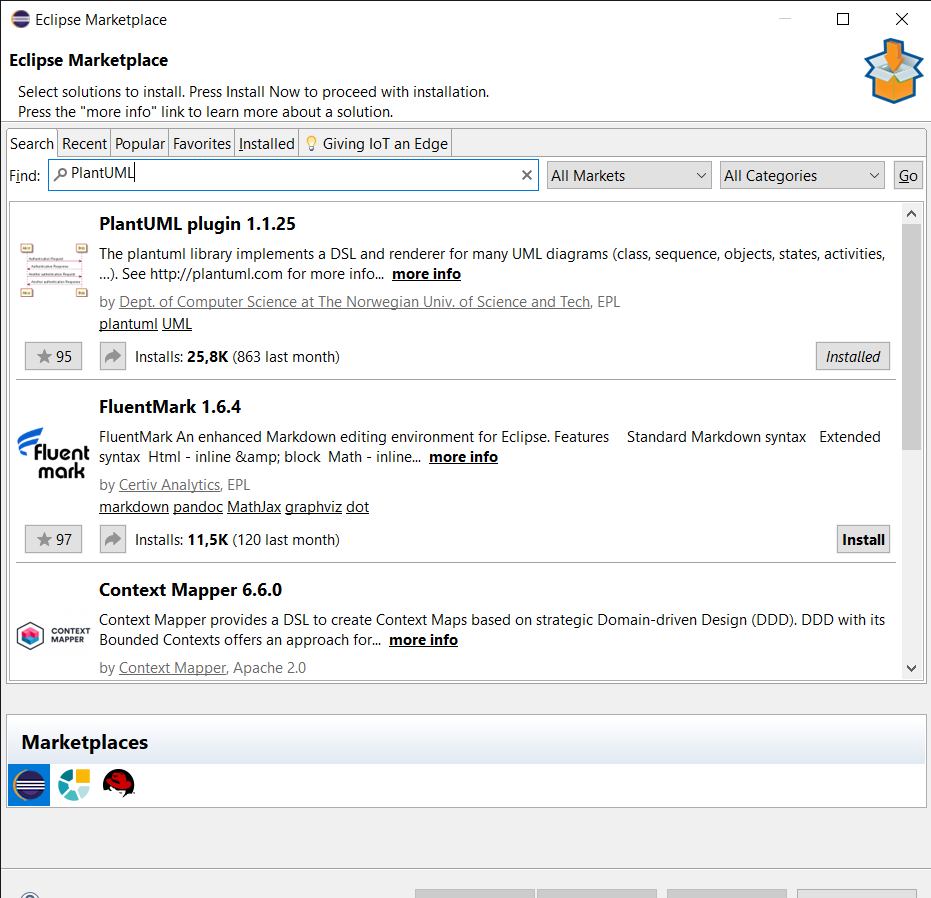
\includegraphics[scale = 0.4]{pictures/Eclipse Marketplace 08.11.2021 16_56_39.png}
    \label{screenshot marketplace}
    \caption{\centering{Screenshot of the \textit{Marketplace}}}
    
\end{figure}
\clearpage
\textbf{HiPE}: \newline\newline
Furthermor you need to install the plugin \textsf{\textit{HiPe}}. You need to click: \newline

\centering
→ \textsf{\textit{Help}} →
\textsf{\textit{Install New Software}}\newline

\raggedright
A new window should pop up and you can insert the following URL into the \textsf{\textit{Work with}} field:\newline


\centering
{\color{blue}https://hipe-devops.github.io/HiPE-Updatesite/hipe.updatesite/ \newline}

\raggedright
After pressing \textsf{\textit{Enter}} you should now see the window from the screenshot below presenting \textsf{\textit{HiPE}} next to a checkbox. Start the installation by selecting it, clicking \textsf{\textit{next}}and accepting the license agreement. In some cases you need to press \textsf{\textit{install anyway}} afterwards. Throughout the process of installing Eclipse may require a restart. If Eclipse restarts without any errors, everything necessary is installed.\newline\newline

\begin{figure}[h]
    \centering
    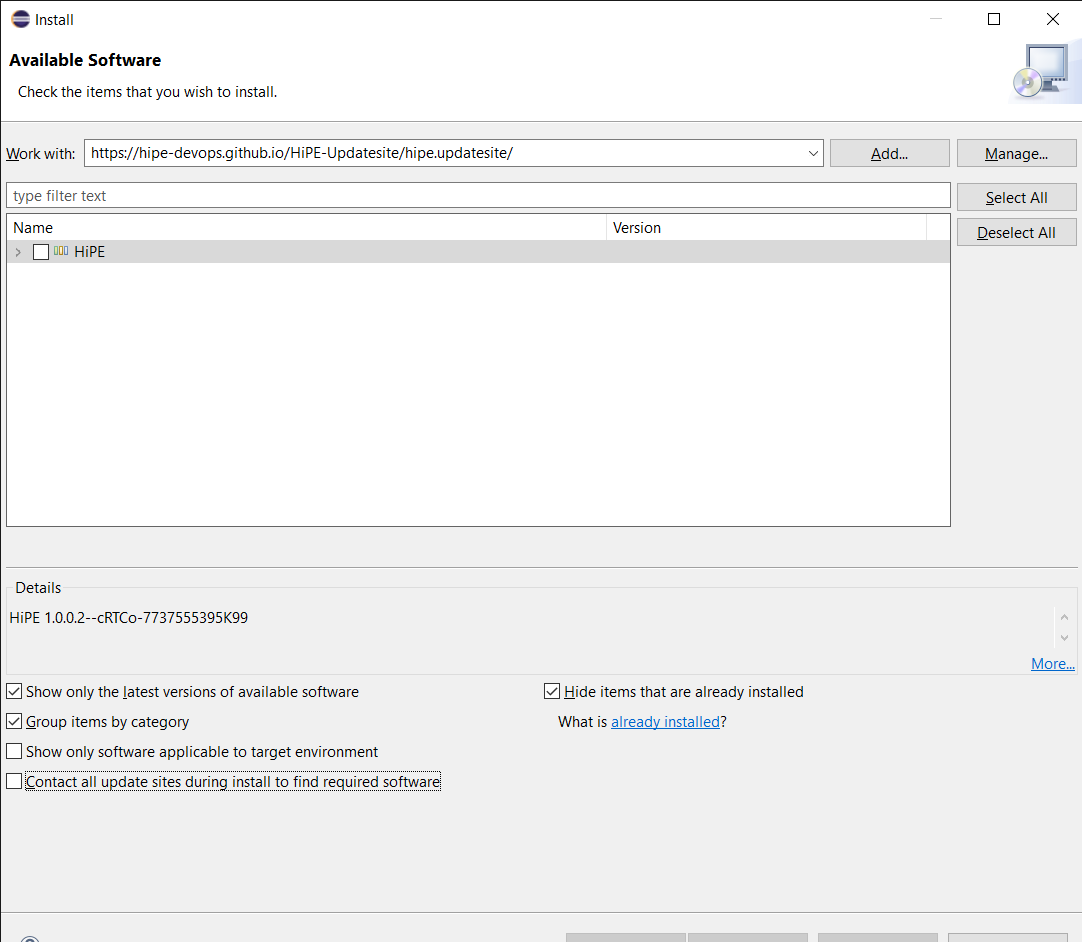
\includegraphics[scale=0.5]{pictures/eclipse_install_new_software_hipe.png}
    \caption{\centering{Screenshot of the \textit{Install New Software} window for \textsf{\textit{HiPE}}}}
    \label{screenshot install new software hipe}
\end{figure}

\clearpage

\textbf{eMoflon::IBeX:}\newline\newline
Lastly we will install \textbf{eMoflon::IBeX}. This is done in the same way as the \textsf{\textit{HiPE}} plugin. You can insert the following URL into the \textsf{\textit{Work with}} field:\newline

\centering
{\color{blue}https://emoflon.org/emoflon-ibex-updatesite/snapshot/updatesite/\newline}


\raggedright
You should now see the window from the screenshot below presenting \textsf{\textit{eMoflon:IBeX}} and it's different submodules. Although you will only need \textsf{\textit{Democles}} and \textsf{\textit{HiPE}} for this tutorial, it is advisable to install the whole suite.

Continue with the installation in the same way as in the previous step.\newline

\begin{figure}[h]
    \centering
    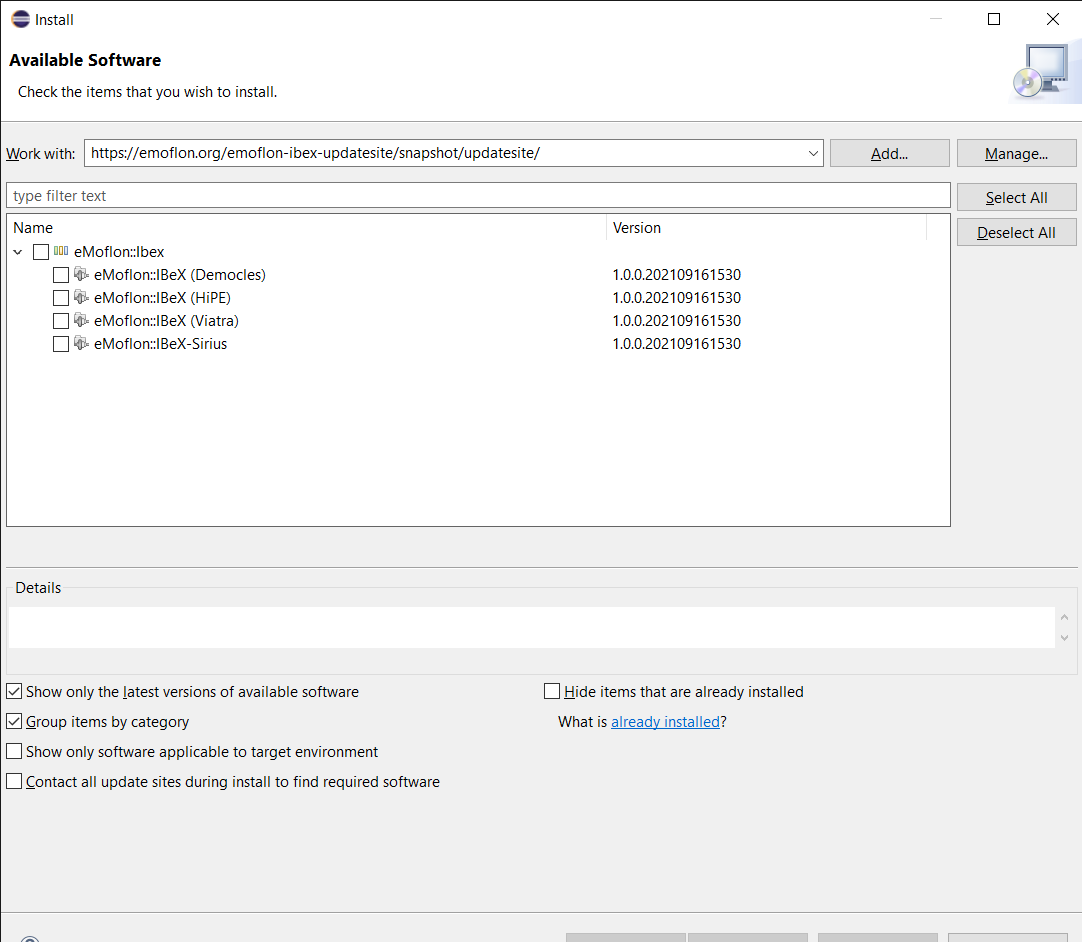
\includegraphics[scale=0.4, width =\textwidth]{pictures/eclipse-workspace - HospitalExample_model_HospitalExample.ecore - Eclipse IDE 08.11.2021 18_02_54.png}
    \caption{\centering{Screenshot of the \textit{\textsf{Install New Software}} window for \textit{\textsf{eMoflon::IBeX}}}}
    \label{screenshot install new software eMoflon::IBeX}
\end{figure}

Both \textsf{\textit{Democles}} and \textsf{\textit{HiPE}} are Eclipse projects which include pattern matching engines.

%\textsf{\textit{Viatra}} provides a framework with an editor for model queries and a code generator to implement the model queries easily into java code.
% ^Viatra is now deprecated (within eMoflon context)

\textsf{\textit{Sirius}} is a framework for visualization which implements a graphic editor for triple graph grammar rules.\newline 

In this tutorial we will just need the incremental pattern matchers of the first two. In contrast to \textsf{\textit{Democles}} \textsf{\textit{HiPE}} is a parallel pattern matcher.

\clearpage
\section{Creating a metamodel}
\subsection{Metamodeling introduction}

The first question you might be asking yourself is: What is metamodeling?

Metamodeling can be described as creating the model of a model. That means defining abstract rules and structures an instance of such a metamodel has to fulfill\footnote{See Sprinkle, Rumpe et. Al 2014 }.\newline

For a basic introduction into metamodeling and graph transformation see\footnote{\href{https://www.cs.le.ac.uk/people/rh122/papers/2006/Hec06Nutshell.pdf}{Graph Transformation in a Nutshell}}.

\subsection{Adding the eMoflon toolbar}

Now it is time to get to know the functionalities of eMoflon. Firstly you should add the \textbf{eMoflon toolbar} to your \textbf{Eclipse} as shown in the screenshot below.\newline Look for the \textit\textsf{Window} tab in the top left corner and press:\newline

\centering
→ \textit{\textsf{Window}} →
\textit{\textsf{Perspective}} → \textit{\textsf{Open Perspective}} → \textit{\textsf{Other}}
\newline

\raggedright
Then open the \textbf{eMoflon toolbar icon} which is highlighted via the red square in the screenshot below. Note that sometimes the toolbar is displayed very tiny. This can be fixed by moving the toolbar via the four dots infront of it:\newline\newline
\begin{figure}[h]
    \centering
    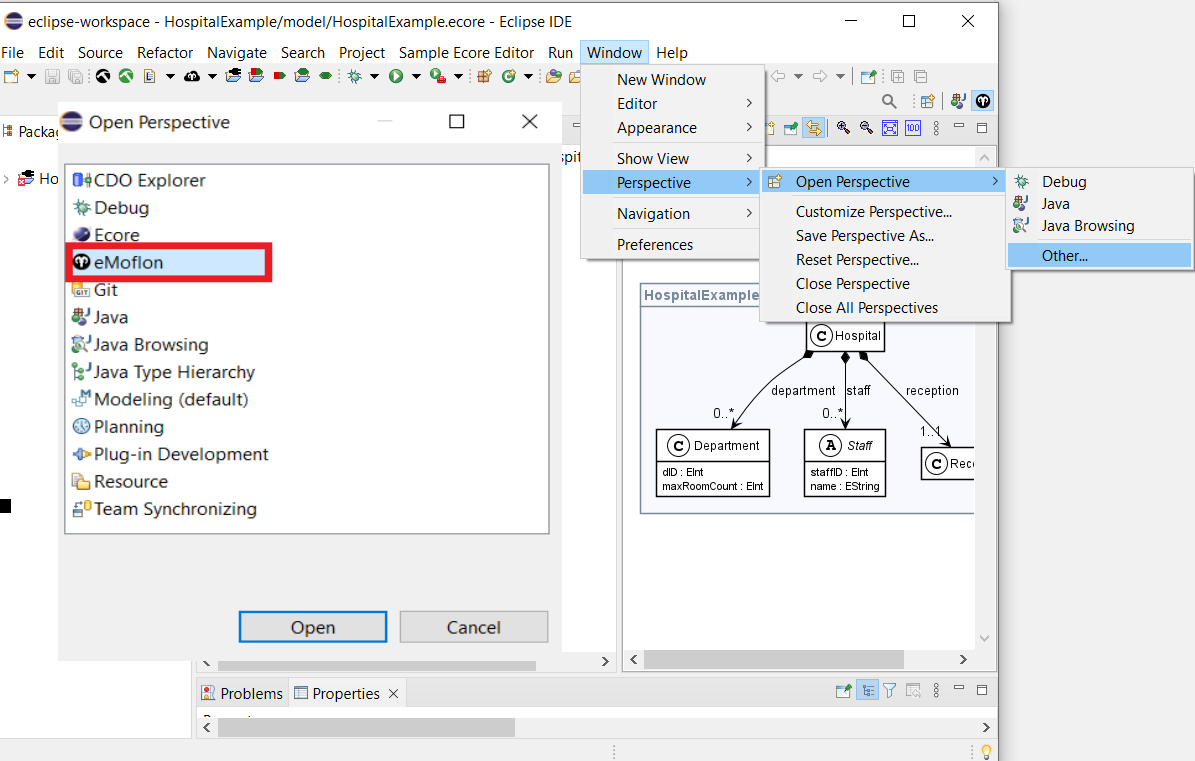
\includegraphics[scale=0.4, width =\textwidth]{pictures/add_perspective.png}
    \caption{\centering{Add the eMoflon toolbar icon}}
    \label{add toolbar}
\end{figure}

\clearpage

\textbf{Functions:\newline}

\begin{figure}[h]
    \centering
    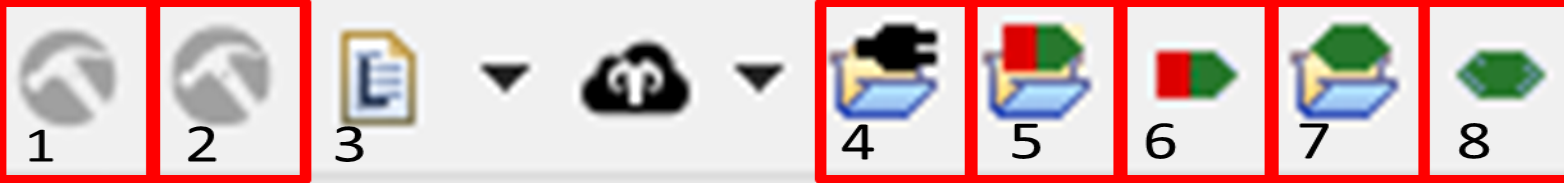
\includegraphics[scale=0.25]{pictures/toolbar_eMoflon.png}
    \caption{\centering{This is how the eMoflon perspective should look like}}
    \label{toolbar}
\end{figure}

Let us take a look at the functions we will need throughout this tutorial:

\begin{enumerate}
\item Clicking this button will \textbf{build} the selected projects \textbf{fully}.
\label{item:0}

\item Clicking this button will \textbf{build} the selected projects \textbf{incrementally}.

\item Clicking this will show you the \textbf{logging configuration} of the eMoflon Console.

\item
\label{item:1}
The folder with the plug \textbf{creates a new eMoflon project}.

\item
\label{item:2}The folder with the green and red arrow \textbf{creates a new graph transformation project}.
\item The green and red arrow \textbf{creates a simple graph transformation file}.
\item 
\label{item:3}The folder with the green trapezoid is used for \textbf{creating triple grammar graph projects}.
\item \label{tgg_rule} The green trapezoid button \textbf{creates a single triple grammar graph file}. 
\end{enumerate}

\clearpage

\subsection{Creating a new EMF project}

First of all we have to create a new \textbf{metamodel}. Click on \textbf{button 4} to create a new \textbf{\textsf{eMoflon EMF Project}} and choose a new name for your project.

For this tutorial we are going to create a scenario which models a hospital and its administration. This is supposed to show you the basic functions of eMoflon::IBeX.\newline You should \textbf{stick to the naming conventions} we are using, since inconsistent names may lead to errors later on!\newline

\centering
→ Please select \textit{\textsf{Generate default Ecore file}}\newline

\raggedright
Please give the project the name \textit{\textsf{HospitalExample}} as shown in the screenshot below. After you have pressed the \textit{\textsf{finish}} button a new file should appear in the model folder. If you cannot see it, try to refresh the folder.\newline

\begin{figure}[h]
    \centering
    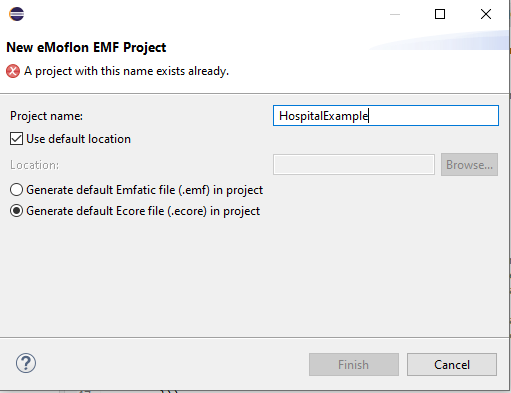
\includegraphics[scale=0.7]{pictures/project_creation.png}
    \caption{\centering{Creation of a new EMF project}}
    \label{project creation}
\end{figure}
\clearpage
\subsection{Filling the model with content}

 The chart below provides an UML-based visualization of the finished model you will create throughout this part of the tutorial. If you are not sure whether your model is correct, you can use this as a comparison:\newline
 
\begin{figure}[h]
    \centering
    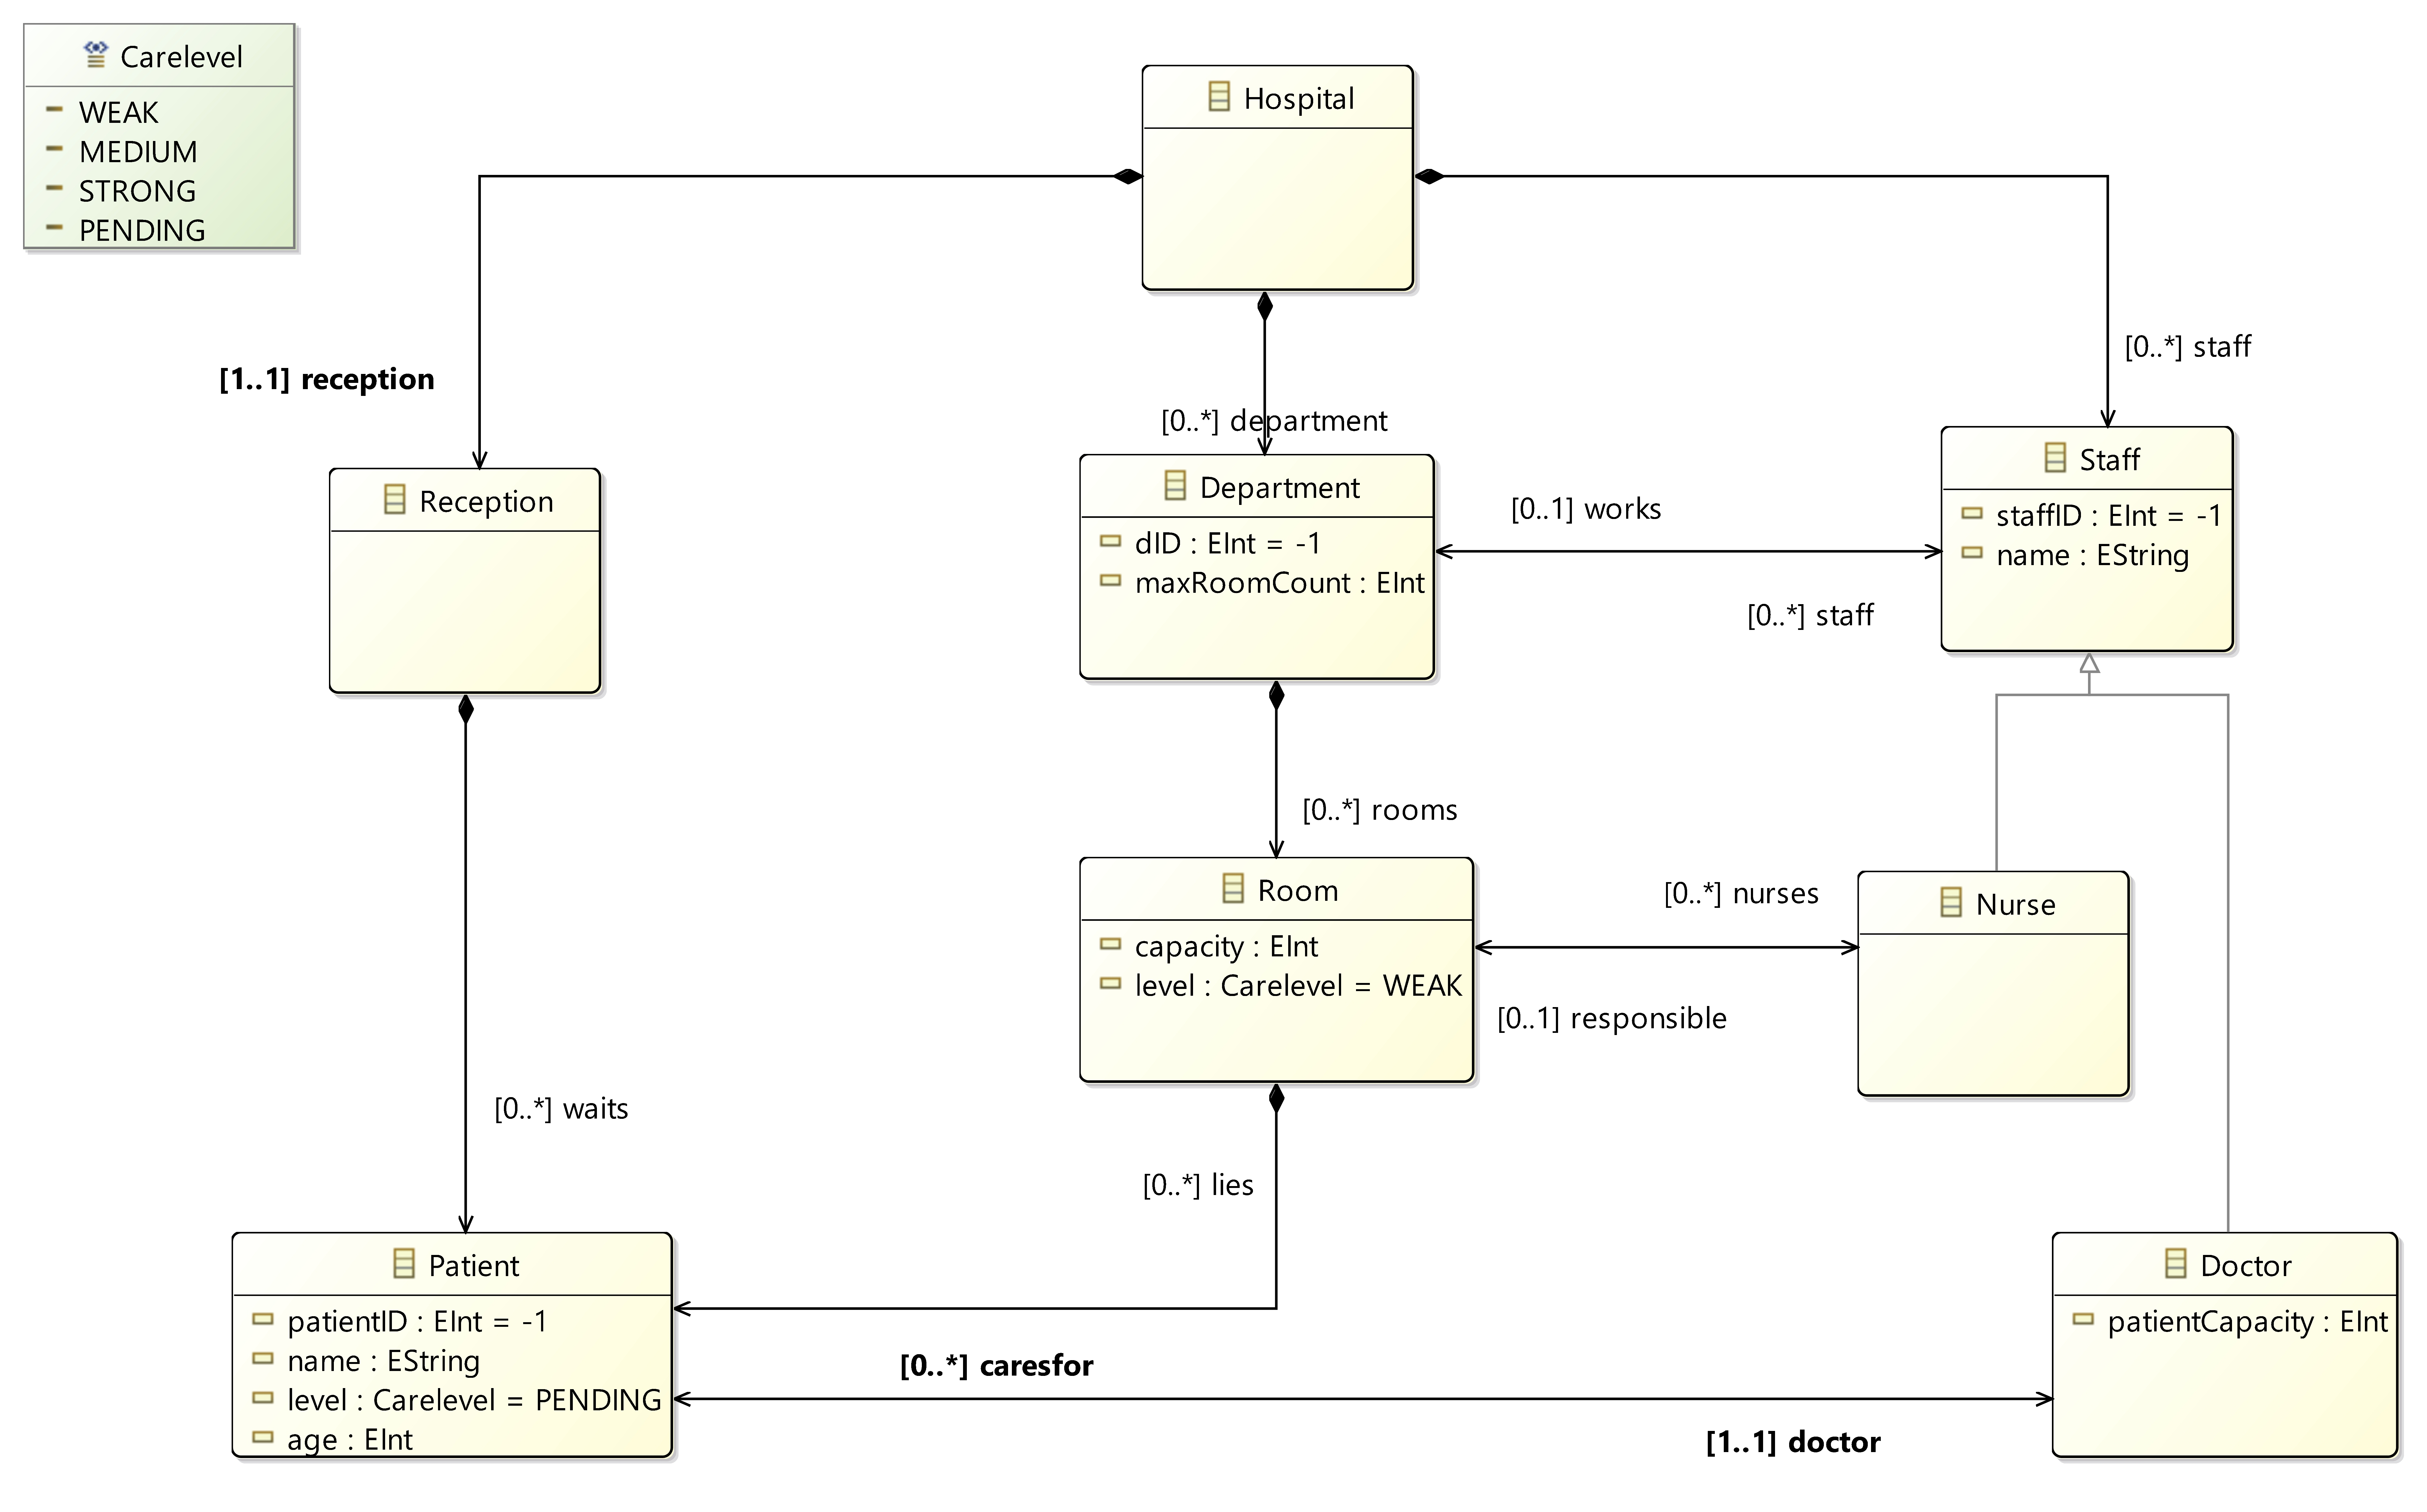
\includegraphics[scale=0.9, width= \textwidth]{pictures/model_finished.jpg}
    \caption{\centering{Complete model}}
    \label{goal model}
\end{figure}

\textbf{Note:}

To visualize your current model, left-click on \textit{\textsf{HospitalExample}} and look at the \textbf{PlantUML tab} in the top right corner. This will look a bit different than this UML chart, but should be equal in regard to its content.

\clearpage

The first class we need for our tutorial is the hospital itself. To create the \textbf{Hospital class}, you need to open the \textbf{HospitalExample.ecore package} in the model folder of your package and \textbf{right-click} it to select \textbf{EClass} as a new child of the metamodel in the drop-down menu.\newline

\begin{figure}[h]
    \centering
    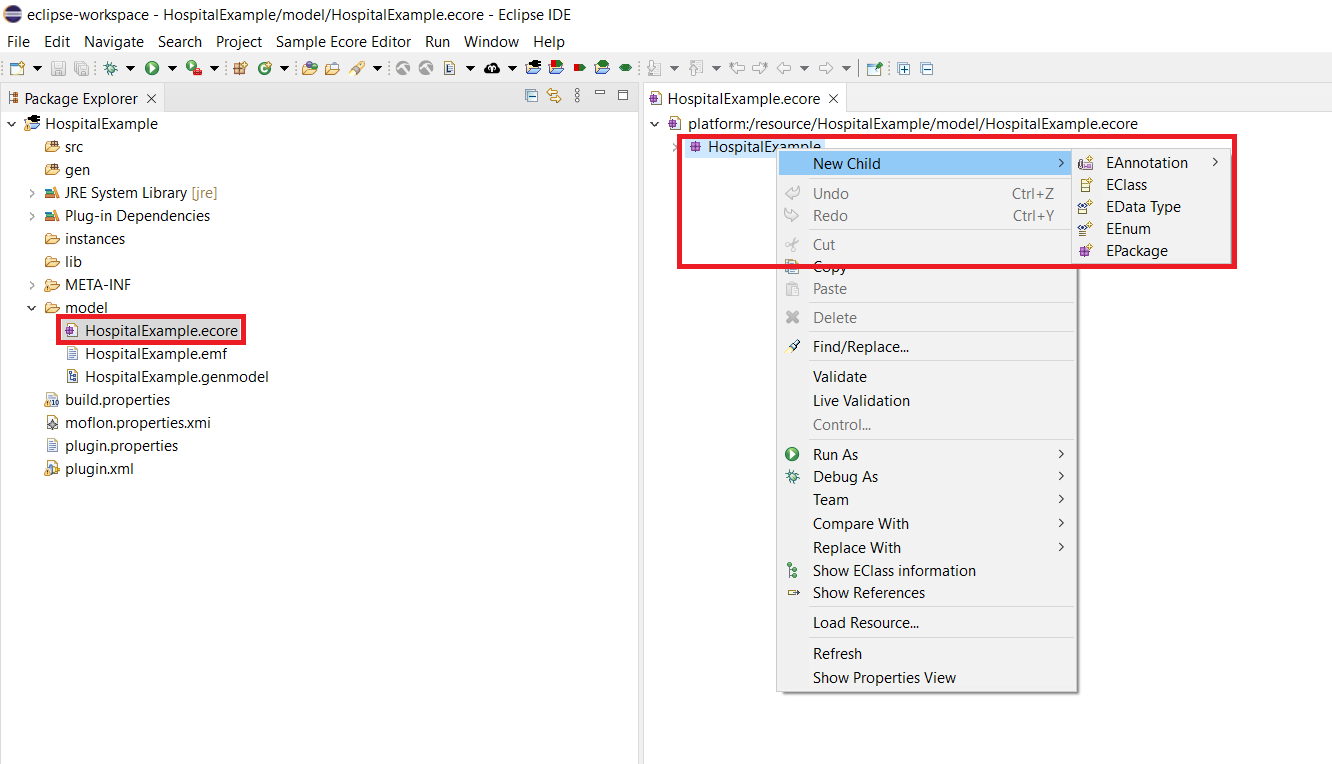
\includegraphics[scale=0.5, width= \textwidth]{pictures/new_child.png}
    \caption{\centering{Create Hospital class as child of the metamodel}}
    \label{project creation}
\end{figure}

As you can see, it is also possible to create an \textbf{enumeration}, a \textbf{data type}, and \textbf{other packages} to split up your project.\newline You may have noticed that every option begins with a capital "E". This is merely a \textbf{naming convention} used in EMF and it will be also used for things such as variable types. For example, a variable of type Integer has to be defined as "EInt".\newline

After you have created the Hospital, you can define its \textbf{properties} in the \textsf{\textit{properties}} window. If you cannot see the properties window, right-click on the \textit{\textsf{Hospital}} child you have just created and select \textit{\textsf{Show Properties View}} on the bottom of the list or \textbf{double left-click} on the child.

Let us name the class accordingly by typing \textit{\textsf{Hospital}} in the name field. All other fields can be left set to their default value.\newline

To fill our Hospital, we start by adding a \textsf{\textit{Reception}} class and a \textsf{\textit{Department}} class. This is done in the same way as for \textit{\textsf{Hospital}}.\newline

After creating the classes, we have to connect them to our hospital. This can be done by creating a \textbf{new child} of type \textbf{EReference} in our hospital class.
The properties of a \textbf{reference} offer a large variety of options you can configure but let's keep it simple for now.

To maintain comprehensibility and simplicity in your model \textbf{naming your reference} after the corresponding class or its purpose is recommended.

Hence, we chose the name \textsf{\textit{reception}}.\newline

Furthermore, we also need a \textbf{type} for our reference which can be defined in the \textbf{EType field}, where we select the type \textsf{\textit{Reception}}.\newline

Naturally, a hospital has only one reception, so we have to modify the \textbf{multiplicities} of our references as well. \textbf{Multiplicities} can be configured via the \textsf{"Lower Bound"} and \textsf{"Upper Bound"} options. By changing the \textbf{lower bound} value to \textbf{1} we ensure that our hospital has \textbf{at least one} reception. To avoid having \textbf{more than one} reception in the Hospital you have to set the value for the \textbf{upper bound} to \textbf{1} as well. If you want to model an \textbf{N-multiplicity} you have to set the \textbf{upper bound} to \textbf{-1}.\newline

Please note that it is also possible to change the \textbf{boundaries of attributes}. However, meddling with the attribute boundaries can easily mess up your model. Hence, we advise you to leave the boundaries of attributes as they are by default.\newline

The model depicts the relation between the Hospital and the Department class with a \textbf{rhomb} this means the relationship is a \textbf{containment}. You have to set the value of the \textsf{"Containment"} field to \textsf{true}.\newline

Please create the \textbf{department reference} analogously. This time the reference has an N-multiplicity, which can be modeled like shown above. Note that you can get the correct multiplicities and the correct type of an attribute by looking at Figure 7.\newline

A short note on \textbf{containment objects}: If you delete a container object, e.g., the Hospital in our case, you will also delete every object that is contained by the Hospital. In addition, an object can only be contained by one container, once a new containment edge is assigned to an object the old containment edge will be deleted.\newline

For the next step, we want to assign attributes such as department numbers and a maximum number of rooms for our departments, to our Department class. Add a \textbf{new child} of the type \textbf{EAttribute} to the departments, name it \textsf{"dID"}, and give it the type \textsf{"EInt"} in the EType field. Since we want every department to have an ID, we modify the \textbf{multiplicities} in the same manner as our previous references.
Also set the field \textsf{"ID"} to \textsf{true}. This tells the model whether the value of this attribute identifies the object uniquely in the containing resource.
\newline
Create the Attribute \textsf{"maxRoomCount"} analogously except it won't be used as an \textbf{ID}.\newline

Before we continue we want to create something in our model that symbolizes the different care levels in a hospital. Suitable for this is an \textbf{enumeration}. The \textsf{Carelevel} enumeration can be created as a child of the Hospital package. The possible care levels should be \textsf{WEAK}, \textsf{MEDIUM}, \textsf{STRONG} and \textsf{PENDING} which can be added as \textbf{children of the enumeration} of type \textbf{EEnum literals}.\newline

Naturally we need patients in our hospital as well. \textbf{Patients} have the following attributes: A  \textsf{name}, a \textsf{patientID,} and a \textsf{level} representing the \textbf{care level} assigned to a patient.
Please create the \textbf{Patient class} accordingly.\newline

When a patient arrives at the hospital he will be waiting in the reception until he has been assigned to a room and diagnosed with necessary treatment. For the first condition, we need a \textbf{reference in the reception class} to the patient and while the patient is waiting in the reception he has not been diagnosed yet. Hence, we want to set the \textbf{default value literal} of the \textbf{level attribute} to \textsf{PENDING}.\newline

The attribute \textsf{maxRoomCount} already indicates the need for a \textbf{room class}. Regarding the \textbf{attributes} of the rooms, we need a \textbf{capacity} and a \textbf{care level} to indicate the necessary medication for the patients and the room.
For the latter you can select our freshly created enumeration \textsf{Carelevel} as its \textbf{attribute type}. The \textbf{default value} for the level should be \textsf{WEAK}.
Please create the room class accordingly.\newline

The rooms also need a \textbf{connection to the departments} they are assigned to and \textbf{contain} multiple patients. Please add \textbf{references} in the \textbf{Department class} to model this. You can get their characteristics from the final model in fig \ref{goal model}.\newline
% and the responsible staff.

After creating the infrastructure for our hospital, we need the people, which are required to keep a hospital running and of course the patients. Starting with the Staff, create an \textbf{abstract class} with the \textbf{attributes} \textsf{staffID} of the type "EInt" and the \textsf{name} of the staff member which should be an "EString". You can set the class to abstract by selecting \textsf{true} for the field \textsf{Abstract} in the properties window.\newline
Similar to the concept of inheritance in Java it is not possible to instantiate such a class. However, attributes and variables defined in an abstract class will be inherited by a subclass of this abstract class.\newline

The staff should be \textbf{contained in the hospital} and needs a \textbf{reference} to the department the staff member is working in.
The staff needs to be differentiated into nurses and doctors. Create a new \textbf{Doctor class} and change the \textsf{ESupertype} in the properties window to \textsf{Staff}, which allows the Doctor class to \textbf{inherit the references and attributes} of the \textbf{abstract Staff class}. This can be done by pressing \textsf{Add} and confirming in the windows that will pop up.
Additionally, we want to add the \textbf{attribute} \textsf{patientCapacity} to define the number of patients a doctor can care for and a relationship to the patients he oversees.\newline
For the Nurse class, we want a reference to the rooms a nurse is \textsf{responsible} for. 

To model this responsibility we want a \textbf{bidirectional reference} between the \textbf{Doctor class} and the \textbf{Patient class}.
To achieve bidirectional references please create a \textbf{reference} in the \textbf{patient class} to the doctor called \textsf{doctor}. On the other hand create a \textbf{reference} to the patient class in the \textbf{doctor class} called \textsf{caresFor}. Multiplicities can be read from fig \ref{goal model}.
Now for the latter select the reference \textsf{caresfor:Patient} in the \textbf{EOpposite property}. This should be done automatically but if not, go to the \textbf{doctor class} and assign the \textsf{doctor:Doctor} reference as an \textbf{EOpposite} of the created reference as well.\newline
\textbf{Note}: This works only if you have set the type correctly and if the opposite reference has been created already.\newline

Please follow the same procedure to make the existing \textbf{reference between the nurse class and the room class bidirectional}.\newline

Also add a \textbf{bidirectional reference} between the \textbf{staff} and the \textbf{department} they are \textsf{working} in.\newline

If you made it this far your hospital meta-model should be completed and the visualization in PlantUML should look like this:

\begin{figure}[h]
    \centering
    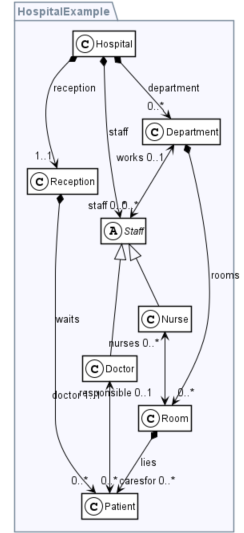
\includegraphics[scale=0.7]{pictures/goal_vis_PlantUML.png}
    \caption{\centering{Goal model in PlantUML}}
    \label{plantUml goal}
\end{figure}

Please also compare your \textbf{Multiplicities}, \textbf{attributes}, \textbf{default literal values}, \textbf{containment values} and all \textbf{names} to fig \ref{goal model}. Differences can result in errors later on.\newline

Congratulations on completing the first part of this tutorial!

\clearpage

\section{Graph transformation with eMoflon}

The next part of our Tutorial is dedicated to the creation of a graph transformation rule set which allows us to create a concrete model instance based on constraints and multiplicities we defined in this metamodel. The goal of the ruleset we want to define in the next chapter is to achieve the defined structure and behavior of operations in our hospital while creating a certain kind of dynamic through the application of rules. This might sound a bit confusing for now, but no worries we will explain it to you step by step.

\subsection{Rules and patterns introduction}

%The GitHub site where you have found this PDF for the Tutorial also has different stages of the project stored for you in case you messed something up, skipped a part of the tutorial, or if you are unsure whether everything you did is correct.
%These different stages of the project are represented by different branches in the Git repository. Throughout this tutorial, we will be using four different branches which you can access to keep the project up to date for every section of the tutorial. Whenever you can switch to a new branch for a new section it will be announced at the beginning of the respective section.\newline

%\textbf{Please use the branch \textsf{Ecore+GT empty} for the following section}.
%This stage of the project includes the hospital ecore model and the graph transformation project you just created in the previous chapter but has some repetitive contents added to it so that you can focus on the important functionalities.\newline
%Whenever you have to add code to the existing project it will be said \textbf{explicitly} and \textbf{highlighted in the Java project}.\newline*/

Now that you are good to go, it is time to get familiar with the two most common constructs for eMoflon Graph Transformations: \textbf{The rules and patterns}. For a more detailed description you can read the second chapter of this essay\footnote{\href{https://www.cs.le.ac.uk/people/rh122/papers/2006/Hec06Nutshell.pdf}{Graph Transformation in a Nutshell}}.\newline

\textbf{Graph pattern}:\newline
A Graph pattern describes certain structures that must be present in a given instance graph. A structure consists of an arangement of nodes with specific types and specific connecting edges. A pattern could also be made up by a single node of a specified type.\newline
\begin{figure}[h]
    \centering
    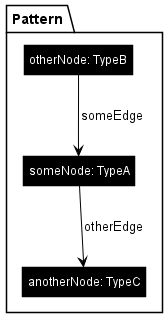
\includegraphics[scale=0.7]{pictures/pattern.png}
    \caption{\centering{Pattern example in PlantUML}}
    \label{pattern example}
\end{figure}

Consequently, a graph pattern matcher will find all sub-structures in the instance graph that match all structural constraints of a given pattern.\newline
\clearpage

\textbf{Graph transformation rule}:\newline\newline
A graph transformation rule consists of a so-called left-hand side (LHS) and right-hand side (RHS). The former describes certain preconditions, like a graph pattern that must be present in a given instance graph, otherwise a rule is not applicable. If a match of the LHS is found, the rule can be applied. When a rule is applied, the graph is changed in such a way, that the rule's RHS is satisfied. More precisely, any graph pattern node and edge that is present in the LHS, but is not present in the RHS, is deleted. In turn, any node that is not present in the LHS, but is present in the RHS, is created.\newline

\begin{figure}[h]
    \centering
    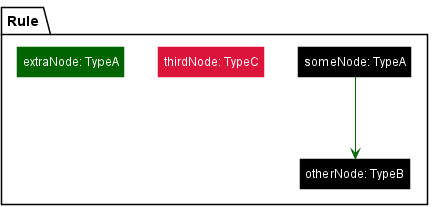
\includegraphics[scale=0.8]{pictures/rule.png}
    \caption{\centering{A rule example in PlantUML}}
    \label{rule}
\end{figure}

\clearpage

\subsection{Creating a graph transformation project}

Let us get started by creating a new eMoflon Graph Transformation project. Please click on the button \ref{item:2} with the \textbf{red and green arrow in the folder}.\newline\newline

\centering

→ Please write \textsf{"HospitalTransformRules"} as the name → Press \textsf{"Finish"} \newline\newline

\raggedright

You will notice the \textsf{Rules.gt} file which has been generated automatically. In this file, you will be defining the rules to construct our Hospital.\newline
Start with deleting the automatically generated contents in the “.gt” file except for the Ecore import.

The next thing you want to do is to \textbf{import the metamodel} you have created in the previous section. Just type import and use code completion (Ctrl+Space) to obtain the suggested URI to your metamodel HospitalExample.\newline

Afterwards your \textsf{Rules.gt} file should be empty exept these two imports:\newline

{\setstretch{1.2}

1\hspace{0.5cm}\textcolor{Purple}{import} "\textcolor{Blue}{http://www.eclipse.org/emf/2002/Ecore}"

2\hspace{0.5cm}\textcolor{Purple}{import} "\textcolor{Blue}{platform:/resource/HospitalExample/model/HospitalExample.ecore}"\newline

}

You might have noticed that the project has some \textbf{compilation errors}. To solve the issues do the following:\newline\newline

\centering

Open \textsf{"META-INF/MANIFEST.MF"} file → \textsf{dependencies} → Add \textsf{"HospitalExample"} to the Required Plug-ins menu.\newline\newline

\begin{figure}[h]
    \centering
    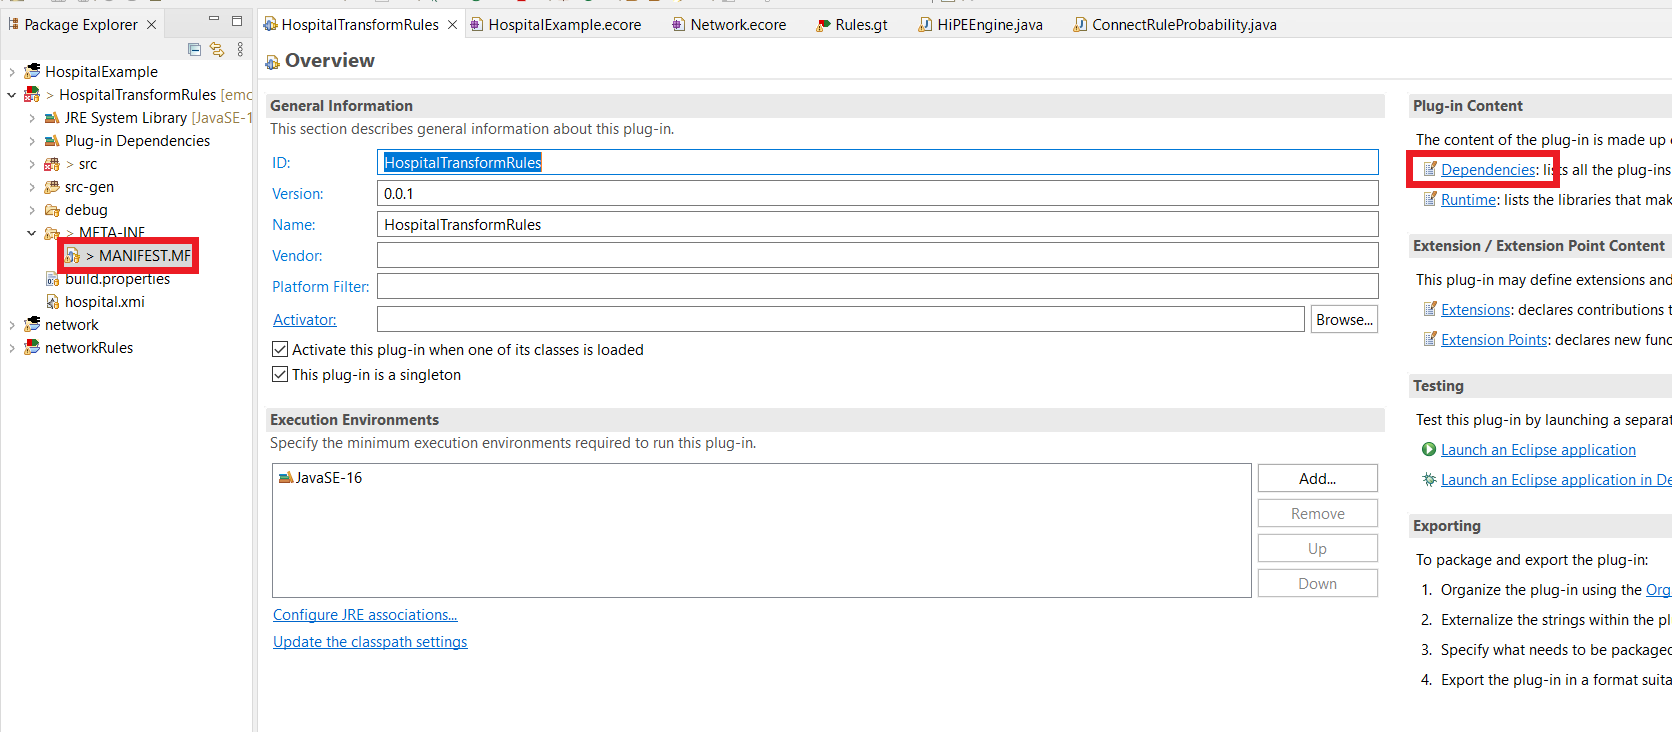
\includegraphics[scale=0.7, width= \textwidth]{pictures/manifest.png}
    \caption{\centering{Manifest.MF}}
    \label{manifest}
\end{figure}

\raggedright

The errors should be fixed now, and your project should compile properly. If the \textbf{errors persist} check if the Build automatically option is turned on in the project drop-down menu of your eclipse. \textbf{Refreshing and cleaning} all the projects are the remaining options if you are still encountering errors. Should there still be errors remaining in the manifest, check the code of the manifest for the \textbf{Export-Package} and \textbf{Import-Package} sections and check if the names are written properly. Sometimes the commas and names get mixed up or put in the wrong line. After fixing that you should see no more errors.

\raggedright

\clearpage
\subsection{Rules and patterns in eMoflon}

Anyhow, let us get started by writing the very first rule for our hospital rule set. The complete hospital ruleset will allow us to create a concrete hospital model instance according to the specifications of our metamodel from chapter one. Graph transformation rules are perfectly suited for this task since they allow us to consider constraints and requirements directly.\newline

\textbf{Rules:}\newline
For a rule, we need the \textbf{keyword rule} and a \textbf{name for the rule}. As previously mentioned, you should \textbf{name the rule after its purpose} to keep the project comprehensive.\newline

As a brief introduction to our syntax, we would like to present the two most important operators:

\begin{itemize}
    \item \textcolor{LimeGreen}{[+]} 
    \item {\color{red} [--] }
    \item {[=]}
\end{itemize}
Any Element that is prepended with a \textcolor{LimeGreen}{ [+]} is \textbf{created} when the rule is applied. This is indicated by the \textcolor{LimeGreen}{ green syntax color}.\newline

In turn, the {\color{red} [--] } operator will lead to a \textbf{deletion} of the denoted element. If an element is deleted by the application of a rule the {\color{red}syntax will be colored red}. \newline

If the {[=]} operators is used, the element is interpreted as \textbf{context} and \textbf{colored black}.\newline

Every element that is \textbf{not denoted} with an operator describes the \textbf{LHS} of the rule, which means that these elements must be present in a given instance graph.\newline
In practical terms, a valid match of the LHS must be present before the rule can be applied.\newline
By using the \textcolor{LimeGreen}{[+]} operator before the hospital graph pattern node in the hospital rule, we enable the rule to create a new hospital Object upon application. Since this rule has no black or red context elements, it can \textbf{always} be applied. \newline

{\setstretch{1.2}

1  \hspace{0.5cm}  \textcolor{Purple}{rule} hospital() \{\newline
2  \hspace{1cm}  \textcolor{LimeGreen}{[+] hospital: Hospital}\newline
3  \hspace{0.5cm}  \};\newline

}

\textbf{Patterns:}

If we want to check whether a hospital object is present within a given model, we can create a pattern that finds a hospital. Here we create the pattern \textsf{findHospital()} that defines a node named hospital of the type Hospital. Since no elements are annotated with any of the operators, findHospital() only contains black elements, i.e., context and will not lead to the creation or deletion of any objects.\newline
Therefore, findHospital() is not a rule, but a pattern, which solely will instruct the pattern matching engine to \textbf{find matches of this pattern}.\newline

{\setstretch{1.2}

4 \hspace{0.5cm}	{\color{Purple}pattern} findHospital() \{\newline
5 \hspace{1cm}	{[=]} hospital: Hospital\newline
6 \hspace{0.5cm}	\};\newline

}

\textbf{Please create rule and pattern in the \textsf{Construction.gtl} file of your \textsf{HospitalTransformRules} project.}\newline

\textbf{Note on patterns}:
\newline
Just like shown in this example, all the other patterns for all the other types should be created by you on your own.\newline

\textbf{Note on the visualization of PlantUML}:
\newline
When you click on the freshly created hospital rule you should see the visualization in the PlantUML window on the right. It shows you the rule and the way the rule is defined as a graph structure. The black boxes are pattern nodes that represent context, as a consequence these nodes must be present in an instance graph. Analogously, black arrows define context edges between nodes, that must be present in the same instance graph. The green elements are the ones we are creating with a rule application.

\clearpage

\subsection{Application Condition}

Since our model requires only one hospital node, we should add a so-called \textbf{application condition} to prevent multiple applications of the hospital rule.\newline

Please note there are two types of conditions. You can either \textcolor{Purple}{forbid} the presence of graph structures attached to pattern matches or \textcolor{Purple}{enforce} them.
An application condition that forbids the presence of such structures is called a \textbf{negative application condition (NAC)} while a condition that enforces the presence of such structures is called a \textbf{positive application condition (PAC)}.
\newline
The utilization of a construct consisting of a condition and a pattern is called a \textbf{support pattern invocation} while the pattern itself is called a \textbf{support pattern}.\newline \newline
Back to the example. To extend our hospital rule with a negative application condition, add a \textcolor{Purple}{forbid} inside our hospital rule and insert \textsf{findHospital} into the round brackets as the name of pattern to be forbidden.\newline
With our condition, we want to forbid the application of the rule if our \textsf{findHopistal} pattern finds the structure \textsf{hospital:Hospital}.\newline

{\setstretch{1.2}

1 \hspace{0.5cm} \textcolor{Purple}{rule} hospital() \{ 

2 \hspace{1cm} \textcolor{LimeGreen}{[+] hospital: Hospital}

3 \hspace{1cm} \textcolor{Purple}{forbid}(findHospital) [] 

4 \hspace{0.5cm} \};\newline

}

After creating a rule for the construction of a hospital node we need to fill our hospital with the same objects of our meta-model. So, let us continue with a \textbf{reception}. We start by creating the rule \textsf{reception} and adding a reception node of type reception.\newline

In contrast to the previous rule, we also have to \textbf{link our reception to the hospital}. To create such a reference, we require the hospital node and add an edge from the hospital node to the reception node as we have done previously in the tutorial.\newline You need to use the \textcolor{LimeGreen}{[+]} operator once again but now we continue with a \textbf{"-"}. This marks the created structure as an edge. The \textbf{“-"} is followed by the \textbf{type of the edge} and with \textbf{“->”} we are pointing towards the \textbf{node we want to connect}.\newline
The syntax should look like depicted below and the crucial part for the creation of an edge is shown in \textbf{line 9}:\newline
Additionally we now need to add some code into the brackets after the forbid() statement. There we need to specify which node of a pattern \textbf{maps} to a corresponding node of a second pattern. We do this by adding \textbf{hospital=hospital} into the brackets.\newline

{\setstretch{1.2}

5 \hspace{0.5cm}\textcolor{Purple}{rule} reception() \{

6 \hspace{1cm}    [=] hospital: Hospital \{

7 \hspace{1.5cm}       \textcolor{LimeGreen}{[+] -reception -> reception}

8 \hspace{1.5cm}	 \}

9 \hspace{1cm}	 \textcolor{LimeGreen}{[+] reception: Reception}

10 \hspace{1cm}\textcolor{Purple}{forbid}(findReception) [hospital=hospital] 

11 \hspace{0.5cm}\}; \newline

}

\textbf{Please implement both rules above this chapter in your rules file.}\newline

An example for an application of enforce would be:

{\setstretch{1.2}
	
	1 \hspace{0.5cm}\textcolor{Purple}{rule} releasePatient(patientID:EInt) \{
	
	2 \hspace{1cm}    ...
	
	3 \hspace{1cm}	\textcolor{Purple}{enforce}(findPatientInRoom)[patient=patient]
	
	7 \hspace{0.5cm}\}; \newline
	
}

\clearpage

\subsection{Parameters and attribute constraints}

The focus of this chapter will be the handling of parameters in rules and attribute constraints.
Regarding the infrastructure of our hospital, we have to address the \textbf{departments} and \textbf{rooms} in our next rules.\newline

You should be able to create the \textbf{department rule and the branch} from the hospital node yourself. We will expand them now.\newline

After creating these two rules we want to introduce some new syntax. Remember that both classes have attributes that need to be assigned. To assign \textbf{attributes} you need to use the \textbf{operator “.”}. Pressing the \textbf{auto-completion} behind the "." should suggest the \textbf{attributes defined in the meta-model}.\newline By typing the \textbf{operator “:=”} you can \textbf{assign a value} to the attribute, e.g. the simplest assignment would be a static one.\newline
As an \textbf{unrelated} example for this, you could assign the \textsf{ID 1} to the department you create by writing: \newline

1 \hspace{0.5cm} .\textcolor{LimeGreen}{dID}:=\textcolor{Purple}{1}. \newline

In reality we want to hand over a \textbf{parameter}, not unlike it is done in Java methods.\newline
We need to define the parameters the rule expects in the \textbf{round brackets} after the rule name and type \textbf{parameter.}\textsf{paramName}; instead of the static assignment. The same has to be done for \textsf{maxRoomCount}:\newline\newline

{\setstretch{1.2}

1\hspace{0.5cm} \textcolor{Purple}{rule} department(dID: EInt, maxRoomCount: EInt)\{\newline
2\hspace{1cm}	[=] hospital: Hospital \{\newline
3\hspace{1.5cm}	\textcolor{LimeGreen}{[+] -department -> department} \newline
4\hspace{1cm}	\}\newline
5\hspace{1cm}   \textcolor{LimeGreen}{[+] department: Department} \{ \newline
6\hspace{1.5cm}	    .\textcolor{LimeGreen}{dID}:=\textcolor{Purple}{parameter}.dID; \newline
7\hspace{1.5cm}	    .\textcolor{LimeGreen}{maxRoomCount}:=\textcolor{Purple}{parameter}.maxRoomCount; \newline
8\hspace{1cm}		\} \newline
9\hspace{0.5cm}\}; \newline\newline

10\hspace{0.5cm} \textcolor{Purple}{rule} room(cap: EInt, carelvl: Carelevel) \{ \newline
11\hspace{1cm}		[=] hospital: Hospital \{ \newline
12\hspace{1.5cm}			[=] -department -> department \newline
13\hspace{1cm}		\} \newline
14\hspace{1cm}		[=] department: Department \{ \newline
15\hspace{1.5cm}\textcolor{LimeGreen}{[+] -rooms -> room} \newline
16\hspace{1cm}	\} \newline
17\hspace{1cm}	\textcolor{LimeGreen}{[+] room: Room} \{ \newline 
18\hspace{1.5cm}	.\textcolor{LimeGreen}{capacity}:= \textcolor{Purple}{parameter}.cap; \newline
19\hspace{1.5cm}	.\textcolor{LimeGreen}{level}:= \textcolor{Purple}{parameter}.carelvl; \newline
21\hspace{1cm}\} \newline
22\hspace{1cm}	\textcolor{Purple}{[\#]}department.maxRoomCount>\textcolor{Purple}{count}(findRoomInDepartment)[department=department]; \newline
23\hspace{0.5cm}\}; \newline\newline

}

\textbf{Please implement both rules above this chapter in your rules file.}\newline

\clearpage

\textbf{Attribute constraints:}

For the room rule, we want to add a \textbf{constraint} that limits the creation of rooms in a certain department because we have previously limited the maximum number of rooms a department can contain. To specify a so-called \textbf{attribute constraint (or attribute condition)} you have to use the \textbf{“[\#]”} operator. Such an attribute constraint can be defined at any point in the pattern. For this constraint, we want to get the \textsf{maxRoomCount} of the given Department and check if the limit of rooms in this department is not exceeded.

To \textbf{access an attribute value} of a specific pattern node, we provide a syntax that is remarkably similar to accessing attributes in java, namely using the \textbf{"."} operator.\newline
For example, we access the parameter of the department node via \textsf{[\#]department.maxRoomCount}. The \textsf{ count(findRoomInDepartment)} instruction \textbf{counts the matches} for a certain pattern, in our case for the \textsf{findRoomInDepartment} pattern which we have to create in the next step.\newline

\textbf{Support pattern invocations with mapping:}\newline
Our goal for this pattern is to count the number of rooms which are assigned to a department. However, we want to avoid finding matching rooms connected to any department node since this would lead to \textsf{n·m} matches for \textsf{n} rooms and \textsf{m} departments.\newline Consequently, we want to count the matches for the rooms assigned to a \textbf{single} department node. In other words we want the \textbf{graph pattern matcher} to only find matches of our \textbf{pattern} \textsf{findRoomInDepartment()} that involve the \textbf{specific department node} we are currently referencing in our \textbf{rule} \textsf{room}. To accomplish this we have to create a \textbf{mapping} between the nodes in the rule and the elements in the support pattern. eMoflon will do exactly that if we \textbf{assign identical names} for the nodes in rules and patterns.\newline

Generally, patterns which are used like this, are invocated from the \textbf{'perspective'} of the currently evaluated element. eMoflon will try to resolve identifiers from the pattern as \textbf{references} to structures from the surrounding element. If matching names are found the corresponding element will be regarded as a placeholder for any node, reference or else of matching type. These kinds of pattern invocations are also called \textbf{support pattern invocations} just like \textbf{NACs} and \textbf{PACs}.\newline

You can note the difference when comparing these slightly different patterns:\newline

{\setstretch{1.2}

1\hspace{1cm}\textcolor{Purple}{pattern} findRoomsInAnyDepartment()\{  

2\hspace{1.5cm} [=] otherdepartment:Department \{  

3\hspace{2cm} [=] -rooms->otherroom 

4\hspace{1.5cm} \} 

5\hspace{1.5cm} [=] otherroom: Room 

6\hspace{1cm}\};\newline 

}

When called as a support pattern \textbf{in context of the rule} \textsf{room} this will find $n \times m$ matches since it doesn't reference any structure from our rule and consequently would be valid for any rooms in any department node.\newline

\begin{figure}[h]
    \centering
    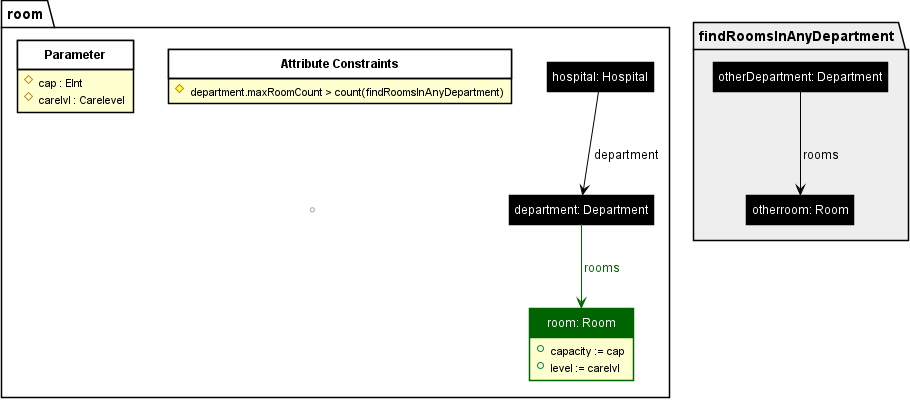
\includegraphics[scale=0.45]{pictures/findRoomsInAnyDepartment.png}
    \caption{\centering{PlantUML visualization of findRoomsInAnyDepartment}}
    \label{findRoomsAny}
\end{figure}

\clearpage


{\setstretch{1.2}

7\hspace{1cm}\textcolor{Purple}{pattern} findRoomsInDepartment()\{  

8\hspace{1.5cm} [=] department:Department \{

9\hspace{2cm} [=] -rooms->otherroom 

10\hspace{1.5cm} \} 

11\hspace{1.5cm} [=] otherroom: Room 

12\hspace{1cm}\};\newline 

}

When called as a support pattern \textbf{in context of the rule} \textsf{room} this will find this pattern will find all rooms for the \textbf{specific} department node referenced in our rule.

\begin{figure}[h]
    \centering
    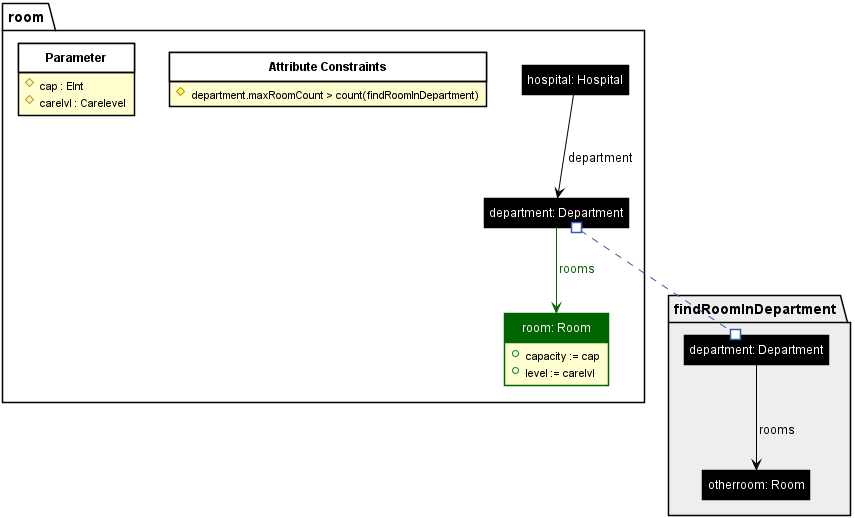
\includegraphics[scale = 0.45]{pictures/roomRule.png}
    \caption{\centering{PlantUML visualization of findRoomsInDepartment}}
    \label{findRooms}
\end{figure}

{\setstretch{1.2}

13\hspace{1cm}\textcolor{Purple}{pattern} findRoomInDepartment()\{  

14\hspace{1.5cm} [=] department:Department \{ 

15\hspace{2cm} [=] -rooms->room 

16\hspace{1.5cm} \} 

17\hspace{1.5cm} [=] room: Room

18\hspace{1cm}\};\newline

}

When called like the others this pattern will find exactly find 1 match. Because we are not only referencing the department node from our rule but the specific room we have just created as well.

\begin{figure}[h]
    \centering
    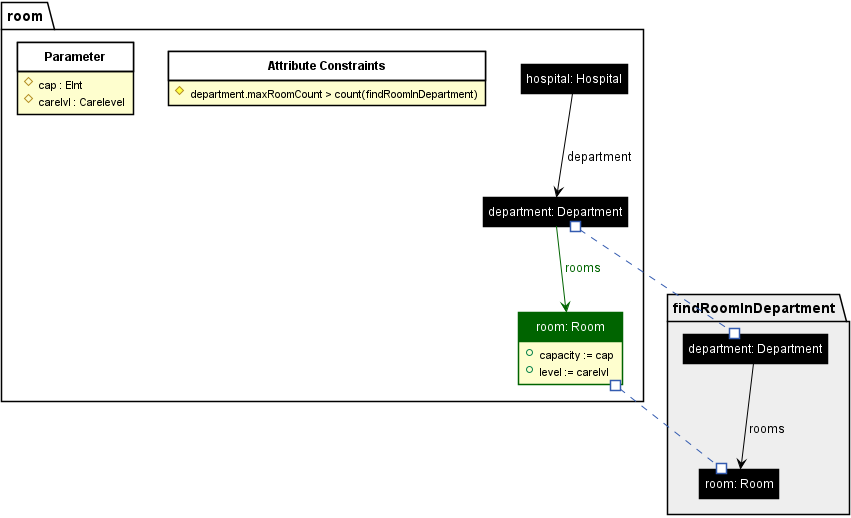
\includegraphics[scale = 0.43]{pictures/findRoomInDepartment.png}
    \caption{\centering{PlantUML visualization of findRoomInDepartment}}
    \label{attributeConstrains}

\end{figure}

Note that you can look at the PlantUML visualization of rules and pattern by clicking on them in the \textsf{Construction.gtl} and looking at the PlantUML view. \newline

Please use the \textsf{findRoomInDepartment} pattern for our room rule.\newline

\textbf{Disclamer control flow:}\newline
While attribute constraints and conditions can be used to model complex application conditions for rules and patterns
it's not possible to model \textbf{control flow} directly in eMoflon. For example you can not specify on which of all fitting elements a rule will be applied or in what order new elements will be created.

This has to be done in the actual code implementation.



\clearpage

\subsection{Finishing the graph transformation ruleset}

After we have created the ruleset for the infrastructure of the hospital, we need rules to define the behavior of the people in the hospital. In our case, we have the following people types in our hospital: the \textbf{patients}, the \textbf{doctors}, and the \textbf{nurses}.\newline
\textbf{Note:} Repeatedly pressing the F5 key during the creation of a GT or TGG model helps preventing errors, since the automatic build mode sometimes doesn´t work correctly.\newline

\textbf{Patients:}\newline
For the patients, we assume that a patient appears in the reception and waits there until he has been assigned to a room. Naturally, a patient has a name and will be assigned a patientID and a carelevel which requires a certain kind of treatment.\newline\newline

{\setstretch{1.2}

1\hspace{0.5cm}\textcolor{Purple}{rule} patient(name: EString, patientId: EInt, level: Carelevel) \{

2\hspace{1cm}	[=] hospital: Hospital \{

3\hspace{1.5cm}	[=] -reception -> reception 

4\hspace{1cm}	\}

5\hspace{1cm}	[=] reception: Reception \{

6\hspace{1.5cm}	\textcolor{LimeGreen}{[+] -waits -> patient }

7\hspace{1cm} \}

8\hspace{1cm}	\textcolor{LimeGreen}{[+] patient: Patient} \{

9\hspace{1.5cm} .\textcolor{LimeGreen}{name}:=\textcolor{Purple}{parameter}.name;

10\hspace{1.5cm}.\textcolor{LimeGreen}{patientID}:=\textcolor{Purple}{parameter}.patientId;

11\hspace{1.5cm}.\textcolor{LimeGreen}{level}:=\textcolor{Purple}{parameter}.level;

12\hspace{1cm} \}

13\hspace{0.5cm} \}; \newline\newline

}

Another important use case that one can think of is the dismissal of a patient, which can be modeled with a the following rule.\newline For this rule, we want to \textbf{remove} a patient with a given \textsf{patientID} by using the \textbf{operator} \textcolor{red}{[--]}.\newline
To keep our model clean, we also want to \textbf{avoid dangling edges}. The EMF framework removes those dangling edges automatically, but we can also remove the edges manually.
An example for the edges we remove in the rule \textsf{releasePatient} would be in \textbf{lines 84 and 87}.\newline\newline

{\setstretch{1.2}

80\hspace{0.5cm}\textcolor{Purple}{rule} releasePatient(patientID:EInt)\{

81\hspace{1cm}\textcolor{red}{[--]  patient: Patient}\{

82\hspace{1cm}\}

83\hspace{1cm}[=] room: Room\{

84\hspace{1.5cm}\textcolor{red}{[--] -lies -> patient}

85\hspace{1cm}\}

86\hspace{1cm}[=] doctor: Doctor\{

87\hspace{1.5cm}\textcolor{red}{[--] -caresfor -> patient}

88\hspace{1cm}\}

89\hspace{1cm}\textcolor{Purple}{[\#]}patient.patientID==\textcolor{Purple}{parameter}.patientID;

90\hspace{0.5cm}\};\newline\newline

}

\clearpage

\textbf{Staff:}\newline
According to our metamodel, the class Staff is \textbf{abstract}. Every staff member is assigned to a department and has a name and a staffID as parameters to identify staff members. \newline
A note on abstract rules: Just like it is not possible to instantiate an abstract class in Java it is \textbf{not possible to apply an abstract rule}. However, elements such as nodes, edges, and parameters will be inherited by a refining rule.\newline\newline

{\setstretch{1.2}

15\hspace{0.5cm}\textcolor{Purple}{abstract rule} staff(name: EString, staffID: EInt) \{ 

16\hspace{1cm}		[=] hospital: Hospital \{

17\hspace{1.5cm} \textcolor{LimeGreen}{[+] -staff -> staff} 

18\hspace{1.5cm}			[=] -department -> department

19\hspace{1cm}		\}

20\hspace{1cm}		[=] department : Department

23\hspace{1cm} \textcolor{LimeGreen}{[+] staff: Staff} \{ 

24\hspace{1.5cm}		.\textcolor{LimeGreen}{staffID}:=\textcolor{Purple}{parameter}.staffID;

25\hspace{1.5cm}			.\textcolor{LimeGreen}{name}:=\textcolor{Purple}{parameter}.name;

26\hspace{1cm}		\}

27\hspace{0.5cm}	\};\newline\newline

}


\textbf{Doctors:}\newline
Since the doctor rule is a specification of the staff rule, we can \textbf{refine} this rule to save some writing effort and improve readability. This can be done by adding the \textbf{keyword} \textsf{refines} and the rule which should be refined to the head of your rule. Furthermore we need to add a \textbf{@refines+} before each section where we refine something from staff. The \textbf{+} denotes the binding of the object \textbf{staff}. In the second refines statement you see that the binding of dpartment is \textbf{=} so we use \textbf{@refines=} instead.\newline
To make things more interesting we could add another condition to our doctor rule. The condition only assigns a doctor to a department if the given department has no doctor who is already responsible for the department. Hence, we need a fitting pattern in addition to our doctor’s rule.\newline
This pattern works analogously to the pattern we defined for the rooms.\newline\newline

{\setstretch{1.2}

28\hspace{0.5cm}\textcolor{Purple}{rule} doctor(capacity: EInt) \textcolor{Purple}{refines} staff \{ 

29\hspace{1cm}\textcolor{Purple}{@refines+} staff.staff

30\hspace{1cm}\textcolor{LimeGreen}{[+] staff: Doctor} \{

31\hspace{1.5cm}.\textcolor{LimeGreen}{patientCapacity}:=parameter.capacity;

32\hspace{1cm}\}

33\hspace{1cm}\textcolor{Purple}{@refines=} staff.department

34\hspace{1cm}		[=] department : Department \{

35\hspace{1.5cm}\textcolor{LimeGreen}{[+] --staff -> staff}

36\hspace{1cm}\}

37\hspace{0.5cm}\textcolor{Purple}{forbid}(findDoctorInDepartment)[department=department] 

38\hspace{0.5cm}\}; \newline

39\hspace{0.5cm}\textcolor{Purple}{pattern} findDoctorInDepartment() \{

40\hspace{1cm}		[=] doctor: Doctor

41\hspace{1cm}		[=] department : Department \{

42\hspace{1.5cm}			[=] --staff -> doctor

43\hspace{1cm}  \}

44\hspace{0.5cm}\};\newline\newline

}
\clearpage

\textbf{Nurse:}\newline
eMoflon is capable of distinguishing between the two different types of staff members. Hence, we can name the nodes for both types of staff. \newline
For the nurse rule, we want to combine the creation of a nurse node with the assignment to a room. This assignment requires the creation of an edge to a room, as well as the creation of a staff node of the type nurse and a staff edge to the departments.\newline In our case, we want to assign only one nurse per room, which requires another condition and a pattern to find nurses who are already assigned to a room.\newline\newline

{\setstretch{1.2}
	
	45\hspace{0.5cm}\textcolor{Purple}{rule} assignNurseToRoom(capacity: EInt) \textcolor{Purple}{refines} staff \{ 
	
	46\hspace{1cm}\textcolor{Purple}{@refines+} staff.staff
	
	47\hspace{1cm}\textcolor{LimeGreen}{[+] staff: Nurse} \{
	
	48\hspace{1.5cm}\textcolor{LimeGreen}{[+] --responsible --> room}:=parameter.capacity;
	
	49\hspace{1cm}\}
	
	50\hspace{1cm}\textcolor{Purple}{@refines=} staff.department
	
	51\hspace{1cm}		[=] department : Department \{
	
	52\hspace{1.5cm}[=] --rooms --> room
	
	53\hspace{1.5cm}\textcolor{LimeGreen}{[+] -staff --> staff}
	
	54\hspace{1cm}\}
	
	55\hspace{0.5cm}\textcolor{Purple}{forbid}(findNurseInRoom)[room=room] 
	
	56\hspace{0.5cm}\}; \newline
	
	57\hspace{0.5cm}\textcolor{Purple}{pattern} findNurseInRoom() \{
	
	58\hspace{1cm}		[=] nurse: Nurse {
	
	59\hspace{1.5cm}			[=] --responsible --> room
	
	60\hspace{1cm}  \}
	
	61\hspace{1cm}		[=] room: Room 
	
	62\hspace{0.5cm}\};\newline\newline
	
}

\textbf{Patterns with conditions:}\newline
Conditions can also combined with patterns to allow more complex matching criteria.

This can be useful if we are trying to find out if there is a room that has no responsible nurse:\newline

{\setstretch{1.2}

63 \hspace{0.5cm}\textcolor{Purple}{pattern} findRoomWithoutNurse()\{  

64\hspace{1cm} [=] room: Room

65\hspace{1cm}\textcolor{Purple}{forbid}(findNurseInRoome)[room=room] 

66\hspace{0.5cm}\};\newline\newline

}


\clearpage

To finish our hospital ruleset, we need one last rule which assigns the patients to their rooms. This rule will be the most complex so far and there is a lot we need to take into account.\newline
First, we want to assign the patient to a room by \textbf{adding} a \textsf{lies} edge to a room and \textbf{remove} the \textsf{waits} edge from the reception.\newline
But we have to keep in mind that we can only assign a patient to a room if the \textbf{room is not full}, and we want to assign a patient to a doctor, which is also only possible if the \textbf{patient limit} of the doctor is \textbf{not exceeded}. Hence, we need \textbf{two attribute constraints} for our patient rule and a \textbf{condition} that forbids the assignment to room if the patient already has a doctor.\newline\newline

{\setstretch{1.2}

92\hspace{0.5cm}\textcolor{Purple}{rule} assignPatientToRoom() \{

93\hspace{1cm}[=] patient: Patient \{

94\hspace{1cm}\}

95\hspace{1cm}[=] room: Room \{

96\hspace{1.5cm}\textcolor{LimeGreen}{[+] --lies --> patient}

97\hspace{1cm}\}

98\hspace{1cm}\textcolor{Purple}{[\#] }room.capacity>\textcolor{Purple}{count}(findPatientInRoom)

99\hspace{1cm}[=] doctor: Doctor \{

100\hspace{1.5cm}\textcolor{LimeGreen}{[+] --caresfor -> patient}

101\hspace{1cm}\}

102\hspace{1cm}\textcolor{Purple}{[\#] }doctor.patientCapacity>\textcolor{Purple}{count}(findOccupiedDoc)

103\hspace{1cm}[=] hospital: Hospital \{

104\hspace{1.5cm}[=] --reception --> reception

105\hspace{1.5cm}[=] --department --> department

106\hspace{1cm}\}

107\hspace{1cm}[=] department: Department \{

108\hspace{1.5cm}[=] --rooms --> room

109\hspace{1cm}\}

110\hspace{1cm}[=] reception: Reception \{

111\hspace{1.5cm}\textcolor{red}{[--] -waits -> patient}

112\hspace{1cm}\}

113\hspace{1cm}\textcolor{Purple}{forbid}(findOccupiedDoc)[patient=patient]

114\hspace{0.5cm}\};\newline

116\hspace{0.5cm}\textcolor{Purple}{pattern} findOccupiedDoc() \{

117\hspace{1cm}[=] doctor: Doctor \{

118\hspace{1cm}[=] patient: Patient {}

119\hspace{1.5cm}[=] --doctor --> doctor

121\hspace{1cm}\}

122\hspace{0.5cm}\};\newline\newline

}

\textbf{Please implement all rules and patterns of this chapter in your Construction file.}\newline\clearpage

\subsection{Java implementation of the ruleset}

So far, we have only written the rules without applying them. This will be our next task.

To understand how we implement our graph transformation ruleset we should take a look at the creation of a new model instance. For this step open the \textsf{HospitalRules.java} in the \textsf{hospital.util package}, please.\newline

%%The HospitalValidator file creates an empty Model with the URI \textsf{"hospital.xmi"}:\newline\newline

%%{\setstretch{1.2}

%%1\hspace{0.5cm}\textcolor{Purple}{public class} HospitalValidator \textcolor{Purple}{extends} HospitalTransformRulesHiPEApp  \{

%%2\hspace{1cm}\textcolor{Purple}{public} HospitalValidator() \{

%%3\hspace{1.5cm}createModel(URI.createURI(\textcolor{blue}{"hospital.xmi"}));

%%4\hspace{1cm}\}	

%%5\hspace{0.5cm}\}\newline

%%}

%%We use this simple class to initialize a new model instance with the name \textsf{hospital.xmi}.\newline


\definecolor{dkgreen}{rgb}{0,0.6,0}
\definecolor{gray}{rgb}{0.5,0.5,0.5}
\definecolor{mauve}{rgb}{0.58,0,0.82}

\lstset{frame=tb,
	language=Java,
	aboveskip=3mm,
	belowskip=3mm,
	showstringspaces=false,
	columns=flexible,
	basicstyle={\small\ttfamily},
	numbers=none,
	numberstyle=\tiny\color{gray},
	keywordstyle=\color{blue},
	commentstyle=\color{dkgreen},
	stringstyle=\color{mauve},
	breaklines=true,
	breakatwhitespace=true,
	tabsize=3
}



Let us inspect HospitalRules.java a bit more closely since there is much of interest going on:\newline

\begin{lstlisting}	
		public class HospitalRules() extends HospitalAbstractTest{
		...
		@Test
		public void testHospital() {
			GtGtApi<?> api = this.initEmpty("HospitalTest.xmi");
			rnd = new Random(12124);
		
			//create Hospital
			assertApplicableAndApply(api.hospital());
			assertApplicableAndApply(api.reception());
			
			for(int i=0; i<4; i++) {
				assertApplicableAndApply(api.department(i+2,4));
			}
			for(int i=0; i<16; i++) {
				assertApplicableAndApply(api.room(4, Carelevel.get(rnd.nextInt(3))));
			}
			...
			api.terminate();
		}
		
	}
\end{lstlisting}

\textbf{Initialization:}

The first important thing we want to look at is in \textbf{line 5} where we define and initialize the \textbf{api variable} for our hospital transformation rules.\newline
The API command is used to access and apply our rules and patterns.\newline

%%\textbf{Saving the project:}

%Another important thing to note is happening on \textbf{line 14} where we save our hospital model. It is important to note that the hospital instance we have initialized in the \textsf{HospitalValidator} will \textbf{not be stored} anywhere. If we want to keep it for usage in the future, we have to \textbf{save it with a separate command} as we are doing it in line 14.\newline The URI \textsf{hospital.xmi} is saved in the project folder of the \textsf{HospitalTransformRules} project.\newline

\textbf{Rule application:}

Let us take a closer look at the \textsf{createHospital} method starting at \textbf{line 9}.\newline
As you can see we are accessing our rules via the variable name \textbf{assertApplicableAndApply(api.<rulename>)}.\newline Then we construct our hospital subsequently by applying all the rules necessary for our hospital.\newline

The application of the hospital rule in \textbf{line 9} creates \textbf{one hospital object} according to our rule. Keep in mind we can only apply rules and not patterns. As previously mentioned we can access the eMoflon:IBeX functionalities via the \textbf{.api command}.\newline

Writing \textsf{.api} and pressing the hotkeys for auto-completion will show you the extensive list of commands we can use for our graph transformation project. In the appendix for this part of the tutorial, you can find a list with a short explanation of the respective command.\newline

Be aware that a rule can only be applied if the precondition is met, i.e., matches to its left-hand side exist.\newline
For example, if we switch the application order of the hospital and reception rule, we would not be able to create a reception because we are missing the context of the hospital node and the corresponding connection.\newline
Here is a faulty example if you changed the order of the rule application:\newline
\clearpage

\begin{lstlisting}	
	assertApplicableAndApply(api.reception());
	assertApplicableAndApply(api.hospital());
			
\end{lstlisting}

This order would have \textbf{severe consequences} for our hospital since the rules which require a reception such as the patients would not be applied as well as the reception itself. \newline

With rule applications below the reception rule, we will create people of the type of patient, doctor and nurse for our hospital as well as the departments and the rooms for our hospital.\newline

\textbf{Printing results:}

A basic way to check whether our rule applications had the desired effect is, to display relevant match counts on the console, using the \textsf{System.out.println(…)} \textbf{method}. This is what we are doing in the \textsf{validateHospital()} \textbf{method} where we count the matches we can find for a given pattern and print them to the console.\newline

{\setstretch{1.2}

\textcolor{Purple}{long} patientsInHospital = \textcolor{blue}{api}.findPatient().countMatches(\textcolor{blue}{false});\newline
\textcolor{Purple}{long} patientsInRoom = \textcolor{blue}{api}.findPatientInRoom().countMatches(\textcolor{blue}{false});\newline

System.\textcolor{blue}{out}.println(\textcolor{Tan}{patientsInHospital} + \textcolor{blue}{" Patients are in the hospital right now and "} + \textcolor{Tan}{patientsInRoom} + \textcolor{blue}{" patients are in a room"});\newline\newline
	
}

\textbf{Testing:}

You can run the java application by \textbf{right-clicking} on the \textsf{HospitalRule.java} and selecting the \textsf{Run as Java Application} option. If you look at the output in the console, and it should look like this:\newline

{\setstretch{1.2}

\textsf{One instance of a hospital has been created\newline
One instance of a reception has been created\newline
At least one department instance has been created\newline
32 nurses are in the hospital right now and 32 nurses are busy\newline
8 doctors are in the hospital right now and 8 doctors are busy\newline
At least one patient is in the hospital\newline
22 Patients are in the hospital right now and 22 patients are in a room}\newline

}

If you get a console output like this one without any errors your Java code is most likely correct, but this does not guarantee that the model instance we have created is the one you intended to create.\newline
For example, if some rules could not have been applied it would not be presented as a compilation error. Carefully examining the output for the validation of our hospital is the key to find misconceptions in our ruleset.

\clearpage

%\subsection{Stochastic extension}

%Now we are going to introduce rule conditions that are also dependent on \textbf{probabilities}.
%The probability of a rule can be written in two ways:\newline With an arithmetic expression as or with a stochastic function. We will explore both possibilities in the following chapters.\newline
%Please note, only rules can have a probability since patterns are always \textbf{deterministic}.

%The probability is written at the end of the rule after an \textsf{@} . That means even if the corresponding condition is met the rule will only be applied with a chance of \textsf{probability}.
%\newline

%A simple example of a rule with a constant probability could be written as below:\newline

%{\setstretch{1.2}

%1\hspace{0.5cm}\textcolor{Purple}{rule} releasePatient(patientID:EInt)\{

%\hspace{1cm}...

%\hspace{1cm}\textcolor{Purple}{enforce}(findPatientInRoom)[hospital=hospital, room=room] 

%2\hspace{0.5cm} \};

%3\hspace{0.5cm}\textcolor{Purple}{when} patientIsThreated @ 0.3 \newline
%}

%The probability of this rule is now saved in a \textsf{StaticProbability} \textbf{class}, which itself is saved in the generated connect rule class.\newline

%When using the stochastic extension in eMoflon it is necessary to apply the rule with \textsf{.applyStochastic()} or \textsf{.applyStochastic(M match)}. Otherwise when using the functions \textsf{.apply()} or \textsf{.apply(M match)} the rule will be applied \textbf{deterministically}.

%When using \textsf{applyStochastic} it will return the corresponding match of the rule with the defined probability and \textsf{optional.empty()} else.

\subsection{Arithmetic Extension}

eMoflon also supports a lot of mathematical calculations in the form of arithmetic expressions.

They are very useful when assigning attribute values or defining attribute constrains that involve some sort of calculation.\newline

The arithmetic extension allows a variety of arithmetic functions which are depicted in the table below. With these functions, it is possible to write all sorts of equations.

eMoflon will automatically check if given input parameters are within domains of definitions for specific functions. If not an error will be displayed.\newline

Here is a list of supported operations, their respective domains of definition are of course equal to their mathematical counterparts:

\begin{itemize}
    \item Basic operators +, -, *, /, \%
    
    \item Exponents
    
    \item Exponential function
    \item Logarithmic functions
    \item Trigonometric functions cosinus, sinus, tangens
    \item Absolute value function
\end{itemize}

You can find the corresponding syntax in the \textbf{appendix}.\newline

%\subsection{Static Probabilities}

%Of course we want to model much more complex probabilities than the ones introduced in section 4.8.
%One way to define probabilities is with the mentioned \textbf{arithmetic expressions}.

%As an example for the former we will create a rule that is very similar to the \textsf{releasePatient} rule we have already seen. But this time we don't want to release a patient based on his ID. Instead we want to model the probability of a treatment being effective for a random patient:\newline

%{\setstretch{1.2}

%79\hspace{0.5cm}\textcolor{Purple}{condition} patientIsTreated = \textcolor{Purple}{enforce} findPatientInRoom 

%80\hspace{0.5cm}\textcolor{Purple}{rule} releasePatientWhenHealed()\{

%81\hspace{1cm}\textcolor{red}{-- -- patient: Patient}\{

%82\hspace{1cm}\}

%83\hspace{1cm}room: Room\{

%84\hspace{1.5cm}\textcolor{red}{-- -- -lies -> patient}

%85\hspace{1cm}\}

%86\hspace{1cm}doctor: Doctor\{

%87\hspace{1.5cm}\textcolor{red}{-- -- -caresfor -> patient}

%88\hspace{1cm}\}

%89\hspace{0.5cm}\}

%90\hspace{0.5cm}\textcolor{Purple}{when} patientIsTreated @ (1 - \textcolor{Purple}{exp} (-\textcolor{Grey}{0.001} * (patient.age - \textcolor{Grey}{18}) $\wedge$ \textcolor{Grey}{2}))\newline

%}
%Note: We are using \textbf{node mapping} in this when statement to access the \textsf{age} value of the same patient node referenced in the rule.\newline

%Naturally young adults have the best immune system while old people and very young children need more time to recover. We can model the corresponding chance of healing with the expression:

%\centering

% $$ P(Healing) =   1 - e^{ - \frac{(age - 18)^{2}}{1000}} $$
 
% \raggedright

%The actual calculations for our parameterized condition are done in a specifically generated class named \textsf{ReleasePatientWhenHealedRuleProbability}
%Generally, all probabilities that are dependent on a parameter will generate a class. If there is no dependency like in the previous chapter, then the \textsf{StaticProbabilityclass} will be used for the probability calculation.\newline




%All probability classes implement the \textbf{Probability interface}, which declares the methods \textsf{getProbability(M match)} and \textsf{getProbability()}. A generated probability class can only receive correct values when using the \textsf{getProbability(M match)} method since it needs the match to get the values of the parameters. When using the \textsf{getProbability()} method it will only return the value 0. The \textsf{StaticProbability} class can use both methods since it is not dependent on the match.\newline

%\textbf{Error handling:}

%When using parameterized probabilities, there is no need to check mathematical constraints in the condition definition. Constraints like division by zero will be automatically checked in the probability class, but the user is responsible for not violating any of them during execution of the actual code.\newline

%\begin{figure}[ht]
%	\centering
%	\caption{\centering{Probability Class}}
%	\label{Probability Class in HospitalTransformRules.api.probabilities}
%\end{figure}\clearpage

%\subsection{Stochastic functions}

%Another way to describe the probability of a rule is with a stochastic function. With these functions, it is possible to define a randomly generated probability or to describe a probability defined as: $$P(X < k) $$

%EMoflon supports the following stochastic functions: 

%\begin{itemize}
 %   \item Normal distribution
%    \item Uniform distribution
%    \item Exponential distribution
%\end{itemize}

%Now we want to model the chance of recovery for a patient as a random probability $p$:
%$$p \sim N(0,1)$$

%{\setstretch{1.2}

%1\hspace{0.5cm}\textcolor{Purple}{rule} releasePatientWhenHealed\{
%
%\hspace{0.75cm}...

%2\hspace{0.5cm} \}

%3\hspace{0.5cm}\textcolor{Purple}{when} patientIsTreated @ N(0,1)\newline

%}

%The probability of applying thist rule will be calculated in eMoflon as p = \textsf{random.nextGaussian()}.

%You can find the syntax for referencing the supported stochastic functions in the \textbf{appendix}.

\subsection{Number Generation}

Another useful feature of the stochastic distribution extension is the value generation function. With this feature, we can assign a randomly generated number of the specific distribution to an attribute. If the connect rule is expanded to designate a random flag to every connection, then the rule can be written as:\newline

{\setstretch{1.2}

1\hspace{0.5cm}\textcolor{Purple}{rule} createRandomPatient \{

2\hspace{1cm}\textcolor{LimeGreen}{[+] patient: Patient}\{

3\hspace{1.5cm}.\textcolor{LimeGreen}{name} :=\textcolor{Blue}{"John Doe"}

4\hspace{1.5cm}.\textcolor{LimeGreen}{patientID} := \textcolor{Purple}{N}(100,15)

5\hspace{1.5cm}.\textcolor{LimeGreen}{level} :=\textcolor{Grey}{0}

6\hspace{1.5cm}.\textcolor{LimeGreen}{age} := \textcolor{Purple}{U}(0,99)

7\hspace{1cm}\}

8\hspace{0.5cm}\} \newline

}

By assigning U(0,99) to the \textsf{age} attribute it will get a uniform distributed value between 0 and 99. The new extension also supports so-called range assignments to the stochastic functions. 

The user may define whether the generated value should be only positive, only negative, or both by adding a plus for positive values and adding a minus for negative values in front of the brackets of the distribution.\newline

The example above depicts an example with positive values. With this example rule, it is possible to generate a positive value for the bandwidth attribute that is distributed as $b \sim N(100,15)$:

\clearpage
\section{Appendix Graph Transformations}

\subsection{Concepts}

\textbf{Patterns and Rules:}

The keywords \textbf{pattern} and \textbf{rule} are used to distinguish graph structures containing only context and graph structures that create, delete or change the model.

Patterns only contain the context while rules contain context and change the model.\newline

\textbf{Node naming conventions:}

Nodes should be named in \textbf{lowerCamelCase} and may contain small and capital letters and numbers. They may not contain underscores except as a first letter. Node names starting with an underscore are local nodes, i.e., they would not appear in matches.

Nodes are visualized as boxes in PlantUML which provide context and can be created and deleted via the application of graph transformation rules.\newline

\textbf{Edge naming conventions:}

Edges also should have names that describe the type of connection between the nodes for reasons of traceability.\newline

\textbf{Parameters:}

Parameters are a way to pass values to attribute assignments and conditions at runtime. They must be declared in the signature.

Note that parameters can only have \textbf{primitive data types} such as EInt, EDouble, EChar, EString, EBoolean, EShort, ELong, EByte.\newline

\textbf{Attribute Assignments and Conditions:}

Via an attribute assignment, you can set new values for an attribute or add condition filters that can be applied to already existing attributes.

Supported values are:
\begin{itemize}

\item constants 
\item enum values (type enum:: for auto-completion)
\item parameters (type param:: for auto-completion)
\item the attribute value of another attribute \newline (given by the node and attribute name <typeName>.<attributeName>)

\end{itemize}

\clearpage

\textbf{Pattern Refinement:}\newline

Pattern refinement is a modular concept that allows nodes to inherit traits from super patterns to avoid writing the same graph structures repeatedly. All nodes from a pattern and its super patterns are combined to one pattern shown in the PlantUML visualization. This process is called flattening.

\textbf{Note:} Pattern refinement only includes graph structures, not the conditions of super patterns. The pattern refinement hierarchy must be defined such that the refinement hierarchy does \textbf{not contain cycles}, i.e., a rule is not allowed to refine itself directly or indirectly.

Abstract patterns and rules exist only to be used in pattern refinement. Since they cannot be applied directly, they are not available in the generated API.\newline

\textbf{Conditions and Mapping:}\newline

Patterns may specify conditions to be used as an additional filter for matches. Conditions are used as application conditions for a rule.

All nodes in patterns used in conditions are mapped to nodes with the same name in the pattern for which the application condition is specified. This mapping is depicted in the visualization of the pattern.\newline

Patterns used in application conditions using the keywords enforce or forbid \textbf{cannot have parameters and may contain at most one application condition}. This restriction is made due to constraints when transforming the pattern specification into a pattern network for a pattern matching engine.\newline

\textbf{The API:}\newline

The API class is a factory for patterns and rules: For each pattern and rule, there is a method to create a new instance of a pattern or rule. Note that the returned instances are no singletons which means that you can create instances of the same pattern with different parameterization. If the pattern or rule has parameters, those must be initialized during creation.\newline

\clearpage

\subsection{Syntax and Documentation}

\subsubsection{API methods}

{\setstretch{1.2}

\begin{center}
\begin{tabular}{ | m{4.25cm} | m{4.25cm} | m{4.5cm} | }
\hline
\textbf{Return Type} & \textbf{Signature} & \textbf{Description} \\
\hline
\textsf{void} & \textcolor{MidnightBlue}{updateMatches}() & Triggers an incremental update of the matches \\
\hline
\textsf{Map<M>} & \textcolor{MidnightBlue}{getAllPatterns}() & Returns all the Rules and Patterns of the model that do need a parameter that has to be initialized with  \\
\hline
\textsf{PushoutApproach} & \textcolor{MidnightBlue}{getPushoutApproach}() & Returns the pushout approach which would be used for the rule application. If the pushout was not set explicitly, the default pushout approach of the API is used. This is "SPO" but can be changed for the whole API as well \\
\hline
\textsf{PushoutApproach} & \textcolor{MidnightBlue}{setPushoutApproach}\newline(PushoutApproach pushoutApproach) & Does the same as setDPO() and setSPO() but accepts an enum as input \\
\hline
\textsf{PushoutApproach} & \textcolor{MidnightBlue}{setDPO}() & Sets the pushout approach to DPO (Double Pushout). This means that a rule is only applicable if the deleted nodes do not leave dangling edges, i.e., if adjacent edges are not deleted with the node \\
\hline
\textsf{PushoutApproach} & \textcolor{MidnightBlue}{setSPO}() & Sets the pushout approach to SPO (Single Pushout). In contrast to DPO, SPO deletes adjacent edges implicitly as well \\
\hline
\textsf{PushoutApproach} & \textcolor{MidnightBlue}{getDefaultPushoutApproach}() & Returns the default pushout approach \\
\hline
\textsf{void} & \textcolor{MidnightBlue}{terminate}() & Terminates the interpreter \\
\hline
\textsf{boolean} & \textcolor{MidnightBlue}{getTotalSystemActivity}(boolean doUpdate) & Helper method for the Gillespie algorithm; counts all the possible matches for rules in the graph that have a static probability \\
\hline
\textsf{ResourceSet} & \textcolor{MidnightBlue}{getModel}() & Returns the resource that contains all models \\
\hline
\textsf{boolean} & \textcolor{MidnightBlue}{applyGillespie}(boolean doUpdate) & Applies a rule to the graph after the Gillespie algorithm but only rules that do not have parameters are counted \\
\hline
\textsf{double} & \textcolor{MidnightBlue}{getGillespieProbability\newline}(GraphTransformationRule <?,?> rule,\newline Boolean doUpdate) & Returns the probability that the rule will be applied with the Gillespie algorithm; only works if the rules do not have parameters and the probability is static \\
\hline
\end{tabular}
\end{center}

}

\clearpage

\subsubsection{Pattern methods}

Each pattern P initialized via the API has setters for all parameters and bind methods for all nodes.\newline\newline

{\setstretch{1.2}

\begin{center}
\begin{tabular}{ | m{4.25cm} | m{4.25cm} | m{4.5cm} | }
\hline
\textbf{Return Type} & \textbf{Signature} & \textbf{Description} \\
\hline
\textsf{Map<string, object>} & \textcolor{MidnightBlue}{getParameters}() & Returns all parameters and bound nodes \\
\hline
\textsf{p} & \textcolor{MidnightBlue}{bind}(IMatch match) & Binds the nodes to the objects that are bound in the given match \\
\hline

\textsf{p} & \textcolor{MidnightBlue}{bind\newline}(GraphTransformationMatch<?,?> match) & Binds the nodes to the objects that are bound in the given match. You can pass any match returned by any pattern or rule here \\
\hline
\textsf{optional<M>} & \textcolor{MidnightBlue}{findAnyMatch}() & Returns any matches for the pattern. Note that the resulting Optional object can be empty if no match exists \\
\hline
\textsf{collection<M>} & \textcolor{MidnightBlue}{findMatches}() & Returns all matches for the pattern \\
\hline
\textsf{void} & \textcolor{MidnightBlue}{forEachMatch\newline}(Consumer<M> action) & Executes the given action for all matches \\
\hline
\textsf{boolean} & \textcolor{MidnightBlue}{hasMatches}() & Returns whether any matches for the pattern exist \\
\hline
\textsf{int} & \textcolor{MidnightBlue}{hasMatches}() & Returns whether any matches for the pattern exist \\
\hline
\textsf{void} & \textcolor{MidnightBlue}{subscribeAppearing\newline}(Consumer<M> action) & Subscribes to any future match for the pattern. Whenever a new match for the pattern appears, the given action will be executed \\
\hline
\textsf{void} & \textcolor{MidnightBlue}{unsubscribeAppearing\newline}(Consumer<M> action) & Unsubscribes the action such that the action will not be executed for new matches anymore \\
\hline
\textsf{void} & \textcolor{MidnightBlue}{subscribeDisappearing\newline}(Consumer<M> action) & Subscribes to any disappearing matches for the pattern. Whenever a match for the pattern disappears, the given action will be executed \\
\hline
\textsf{void} & \textcolor{MidnightBlue}{unsubscribeDisappearing\newline}(Consumer<M> action) & Unsubscribes the action such that the action will not be executed for disappearing matches anymore \\
\hline
\textsf{void} & \textcolor{MidnightBlue}{subscribeMatchDisappears\newline}(M match, Consumer<M> action) & Subscribes to the given match. As soon as the match disappears, the given action will be executed \\
\hline
\textsf{void} & \textcolor{MidnightBlue}{unsubscribeMatchDisappears\newline}(M match, Consumer<M> action) & Unsubscribes the action such that the action will not be called in the case the match disappears \\
\hline

\end{tabular}
\end{center}

}


\subsubsection{Rule methods}

Each rule R supports all methods provided for patterns and additional methods for rule application.

{\setstretch{1.2}

\begin{center}
\begin{tabular}{ | m{4.25cm} | m{4.25cm} | m{4.5cm} | }
\hline
\textbf{Return Type} & \textbf{Signature} & \textbf{Description} \\
\hline
\textsf{boolean} & \textcolor{MidnightBlue}{isApplicable}() & Checks whether the rule can be applied, i.e., a match for the rule can be found \\
\hline
\textsf{optional<M>} & \textcolor{MidnightBlue}{apply}() & Applies the rule on an arbitrary match if any match exists and returns the co-match, i. e. the match after rule application. Note that the Optional will be empty if (1) no match exists or (2) the rule cannot be applied due to pushout semantics \\
\hline
\textsf{optional<M>} & \textcolor{MidnightBlue}{apply}(IMatch match) & Binds the nodes to the objects that are bound in the given match \\
\hline

\textsf{optional<M>} & \textcolor{MidnightBlue}{apply}(M match) & Applies the rule on the given match if possible and returns the co-match \\
\hline
\textsf{collection<M>} & \textcolor{MidnightBlue}{apply}(int max) & Applies the rule at most max times as long as there are matches the rule can be applied on \\
\hline
\textsf{collection<M>} & \textcolor{MidnightBlue}{apply\newline}(predicate<collection<M>> condition) & Applies the rule as long as the given condition based on the co-matches returns true \\
\hline
\textsf{optional<M>} & \textcolor{MidnightBlue}{bindAndApply}(IMatch match) & Binds the nodes from the given match and applies the rule \\
\hline
\textsf{optional<M>} & \textcolor{MidnightBlue}{bindAndApply\newline}(GraphTransformationMatch<?,?> match) & Binds the nodes from the given match and applies the rule \\
\hline
\textsf{collection<M>} & \textcolor{MidnightBlue}{bindAndApply\newline}(Supplier<? extends GraphTransformationMatch<?,?>> matchSupplier) & Binds the nodes to the ones bound in the match given by the supplier and applies the rule. This is repeated until the supplier returns null \\
\hline
\textsf{void} & \textcolor{MidnightBlue}{enableAutoApply}() & Enables instant automatic rule application: As soon as a match for the rule is found, the rule will be applied \\
\hline
\textsf{void} & \textcolor{MidnightBlue}{disableAutoApply}() & Disables instant automatic rule application \\
\hline
\textsf{int} & \textcolor{MidnightBlue}{countRuleApplications}() & Returns how often the rule has been applied \\
\hline
\textsf{void} & \textcolor{MidnightBlue}{subscribeRuleApplications\newline}(Consumer<M> action) & Subscribes rule applications: Whenever the rule is applied, the given action will be executed \\
\hline
\textsf{void} & \textcolor{MidnightBlue}{unsubscribeRuleApplications\newline}(Consumer<M> action) & Unsubscribes the action such that the action will not be executed for future rule applications \\
\hline
\textsf{void} & \textcolor{MidnightBlue}{unsubscribeRuleApplicationsAll}() & Removes all subscriptions for rule applications \\
\hline

\end{tabular}
\end{center}

}

\clearpage

\subsubsection{Syntax reference}

The list below provides a summary of the textual concrete syntax using the EBNF-style notation and \textsf{<..>} as placeholders for actual values:\newline\newline

{\setstretch{1.2}

1\hspace{0.5cm} \textcolor{ForestGreen}{/*--- meta-models for node and parameter types ---------*/}

2\hspace{0.5cm}\textcolor{Purple}{import}\textcolor{blue}{ "<URI of an Ecore meta-model>"}

3

4 \hspace{0.5cm}\textcolor{ForestGreen}{/*--- pattern/rule with parameters ---------------------*/}

5\hspace{0.5cm}[\textcolor{Purple}{abstract}] [\textcolor{Purple}{pattern}|\textcolor{Purple}{rule}] <pattern-name>[(<parameter-name: <parameter-type[, ...])]

6\hspace{0.5cm}[\textcolor{Purple}{refines} <super-pattern-name>[, ...]] \{

7

8\hspace{1cm}\textcolor{ForestGreen}{/* Node: context, ++ for create, -- for delete */}

9\hspace{1cm}[\textcolor{LimeGreen}{++}|\textcolor{Red}{-- --}] <node-name>: <node-type> \{

10

11\hspace{1.5cm}\textcolor{ForestGreen}{/* Attributes */}

12\hspace{1.5cm}.<attribute-name> [:=] <constant>

13\hspace{1.5cm}.<attribute-name> [:=] \textcolor{Purple}{enum}::<VALUE>

14\hspace{1.5cm}.<attribute-name> [:=] \textcolor{Purple}{param}::<parameter-name>

15\hspace{1.5cm}.<attribute-name> [:=] <node-name>.<attribute-name>

16

17\hspace{1.5cm}\textcolor{ForestGreen}{/* References to other nodes */}

18\hspace{1.5cm}[\textcolor{LimeGreen}{++}|[\textcolor{Red}{-- --}] -<reference-name> -> <node-name>

19\hspace{1cm}\}

20\hspace{0.5cm}\}

21

22\hspace{0.5cm}\textcolor{ForestGreen}{/* Additional (application) conditions for pattern/rule: Combine conditions via OR */}

23\hspace{0.5cm}[\textcolor{Purple}{when} <condition-name> [|| <condition-name> || ...]]

24

25\hspace{0.5cm}\textcolor{ForestGreen}{/* Probability of the rule; cannot be used on patterns */}

26\hspace{0.5cm}[@ <arithmetic-expression> | [N|U|Exp](<arithmetic-expression>

27\hspace{0.5cm}[, <arithmetic-expression>]) [<arithmetic-expression>]]

28

29\hspace{0.5cm}\textcolor{ForestGreen}{/*--- conditions to be used in patterns/rules ----------*/}

30\hspace{0.5cm}\textcolor{ForestGreen}{/* Ensure that a certain pattern can be matched (positive application condition) */}

31\hspace{0.5cm}condition <condition-name> = \textcolor{Purple}{enforce} <pattern-name>

32

33\hspace{0.5cm}\textcolor{ForestGreen}{/* Ensure that a certain pattern cannot be matched (negative application condition) */}

34\hspace{0.5cm}condition <condition-name> = \textcolor{Purple}{forbid} <pattern-name>

35

36\hspace{0.5cm}\textcolor{ForestGreen}{/* Combine conditions via AND */}

37\hspace{0.5cm}condition <condition-name> = <condition-name> \&\& <condition-name>

38

39\hspace{0.5cm}\textcolor{ForestGreen}{/*----- summary of the arithmetic extension ------------*/}

40\hspace{0.5cm}<arithmetic-expression> = <constant> | <node-name>.<attribute-name> |

41\hspace{0.5cm}<arithmetic-expression> [+|-|*|/|\%|ˆ] <arithmetic-expression> |

42\hspace{0.5cm}[\textcolor{Purple}{exp}|\textcolor{Purple}{log}|\textcolor{Purple}{ln}|\textcolor{Purple}{sqrt}|\textcolor{Purple}{abs}|\textcolor{Purple}{cos}|\textcolor{Purple}{sin}|\textcolor{Purple}{tan}] (<arithmetic-expression>)

}

\clearpage

\subsubsection{Syntax math functions}

{\setstretch{1.5}
\begin{center}
\begin{tabular}{ | m{4cm} | m{4cm} |  }
\hline
\textbf{Syntax} & \textbf{Function} \\
\hline
N(mean, standardDerivation) & Normal distribution  \\
\hline
U(minValue, maxValue) & Uniform distribution  \\
\hline
exp(lambda) & Exponential distribution \\
\hline
$x \wedge y$ & Exponential function \\
\hline
exp(x) & Exponential function with e \\
\hline
log(x) & Logarithmic function \\
\hline
ln(x) & Natural logarithmic function \\
\hline
sqrt(x) & Square root \\
\hline
abs(x) & Absolute value function \\
\hline
cos(x) & Cosine \\
\hline
sin(x) & Sine \\
\hline
tan(x) & Tangens \\
\hline

\end{tabular}
\end{center}
}

\clearpage

\section{Bidirectional Transformation with Triple Graph Grammars}

For the third part of our tutorial, we will be introducing bidirectional transformations via triple graph grammar to our hospital example. Triple Graph Grammar (TGG) is a rule-based and declarative way to describe the language of all pairs of models that are considered to be consistent with each other. While these rules can be used to generate arbitrary consistent models from scratch, a TGG can also be used to automatically derive consistency management operations such as translators or synchronizers. In the case of our hospital, we created a metamodel view of the way the hospital might be perceived by a patient. From the viewpoint of the administration, other factors have to be considered to keep the very same hospital running, such as the salary of each staff member or their shift plans. This second administrative perspective contains new information but also information that overlaps with the patient perspective we already covered in the previous chapters and we have to make sure changing information is updated for both perspectives. For this purpose, we will be creating another metamodel from a different point of view. And throughout this chapter, we will be linking those two sides together to create our consistent triple grammar graph.

\subsection{Administration metamodel}

Let us look at the visualization of the administration metamodel in the chart below. You might notice some familiar classes like the staff and the patients, but from the administrative point of view, we want to manage our staff to cover the patients differently. Moreover, we want to keep track of the shifts a staff member covers, so every patient is cared for throughout the day.\newline 

\begin{figure}[h]
    \centering
    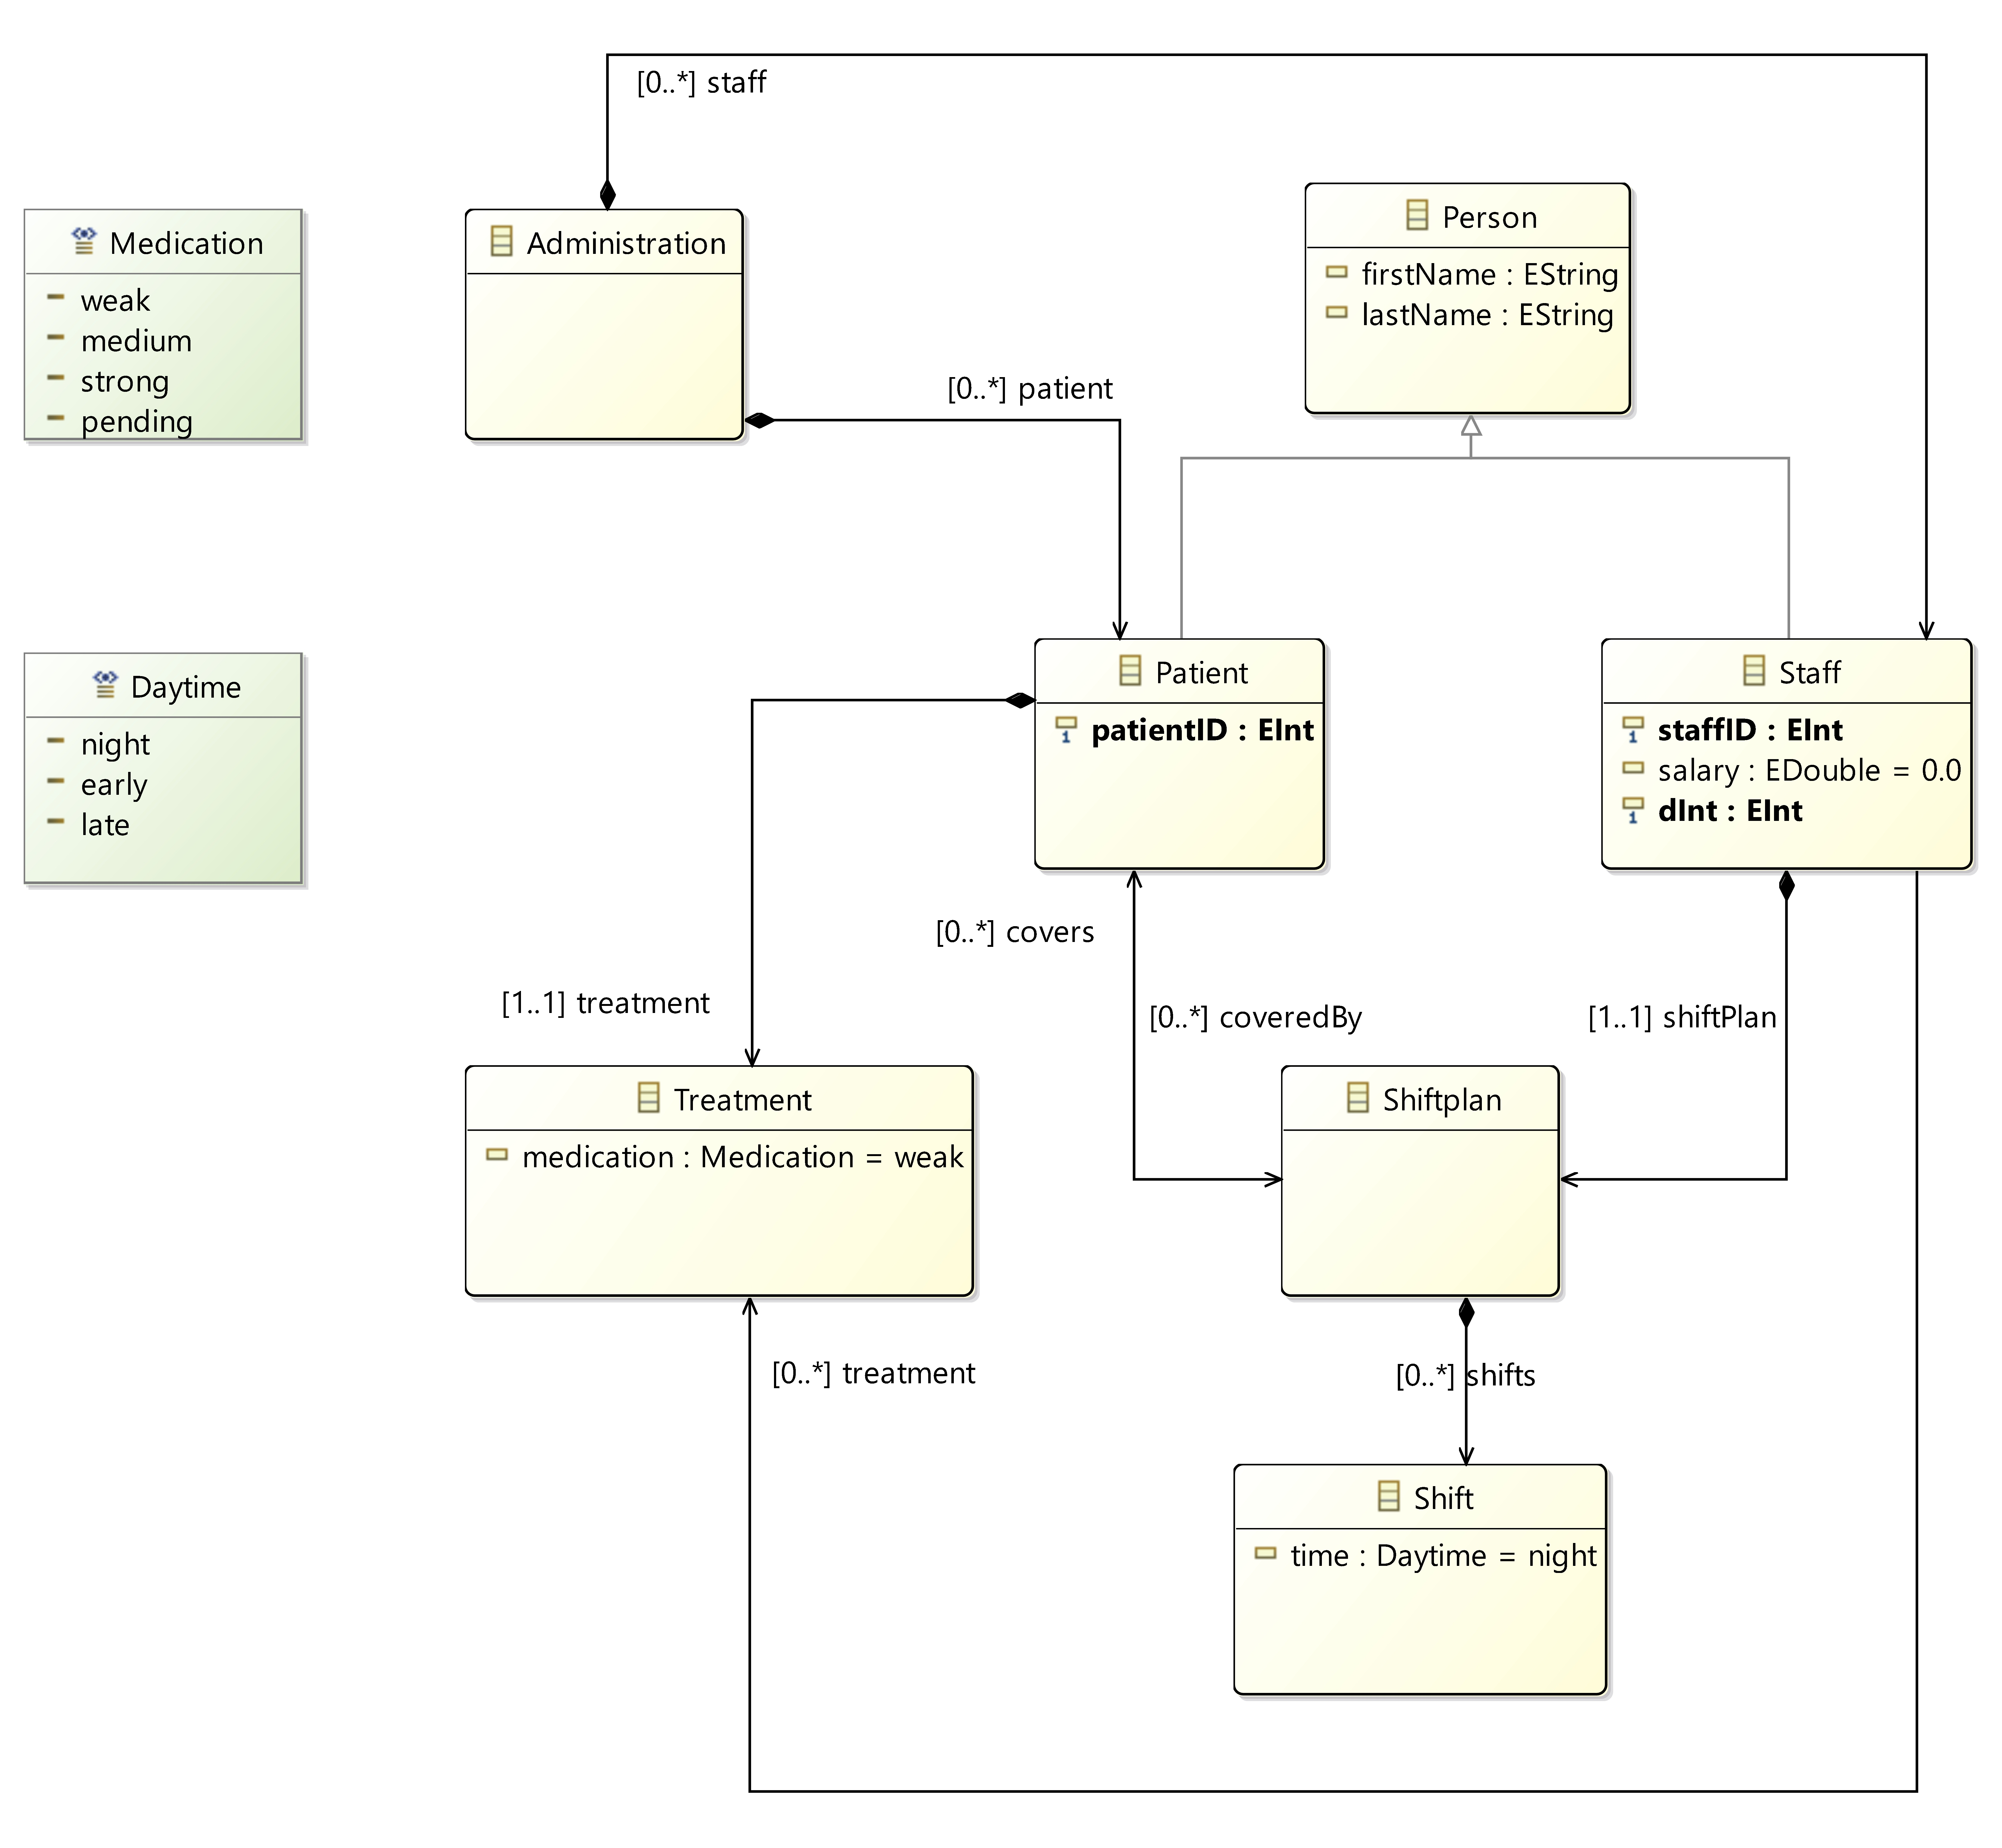
\includegraphics[scale=0.05 ]{pictures/AdministrationExample class diagram.jpg}
    \caption{\centering{Administration model}}
    \label{Administration model}
\end{figure}

\clearpage

For this purpose, we will be creating this new \textbf{administration metamodel} from scratch. If you do not want to exercise the creation of another metamodel yourself, you can skip this part and continue here with the \textbf{creation of a new TGG Project} in the next section.\newline

For our administration metamodel, we need the administration container first. So go ahead and create it \textbf{as we did it for the hospital}.\newline

\textbf{Persons:}

Then we need the persons which we want to cover for our administration. So, the next class you want to create are the \textbf{persons}, who should have a \textbf{first name} and a \textbf{last name} of the type \textbf{EString}.\newline

\textbf{Shifts:}

The two next classes are the \textbf{patients} and the \textbf{staff}, which are of the \textbf{ESuperType} person so both patients and staff members are extended by the persons and have names as well. For the staff, we also want additional information such as the \textbf{staffID}, a \textbf{salary}, and the \textbf{dInt} variable to indicate the department a staff member belongs to. A patient only needs a \textbf{patientID} as an additional attribute. After creating the two classes we need to connect them to the administration by adding a \textbf{staff relation} for the staff and \textbf{patient relation} for the patients.\newline

\textbf{Shiftplans:}

The next classes shiftplan and shift will be responsible for the coverage of the patients. So go ahead and create the class \textbf{Shiftplan} it does not require any attributes. But we want to add a \textbf{relation towards the staff} which ensures every staff member has \textbf{exactly one} shiftPan. Create the relation \textbf{shiftPlan} and set the upper and lower bounds to 1 to fulfill the desired multiplicities. We also want the patients to be covered by the shiftplan. Hence, we need a \textbf{bidirectional relation between the patients and the shift plans}.


The class \textbf{shift} will fill up a shiftPlan with shifts for the respective daytime. The times can be considered via the creation of the \textbf{Daytime Enumeration} with the literals \textbf{night}, \textbf{early}, and \textbf{late} and adding them as an attribute to the shifts class.\newline

\textbf{Medication and Treatment:}

After covering the care throughout the day, the treatment of patients is of importance as well. So, we need to create the \textbf{enumeration Medication} with the following four types: \textbf{weak}, \textbf{medium}, \textbf{strong}, and \textbf{pending}.

Then we have to create a class that includes the medication. Create the class \textbf{Treatment} and a \textbf{medication attribute} that accesses the medication enumeration. The last step we need to do is to \textbf{connect the treatment class to our staff and the patients}. \newline

The created metamodel should be completed now.

\subsection{Creating a TGG project}

%For this section, we will be using the \textbf{branch \textsf{EcoreOnly2}} from our Git repository.

%If you skipped the creation of the metamodel or you are unsure whether your model works correctly, please use this branch of our repository for the next section.\newline

We have now two metamodels containing information that are partly the same and partly different, but how do we connect the two sides and create a consistent triple? As a reminder, a consistent triple consists of three models which are related. The first model of a consistent triple is a so-called \textbf{source model}, which is represented by the hospital model in our case. The second model is the so-called \textbf{target model}, which is the administration model we have created in the previous segment. The third model is the \textbf{correspondence model} which puts the target and source model with each other.\newline

\textbf{Project creation:}

Let us start with creating a new TGG Project to link our hospital metamodel with the administration metamodel. To create a new TGG Project just click on button \ref{item:3} with the \textbf{green rhomb and the folder}. Then proceed with:\newline

\centering

Use the name \textsf{"Hospital2Administration"} → Select option \textsf{"Project with preselected metamodel"}

→ Press \textsf{"next"}

\clearpage

\raggedright

Now you have to select a \textbf{source metamodel} which will be the hospital example in our case. Scroll down through the list of possible options shown in the chart below  and select:\newline

\centering

\textcolor{Blue}{\textsf{platform:/resource/HospitalExample/model/HospitalExample.ecore}}\newline

\raggedright

\begin{figure}[h]
    \centering
    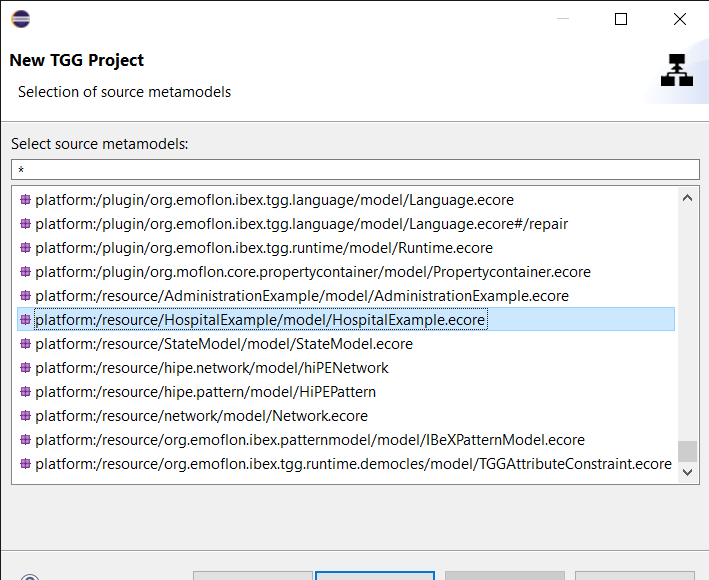
\includegraphics[scale=0.5 ]{pictures/selectSourceModel.png}
    \caption{\centering{Source model selection}}
    \label{Source model selection}
\end{figure}

The second model to select will be our \textbf{target model} and you might have already guessed it we will select our Administration metamodel: \newline

\centering

\textcolor{Blue}{\textsf{platform:/resource/AdministrationExample/model/AdministrationExample.ecore}}\newline

-> Afterwards press \textsf{"Finish"}\newline

\raggedright

Right now, we have a hospital metamodel and an administration metamodel but they are not connected. As a consequence, we need means to create relations between our two metamodels. These relations are defined in the files we will inspect now.

In the source folder you will find the \textbf{tgg package} and in it you will find the \textbf{Schema.tggl} file. This file is the central element linking both the source and the target side since it defines the \textbf{correspondence metamodel} for the connections between both the source and the target side. The correspondence metamodel defined by the Schema.tggl also completes our triple of metamodel graphs.\newline

\textbf{Warning:} Please always start the name of your project with a \textbf{capital letter}. The automatic file generation will not work otherwise.\newline

There are three important parts in the Schema file. Also there are a lot of desired elements missing in the Schema.tggl which will be added throughout the next section. Do not worry we will explain everything in detail and walk you through every step.
\clearpage

\subsection{Writing a TGG schema}

The automatically generated Schema.tggl should look like this:\newline

{\setstretch{1.2}

1\hspace{0.5cm}\textcolor{Purple}{\textit{import}} \textcolor{Orange}{"platform:/resource/AdministrationExample/model/AdministrationExample.ecore"} \textcolor{Purple}{using} HospitalExample \textcolor{Purple}{as} HE

2\hspace{0.5cm}\textcolor{Purple}{\textit{import}} \textcolor{Orange}{"platform:/resource/HospitalExample/model/HospitalExample.ecore"} \textcolor{Purple}{using} AdministrationExample \textcolor{Purple}{as} AE

3\hspace{0.5cm}\textcolor{Purple}{\textit{schema}} Hospital2Administration \{

4\hspace{0.5cm}\colorbox{LightYellow}{\textit{source}} \{

5\hspace{1cm}HospitalExample

6\hspace{0.5cm}\}

7\hspace{0.5cm}\colorbox{LightSalmon}{\textit{target}}\{ 

8\hspace{1cm}AdministrationExample

9\hspace{0.5cm}\} 

10\hspace{0.5cm}\textcolor{Purple}{\textit{correspondence}} \{

11\hspace{0.5cm}\}

12\hspace{0.5cm}\}\newline

}


\textbf{Source and target model:}

First, the Schema.tgg defines the \textbf{source} and the \textbf{target} which was done automatically in our case because we defined the source and target model when we created the project. If you want to start with a blank project you have to do this yourself. You can see this definition in lines 5 and 8 where the \textsf{HospitalExample} metamodel was defined as the source model and the \textsf{AdministrationExample} metamodel was defined as the target model.\newline
Additionally you can define \textbf{aliases}. Those are meant for you to adress your source and target model in the way you want. In the Schema.tggl file you can see those aliases defined by using the keyword \textbf{as} and the name you intend, here \textbf{HE} for HospitalExample and \textbf{AE} for AdministrationExample. In the correspondences we will define on the next page you can see that we use the aliases to specify the model we want to adress instead of the full name.\newline

\textbf{Correspondences:}

The second block consists of the \textbf{correspondences} between our meta models. The connections between our models we have talked previously about are called correspondences and their purpose is to define the elements which are connected. This might be a bit confusing so let us take a look at our example to make things clearer. The very first correspondence we want to create is the correspondence between our hospital and the administration. We can create a correspondence by writing the name of our correspondence and defining which elements on the source and target side should be connected in this correspondence. We recommend using the names of the elements we want to correspond with each other as the \textbf{names for the correspondence} for comprehensibility reasons.\newline

\textbf{Staff and patients:}

Go ahead and write \textsf{Hospital2Administration} within the \textcolor{Purple}{\textit{correspondence}} bracket and \textbf{add curved brackets} to it.
Now we need to choose an element of the source/hospital side we want to correspond with an element on the target/administration side. As the name of the correspondence already indicates we want the \textbf{hospital class} to correspond with the \textbf{administration class} on the target metamodel.

A source element can be added via typing \textsf{src-> <nameOfElement>}. In the case of our hospital, we have to type \textsf{src->Hospital}.

Since we are still missing an element on the target side, we add the administration by writing \textsf{trg->Administration}. Our correspondence metamodel has now one correspondence between the hospital and the administration.\newline

However, we have still more elements we want to correspond with each other. Furthermore we want to connect the \textbf{staff} and the \textbf{patients} of both sides to each other. Let us create the new correspondence \textsf{StaffToStaff} and assign the staff classes of both sides as target and source to this correspondence.\newline

Try coding the \textsf{PatientToPatient} correspondence yourself. For the correspondence between patients, we want to connect the patients on the source side with their respective counterparts on the target side.\newline

\textbf{Doctors and nurses:}

Now we have covered the rather obvious correspondences between our two models, but some classes contain information we want to be present in the other model too. We only have staff members on the target side but we still want to differentiate \textbf{doctors} from \textbf{nurses} there. Since we do know that the doctors and the nurses are related to the staff class on the source side, it makes sense to let the nurses and doctors correspond with the staff on the target side.

Let us create two further \textbf{correspondences} then. Firstly, we need the \textbf{DoctorToStaff} correspondences which ensures a doctor on the source side corresponds with the staff on the target side. Secondly, the nurses should correspond with staff in the same way, and hence we need the \textbf{NurseToStaff} correspondence.\newline

Finally your \textcolor{Purple}{\textit{correspondence}} section should look like this:\newline

{\setstretch{1.2}


10\hspace{0.5cm}\textcolor{Purple}{\textit{correspondence}} \{

11\hspace{1cm}Hospital2Administration\{

12\hspace{1.5cm}\colorbox{LightYellow}{\textit{src->}}HospitalExample.Hospital

13\hspace{1.5cm}\colorbox{LightSalmon}{\textit{trg->}}AdministrationExample.Administration

14\hspace{1cm}\}

15\hspace{1cm}StaffToStaff\{
	
16\hspace{1.5cm}\colorbox{LightYellow}{\textit{src->}}HE.Staff

17\hspace{1.5cm}\colorbox{LightSalmon}{\textit{trg->}}AE.Staff

18\hspace{1cm}\}

19\hspace{1cm}PatientToPatient\{

20\hspace{1.5cm}\colorbox{LightYellow}{\textit{src->}}HE.Patient

21\hspace{1.5cm}\colorbox{LightSalmon}{\textit{trg->}}AE.Patient

22\hspace{1cm}\}

23\hspace{1cm}DoctorToStaff\{

24\hspace{1.5cm}\colorbox{LightYellow}{\textit{src->}}HE.Doctor

25\hspace{1.5cm}\colorbox{LightSalmon}{\textit{trg->}}AE.Staff

26\hspace{1cm}\}

27\hspace{1cm}NurseToStaff\{

28\hspace{1.5cm}\colorbox{LightYellow}{\textit{src->}}HE.Nurse

29\hspace{1.5cm}\colorbox{LightSalmon}{\textit{trg->}}AE.Staff

30\hspace{1cm}\}

31\hspace{0.5cm}\}

}

\clearpage

\subsection{TGG Rules}

Since the ruleset and certain specifications for the triple grammar graph project are quite extensive, we do not want you to create everything by yourself but rather explain to you the ideas behind certain structures. For this reason there are two Hospital2Administration projects. \textbf{Hospital2Administration} is the template you should be using for this part of the tutorial. It contains all of the predefined stuff you need for it and you can just add the new stuff to it. \textbf{Hospital2AdministrationSolution} contains the solution for this part of the tutorial\footnote{Please notice that the packages in the solution projects also contain the string \texttt{solutions}. With this differentiation, you are able to import both projects to the same workspace simultaneously.}.\newline

\textbf{First rule:}

In contrast to the Schema.tgg where we defined the correspondence metamodel for the hospital and the administration, rules are responsible for the \textbf{creation of the actual structure} of our triple grammar graph. You will notice they work similarly to the rules we defined in the graph transformation project. Start with the creation of a new TGG rule in the package \textsf{org.emoflon.ibex.tgg.rules}.\newline

\textbf{Please create this rule in the described way.}\newline

\centering

Click on the package →  Press button \ref{tgg_rule} → Name it \textsf{"HospitalToAdministration"} → \textsf{"Finish"}\newline

\raggedright

\begin{figure}[h]
    \centering
    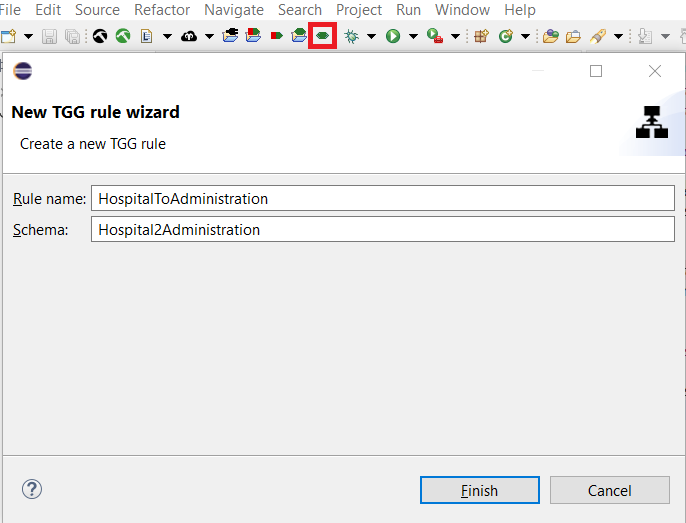
\includegraphics[scale=0.5 ]{pictures/tgg_rule_creation.png}
    \caption{\centering{TGG rule creation}}
    \label{TGG rule creation}
\end{figure}

As we can see the proper schema is assigned automatically, at least if you have selected the right package in your TGG project.\newline

For our first TGG rule, we want to create a connection for the hospital and the administration, as well as the nodes themselves. For this rule, we want a \textbf{hospital node} and a \textbf{reception node} with an \textbf{edge between them} on the source side.

The target side will require the creation of an \textbf{administration node}.

So far, the syntax of our TGG rule is almost the same as in graph transformation projects.\newline

According to the correspondence metamodel that we have defined in the Schema.tgg this rule also needs to consider the correspondence between our hospital node and the administration node. We do this by \textbf{adding a new correspondence} (lines 16 to 20) in the \textcolor{Purple}{correspondence} bracket.

This is similar to the principle of graph transformation rules. We first have define in the ecoremodel what relations different elements in our model have between each other, i.e references.
When creating instances of these elements via the application of a rule we also need to add an instance of those relations explicitly.

\clearpage

Please name the correspondence \textsf{htov} and define its type as \textsf{Hospital2Administration}. This is the correspondence we have created in the Schema.tggl. 

Now we are going to add the hospital node we have created in this rule to the source side and the administration node to the target side.\newline

Finally your rule should look like this: \newline

{\setstretch{1.2}
	
	\hspace{0.5cm}\colorbox{LightYellow}{\textit{source}}\{ 
	
	\hspace{1cm}\textcolor{LimeGreen}{[+] h:HE.Hospital\{}
	
	\hspace{1.5cm}\textcolor{LimeGreen}{[+] -reception->r}
	
	\hspace{1cm}\textcolor{LimeGreen}{\}}
	
	\hspace{1cm}\textcolor{LimeGreen}{[+] r:HE.Reception\{}
	
	\hspace{1cm}\}
	
	\hspace{0.5cm}\}
	
	\hspace{0.5cm}\colorbox{LightSalmon}{\textit{target}}\{
	
	\hspace{1cm}\textcolor{LimeGreen}{[+] v:AE.Administration}
	
	\hspace{0.5cm}\}
	
	\hspace{0.5cm}\textcolor{Purple}{\textit{correspondence}}\{
	
	\hspace{1cm}\textcolor{LimeGreen}{[+] htov:HospitalToAdministration\{}
	
	\hspace{1.5cm}\colorbox{LightYellow}{\textit{src->}}\textcolor{LimeGreen}{h}
	
	\hspace{1.5cm}\colorbox{LightSalmon}{\textit{trg->}}\textcolor{LimeGreen}{v}
	
	\hspace{1cm}\}
	
	\hspace{0.5cm}\}
	
	\hspace{0.5cm}\textcolor{Purple}{\textit{attributeConditions}}\{
	
	\hspace{0.5cm}\}\newline
	
}



\begin{figure}[h]
    \centering
    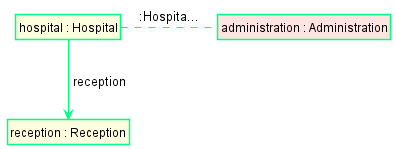
\includegraphics[scale=0.5 ]{pictures/h2a.png}
    \caption{\centering{PlantUML visualization HospitalToAdministration}}
    \label{TGG rule creation}
\end{figure}

\textbf{Note on the visualization}:

On the left side, we see our target side which creates the hospital and the reception and on the right side, we can see a new administration. The dotted line between the hospital and administration stands for the correspondence between the two models.\newline

Since you now have a grasp of how to create a rule let us take a step back and recapitulate its function. The rule creates a consistent triple consisting of the hospital and the reception nodes on the source side, the administration node on the target side, and their connection to each other in form of the correspondence. In other words, whenever we create a hospital and a reception on the source side, our correspondence requires the creation of an administration on the target side.

\clearpage

\textbf{Departments and rooms:}

The next two rules we will create are the rules for the departments and the rooms. 
The department rule creates a department with the respective edge to the hospital and works just as the departmentRule in the GT project. This rule allows the creation of a department if we already created a hospital node in our project. 

So go ahead and create a new tgg rule with the name \textsf{DepartmentRule} for which we need to add the following contents:\newline

{\setstretch{1.2}
	
	\hspace{0.5cm}\textcolor{Purple}{\textit{rule}} \textcolor{black}{DepartmentRule} \{
	
	\hspace{0.5cm}\colorbox{LightYellow}{\textit{source}} \{ 
	
	\hspace{1cm}\textcolor{black}{[=] h : HE.Hospital\{}
	
	\hspace{1.5cm}\textcolor{LimeGreen}{[+] -department->d}
	
	\hspace{1cm}\textcolor{LimeGreen}{\}}
	
	\hspace{1cm}\textcolor{LimeGreen}{[+] d : HE.Department\{}
	
	\hspace{1cm}\}
	
	\hspace{0.5cm}\}
	
	\hspace{0.5cm}\textcolor{black}{\colorbox{LightSalmon}{\textit{target}}} \{
	
	\hspace{0.5cm}\}
	
	\hspace{0.5cm}\textcolor{Purple}{\textit{correspondence}} \{
	
	\hspace{0.5cm}\}
	
	\hspace{0.5cm}\textcolor{Purple}{\textit{attributeConditions}} \{
	
	\hspace{1cm}\textcolor{black}{Hospital2AdministrationLibrary.incrementingDepartmentID(d.dID)}
	
	\hspace{1cm}\textcolor{black}{Hospital2AdministrationLibrary.setDefaultNumber(d, 10)}
	
	\hspace{0.5cm}\}
	
	\}





\textbf{Note:}

We will explain the \textcolor{Purple}{attributeConditions} section later on. Please just copy these sections for now.\newline

\textbf{Please try to code the \textsf{RoomRule} yourself}.\newline

For this rule want to add a \textbf{room node} in case we have a department and assign the \textbf{default capacity} of that room to 4.

It should look like this in the end:\newline

{\setstretch{1.2}
	
	\hspace{0.5cm}\textcolor{Purple}{\textit{rule RoomRule}} \{
	
	\hspace{0.5cm}\colorbox{LightYellow}{\textit{source}} \{ 
	
	\hspace{1cm}\textcolor{black}{[=] d:HE.Department\{}
	
	\hspace{1.5cm}\textcolor{LimeGreen}{[+] -rooms->ro}
	
	\hspace{1cm}\textcolor{LimeGreen}{\}}
	
	\hspace{1cm}\textcolor{LimeGreen}{[+] ro:HE.Room\{}
	
	\hspace{1.5cm} .capacity:=4;
	
	\hspace{1cm}\textcolor{LimeGreen}{\}}
	
	\hspace{0.5cm}\}
	
	\hspace{0.5cm}\textcolor{black}{\colorbox{LightSalmon}{\textit{target}}} \{
	
	\hspace{0.5cm}\}
	
	\hspace{0.5cm}\textcolor{Purple}{\textit{correspondence}} \{
	
	\hspace{0.5cm}\}
	
	\hspace{0.5cm}\textcolor{Purple}{\textit{attributeConditions}} \{
	
	\hspace{0.5cm}\}
	\par
}


As you can see, we are only operating on the source side of our consistent triple since we do not have and do not need a correspondence for these elements on the target side because these elements are not present on the administration side. \newline

\clearpage

\textbf{Abstract rules:}

Let us continue with the remaining rules since we are still lacking the personnel and the patients. Look at the \textsf{StaffToStaffRule} which is already present in your Java project. Its visualization is shown in the chart below.

For this rule, we assume that a hospital node, at least one department node, an administration node and the correspondence between source and target side exist.

Then we want to create a staff node and its respective connections on the source side. When creating a staff node on the target side we also want to connect them to the target side by creating the \textsf{StaffToStaff} \textbf{correspondence} and the staff for the target side itself.

Upon creating a staff member on the target side, we also want to assign them a shift plan and a shift.

\begin{figure}[h]
    \centering
    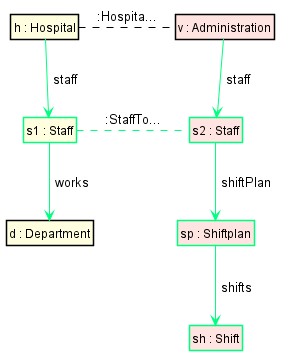
\includegraphics[scale=0.6 ]{pictures/StaffToStaffRule.png}
    \caption{\centering{PlantUML visualization StaffToStaffRule}}
    \label{TGG rule creation}
\end{figure}

You probably have noticed the keyword \textcolor{Purple}{abstract} in the definition of this rule. Similar to \textbf{abstract} rules from graph transformations this means that this rule cannot be applied directly.\newline

\textbf{Extending abstract rules:}

You might also wonder how we are going to distinguish doctors from nurses in the administration view. That is the part where the \textsf{DoctorToStaff} and \textsf{NurseToStaff} \textbf{correspondences} that we have created previously come into play. With those we have established a correspondence between doctors and nurses on the source side to staff on the target side.

This requires a further extension of our Staff rule which can be added just below the \textsf{StaffToStaffRule}. The keyword for the further specification of an existing rule in TGG is \textcolor{Purple}{refines} which needs to be added after the name of the rule. If you remember from the GT part of our tutorial the keyword \textcolor{Purple}{refines} works similar to the concept of inheritance in Java. We reduce redundancies for the new rules because they inherit the elements defined in the \textsf{StaffToStaffRule} as well.
For the creation of the DocToStaff rule, which can be done in the present StaffToStaff rule, we need to add a staff node of the type doctor on our \colorbox{LightYellow}{\textit{source}} side and a new staff node on the \colorbox{LightSalmon}{\textit{target}} side. \newline

{\setstretch{1.2}

1\hspace{0.5cm}\textcolor{Purple}{\textit{rule}} DocToStaffRule \textcolor{Purple}{\textit{refines}} StaffToStaffRule

2\hspace{0.5cm}\colorbox{LightYellow}{\textit{source}}\{

3\hspace{1cm}\textcolor{LimeGreen}{[+] s1d:HE.Doctor}

4\hspace{0.5cm}\}

5\hspace{0.5cm}\colorbox{LightSalmon}{\textit{target}}\{

6\hspace{1cm}\textcolor{LimeGreen}{[+] s2d:AE.Staff}

7\hspace{0.5cm}\}

8\hspace{0.5cm}\textcolor{Purple}{\textit{correspondence}}\{

9\hspace{0.5cm}\}

10\hspace{0.42cm}\textcolor{Purple}{\textit{attributeConditions}}\{

11\hspace{1cm}Hospital2AdministrationLibrary.doctorsalary(s2.salary)

12\hspace{0.5cm}\}\newline

}

\clearpage

The \textsf{NurseToStaffRule} can be created similarly. Please try it yourself before having a look at the syntax below. Change the type of staff member accordingly and adjust the attribute condition to \textsf{nursesalary}.\newline

{\setstretch{1.2}
	
	1\hspace{0.5cm}\textcolor{Purple}{\textit{rule}} NurseToStaffRule \textcolor{Purple}{\textit{refines}} StaffToStaffRule
	
	2\hspace{0.5cm}\colorbox{LightYellow}{\textit{source}}\{
	
	3\hspace{1cm}\textcolor{LimeGreen}{[+] s1n:HE.Nurse}
	
	4\hspace{0.5cm}\}
	
	5\hspace{0.5cm}\colorbox{LightSalmon}{\textit{target}}\{
	
	6\hspace{1cm}\textcolor{LimeGreen}{[+] s2n:AE.Staff}
	
	7\hspace{0.5cm}\}
	
	8\hspace{0.5cm}\textcolor{Purple}{\textit{correspondence}}\{
	
	9\hspace{0.5cm}\}
	
	10\hspace{0.42cm}\textcolor{Purple}{\textit{attributeConditions}}\{
	
	11\hspace{1cm}Hospital2AdministrationLibrary.nursesalary(s2.salary)
	
	12\hspace{0.5cm}\}\newline
	
}



\begin{figure}[h]
    \centering
    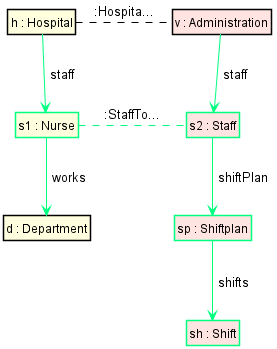
\includegraphics[scale=0.65 ]{pictures/NurseToStaffRule.png}
    \caption{\centering{Visualization of NurseToStaffRule. DocToStaffRule is similar with changed staff type.}}
    \label{NurseToStaffRule}
\end{figure}

\textbf{Shiftplan rule:}

The next function we want to cover is the shift plans. In the \textsf{ShiftplanRule}, we want to add an edge on the target side to make sure a patient is covered by a shift plan. So let us start by creating the new rule \textsf{ShiftPlanRule}.\newline

First, we want to make that rule \textbf{abstract} because as we have defined it in the GT part of our tutorial the coverage of patients via doctors and nurses works differently. While doctors are assigned to a patient directly, nurses cover patients indirectly with the rooms they are responsible for.

We require patient and staff nodes on the source side while having a staff, shift, shift plan and a patient node on the target side. Furthermore this shift plan has to be related to the specific staff and shift nodes via an edge.

For the patient node in our administration model, we want to add an edge to the shift plan to indicate a patient is covered in that shift plan.

In the last step for this rule, we need to define the \textbf{correspondences} with patients and staff members between the source and the target side. Since we have all elements on both sides defined this step should be pretty forward.\newline

You can look at the complete rule on the next page.

\clearpage

{\setstretch{1.2}

1\hspace{0.5cm}\textcolor{Purple}{\textit{abstract}} \textcolor{Purple}{\textit{rule}} ShiftplanRule\{ 
	
	2\hspace{0.5cm}\textcolor{black}{\colorbox{LightYellow}{\textit{source}}} \{ 
	
	3\hspace{1cm}[=] p1:HE.Patient\{
		
	4\hspace{1cm}\}
		
	5\hspace{1cm}[=] s1:HE.Staff\{
		
	6\hspace{1cm}\}
		
	7\hspace{0.5cm}\}
		
	8\hspace{0.5cm}\colorbox{LightSalmon}{\textit{target}} \{ 
		
	9\hspace{1cm}[=] s2:AE.Staff\{
			
	10\hspace{1.5cm}[=] -shiftPlan->sp
			
	11\hspace{1cm}\}
			
	12\hspace{1cm}[=] sp:AE.Shiftplan\{
			
	13\hspace{1.5cm}[=] -shifts->sh
			
	14\hspace{1cm}\}
			
	15\hspace{1cm}[=] sh:AE.Shift\{
			
	16\hspace{1cm}\}
			
	17\hspace{1cm}[=] p2:AE.Patient\{
			
	18\hspace{1.5cm}\textcolor{LimeGreen}{[+] -coveredBy->sp}
			
	19\hspace{1cm}\}
			
	20\hspace{0.5cm}\}
			
	21\hspace{0.5cm}\textcolor{Purple}{\textit{correspondence}} \{ 
			
	22\hspace{1cm}[=] pToP:PatientToPatient\{
				
	23\hspace{1.5cm}\colorbox{LightYellow}{src}->p1
				
	24\hspace{1.5cm}\colorbox{LightSalmon}{trg}->p2
				
	25\hspace{1cm}\}
				
	26\hspace{1cm}[=] sToS:StaffToStaff\{
				
	27\hspace{1.5cm}\colorbox{LightYellow}{src}->s1
				
	28\hspace{1.5cm}\colorbox{LightSalmon}{trg}->s2
				
	29\hspace{1cm}\}
				
	30\hspace{0.5cm}\}
				
	31\hspace{0.5cm}\}


}

\textbf{Specific shiftplans:}

For this case, we also need differentiation between doctors and nurses, due to the different paths towards the coverage of a patient. Hence, we need two more rules.

These are already given in your project. You can look at the respective visualization of the \textsf{DoctorShiftplanRule} and the \textsf{NurseShiftplanRule} in your project: \newline

\begin{figure}[h]
    \centering
    
    \begin{subfigure}[b]{0.3\textwidth}
    
    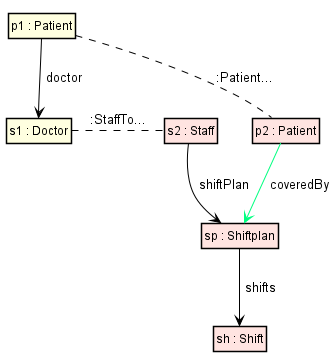
\includegraphics[scale=0.45 ]{pictures/DocShiftplanRule.png}
    \caption{\centering{Visualization of DocShiftplanRule}}
    \label{DocShiftplanRule}
    
    \end{subfigure}\hspace{2cm}
    \begin{subfigure}[b]{0.3\textwidth}
    
    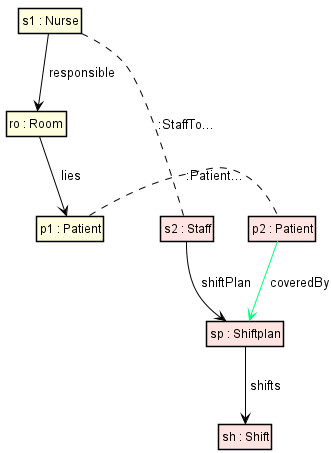
\includegraphics[scale=0.45 ]{pictures/nurseShiftPlan.png}
    \caption{\centering{Visualization of NurseShiftplanRule}}
    \label{NurseShiftplanRule}
    
    \end{subfigure}
    
\end{figure}

\clearpage

\textbf{Rules regarding patients:}

Now that we have covered the staff and their respective shifts, we need to handle the patients. 

The \textbf{abstract} \textsf{PatientToPatientRule} adds patients and the required correspondences for further rules.

This rule is already given in the project and you might want to take a look at it. The visualization is shown in the chart below:

\begin{figure}[h]
    \centering
    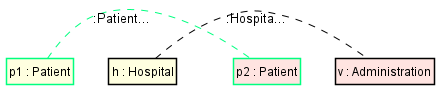
\includegraphics[scale=0.65 ]{pictures/patientToPatient.png}
    \caption{\centering{Visualization of PatientToPatientRule}}
    \label{PatientToPatientRule}
\end{figure}

As you might have noticed we are adding two correspondences to our model which are independent from each other. This requires us to add two rules extending the \textsf{\textit{PatientToPatient}} rule to fit the patients into our hospital view.

For the first rule, we assume that our patients are waiting in the reception until they are moved to a room where they are treated. So, we want to create the rule \textsf{PatientInReception} where we require the context of the hospital node, the edge towards the reception and the reception node on the source side. Additionally, we require the context of the administration node and the \textsf{HospitalToAdministration} correspondence between the hospital node and the administration node. 

Regarding the creation of nodes and edges, we want to add a patient node and a \textsf{waits} edge from the reception to the patient on the source side.

For the target side, we want to create the patient node and its respective edge from the administration towards the patient node.\newline

\textbf{Please try creating this rule yourself, the syntax can be found below:}\newline

{\setstretch{1.2}

1\hspace{0.5cm}\textcolor{Purple}{\textit{rule}} PatientInReception \textcolor{Purple}{\textit{refines}} PatientToPatient \{

2\hspace{0.5cm}\colorbox{LightYellow}{\textit{source}} \{ 

3\hspace{1cm}\textcolor{LimeGreen}{[+] p1r : HE.Patient}

4\hspace{1cm}[=] hr:HE.Hospital\{

5\hspace{1.5cm}[=] -reception->r

6\hspace{1cm}\}

7\hspace{1cm}[=] r:HE.Reception\{

8\hspace{1.5cm}\textcolor{LimeGreen}{[+] -waits->p1}

9\hspace{1cm}\}

10\hspace{0.5cm}\}

11\hspace{0.5cm}\colorbox{LightSalmon}{\textit{target}} \{

12\hspace{1cm}\textcolor{LimeGreen}{[+] p2r : AE.Patient}

13\hspace{1cm}[=] vr:AE.Administration\{

14\hspace{1.5cm}\textcolor{LimeGreen}{[+] -patient->p2}

15\hspace{1cm}\}

16\hspace{0.5cm}\}

17\hspace{0.5cm}\textcolor{Purple}{\textit{correspondence}} \{
	
18\hspace{1cm}[=] htovr:HospitalToAdministration\{

19\hspace{1.5cm}\colorbox{LightYellow}{\textit{src->}}hr
			
20\hspace{1.5cm}\colorbox{LightSalmon}{\textit{trg->}}vr

21\hspace{1cm}\}

22\hspace{0.5cm}\}

23\hspace{0.5cm}\textcolor{Purple}{\textit{attributeConditions}} \{

24\hspace{0.5cm}\}

25\hspace{0.5cm}\}

}

\clearpage

The second rule \textsf{PatientInRoom} is already given in your project. This rule adds the \textsf{lies} edge from the context node \textsf{room} to the node \textsf{patient}.\newline

Its visualization is depicted in the chart below:

\begin{figure}[h]
    \centering
    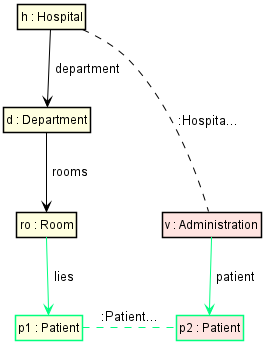
\includegraphics[scale=0.65 ]{pictures/PatientInRoomRule.png}
    \caption{\centering{Visualization of PatientInRoomRule}}
    \label{PatientInRoomRule}
\end{figure}

\textbf{NurseToRoomRule:}

The last remaining rule is the \textsf{NurseToRoomRule}, where we add the edge from the nurse node to the room node according to the assumptions in our metamodel. The rule is also given in your project and the visualization is depicted in the chart below:

\begin{figure}[h]
    \centering
    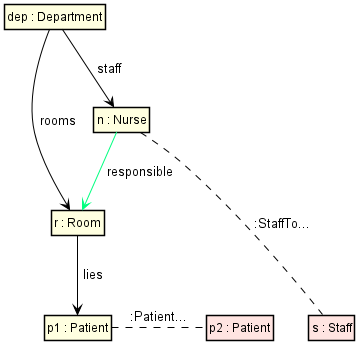
\includegraphics[scale=0.65 ]{pictures/NurseToRoomRule.png}
    \caption{\centering{Visualization of PatientInRoomRule}}
    \label{PatientInRoomRule}
\end{figure}

After creating the rules for the infrastructure and the persons in the hospital you should have a grasp of the concept of creating rules for triple graph grammars and the way they are working. So let us continue with another important function we have skipped previously, the \textbf{attribute conditions}. 

\clearpage

\subsection{Attribute Conditions}

In this chapter we will be covering \textbf{attribute conditions}. Attribute conditions can be used to assign meaningful values to attributes when creating a coherent graph triplet. They can also modify already set attribute values of an existing target and source graph pair to synchronize them.

They will be applied when their corresponding rule is.\newline

You have already seen how to invoke them in the previous chapters:

{\setstretch{1.2}

\hspace{0.5cm}...

\hspace{0.5cm}\textcolor{Purple}{\textit{attributeConditions}} \{

\hspace{1cm}Hospital2AdministrationLibrary.incrementingDepartmentID(department.dID)

\hspace{1cm}Hospital2AdministrationLibrary.setDefaultNumber(department.maxRoomCount, \textcolor{Grey}{10})

\hspace{0.5cm}\} \newline

}

To introduce you to the inner workings of attribute conditions we will have a look a the pre-defined condition \textsf{setDefaultNumber(variableNumber:EDouble, defaultNumber:EDouble)}.\newline

Please, go to \textbf{line 75} in the file \textbf{DefaultAttributeConditionLibrary} in the shown location:

\begin{figure}[h]
    \centering
    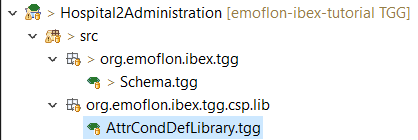
\includegraphics[scale=0.65 ]{pictures/locSetDefaultNumber.png}
    \caption{\centering{Location of \textsf{setDefaultNumber}}}
    \label{setDefaultNumber}
\end{figure}

This file contains the library of predefined attribute conditions. Let us inspect the setDefaultNumber condition which was used previously. This attribute condition ensures that an attribute value is set to a defined default number if it is unset. \newline

\textbf{Control flow:}

Attribute conditions in general
use a control flow that will be defined and is implemented as a \textbf{switch case}. Each case condition is made up by \textbf{all valid combinations of the bounding states} of referenced attribute values, i.e the input parameters.\newline

An attribute can be \textbf{free} meaning that there is no value assigned to it. This will be represented as "\textcolor{Purple}{F}" in the condition.

The other option is that the attribute is \textbf{bonded} which means that it already has a set value. This will be represented as "\textcolor{Purple}{B}" in the condition.

These cases will be defined in the definition of the attribute condition.\newline

Note that there are two different sets of cases for the two application scenarios:

\begin{itemize}
    \item\textcolor{Purple}{\textit{sync}}: Keeping two existing graphs synchronized. [\textcolor{Purple}{ F F } ... \textcolor{Purple}{ F}] is not available since unset values don't need to be synchronized.
    \item\textcolor{Purple}{\textit{gen}}: Generation of a new graph pair.
\end{itemize}

\clearpage

\textbf{Pre-defined conditions:}

Let's have a look at the definition of \textsf{setDefaultNumber}:\newline

{\setstretch{1.2}

75\hspace{0.5cm}setDefaultNumber(variableNumber:EDouble, defaultNumber:EDouble) \{

76\hspace{1cm}\textcolor{Purple}{\textit{sync}} \{ [\textcolor{Purple}{\textit{B B}}], [\textcolor{Purple}{\textit{F B}}] \}

77\hspace{1cm}\textcolor{Purple}{\textit{gen}} \{ [\textcolor{Purple}{\textit{B B}}], [\textcolor{Purple}{\textit{F B}}], [\textcolor{Purple}{\textit{F F}}] \}

78\hspace{0.5cm}\}\newline

}

Because this condition is pre-defined the effects of each case are already implemented. If an attribute has no value and is perceived as free, it would be assigned the \textsf{defaultNumber:EDouble} we defined in the attribute condition of our rule. If the \textsf{variableNumber:EDouble} is already set and hence bound, the bound variableNumber will be kept.

Note that there is no case [\textcolor{Purple}{B F}] because a default value has to be specified for this to work.\newline

You can find a comprehensive list of the predefined attribute conditions and a short explanation of each condition in the \textbf{appendix}.\newline

\textbf{User-defined conditions:}

To create a user-defined attribute condition you have to define your own \textbf{library}. We will call it \textbf{Hospital2AdministrationLibrary}. Let us start by inspecting the \textsf{incrementingDepartmentID} which is already given:\newline

{\setstretch{1.2}

88\hspace{0.5cm}incrementingDepartmentID(id:EInt) \{
	
89\hspace{1cm}\textcolor{Purple}{\textit{sync}} \hspace{0.3cm}\{ [\textcolor{Purple}{\textit{B}}], [\textcolor{Purple}{\textit{F}}] \}
		
90\hspace{1cm}\textcolor{Purple}{\textit{gen}} \hspace{0.3cm}\{ [\textcolor{Purple}{\textit{F}}] \}
		
91\hspace{0.5cm}\}\newline
}

A Library is defined by the keyword \textcolor{Purple}{library} followed by the \textbf{name} of the library. You can define as many libraries as you want.

In our case, we want to modify the ID of a department. The different boundary states are defined in the curved brackets just like in the predefined attribute conditions.\newline

%/*Now head to the \textsf{.constraints.custom.hospital2administration} package and open up the \textsf{UserDefined\_incrementingDepartmentID}. Which should look like this: \newline
%
%{\setstretch{1.2}
%
%1\hspace{0.5cm}\textcolor{Purple}{public class}
%UserDefined\_incrementingDepartmentID \textcolor{Purple}{extends} RuntimeTGGAttributeConstraint
%
%2\hspace{0.5cm}\{\hspace{0.5cm}	\textcolor{Purple}{private static int} \textcolor{Blue}{\textit{idIncrement}} = 1;
%
%3\hspace{1cm}\textcolor{Grey}{@Override}
%
%4\hspace{1cm}\textcolor{Purple}{public void} solve() \{
%
%5\hspace{1.5cm}\textcolor{Purple}{if} (\textcolor{Blue}{variables}.size() != 1)
%
%6\hspace{2cm}\textcolor{Purple}{throw new} RuntimeException("\textcolor{Blue}{The CSP -INCREMENTINGDEPARTMENTID- needs exactly 1 variables}");
%
%7
%
%8\hspace{1.5cm}RuntimeTGGAttributeConstraintVariable \textcolor{Tan}{v0} = \textcolor{Blue}{variables}.get(0);
%
%9\hspace{1.5cm}String \textcolor{Tan}{bindingStates} = getBindingStates(\textcolor{Tan}{v0});
%
%10
%
%11\hspace{1.5cm}\textcolor{Purple}{switch}(\textcolor{Tan}{bindingStates}) \{
%
%12\hspace{1.5cm}\textcolor{Purple}{case} "\textcolor{Blue}{F}":
%
%13\hspace{2cm}\textcolor{Tan}{v0}.bindToValue(\textcolor{Blue}{\textit{idIncrement}}++);
%
%14\hspace{2cm}setSatisfied(\textcolor{Purple}{true});
%
%15\hspace{2cm}\textcolor{Purple}{break};
%
%16\hspace{1.5cm}\textcolor{Purple}{case} "\textcolor{Blue}{B}":
%
%17\hspace{2cm}setSatisfied(\textcolor{Purple}{true});
%
%18\hspace{2cm}\textcolor{Purple}{return};
%
%19\hspace{1.5cm}\textcolor{Purple}{default}: \textcolor{Purple}{throw new} UnsupportedOperationException("\textcolor{Blue}{This case in the constraint has not been implemented yet: }" + \textcolor{Tan}{bindingStates});
%
%}

%\clearpage
%
%In line 2 we define the initial value of our department ID in the static variable \textsf{idIncrement}. Which will be incremented later on in the switch statement in lines 13 to 14.
%
%If the department ID is free which is given as the parameter \textsf{id} in our attribute condition we switch to the \textcolor{Purple}{case} \textsf{"\textcolor{Purple}{F}"} and bind the ID to the value of the \textsf{idIncrement} variable. Afterwards we increasing this variable to give each department an unique ID.
%
%In the next line, we set the boolean variable \textsf{setSatisfied} to \textsf{true} to fulfill the requirement for our runtime variable.
%
%For the second \textcolor{Purple}{case} \textsf{“\textcolor{Purple}{B}”} we just set the setSatisfied value to true, since a department already has an ID and does not need one. \newline

Be aware that after the application of an attribute condition all involved attributes have to be \textbf{bound}.\newline

Maybe we should practice a bit by creating a fresh user-defined attribute condition. Our rooms also have IDs that we want to assign identically to the departmentIDs. Start by defining the attribute constraint \textsf{incrementingRoomID} in the \textsf{schema.tgg}. Its definition should look very similar:\newline

{\setstretch{1.2}

108\hspace{0.5cm}incrementingRoomID(id:EInt)

109\hspace{0.5cm}\{
	
110\hspace{1cm}\textcolor{Purple}{\textit{sync}}\{[\textcolor{Purple}{B}],[\textcolor{Purple}{F}]\}
		
111\hspace{1cm}\textcolor{Purple}{\textit{gen}}\{[\textcolor{Purple}{F}]\}
		
112\hspace{0.5cm}\}\newline

}

Please \textbf{build} the project by pressing either the \textbf{black or the green hammer button} \ref{item:0} in the eMoflon Toolbar. Once you refresh your project folder you can see that the new attribute condition was created automatically and tucked into our project by eMoflon.

\clearpage

\textbf{Complex conditions:}

To further get to know user-defined attribute constraints let us look at the \textsf{UserDefined\_nametoname.Java} file which is a rather complex condition and already given in our project. As you can see in the schema.tgg the number of different boundary states has increased notably since we are handling more parameters. \newline

{\setstretch{1.2}

82\hspace{0.45cm}nametoname(separator:EString, leftWord:EString, rightWord:EString, result:EString) \{

83\hspace{1cm}\textcolor{Purple}{\textit{sync}}\{ [\textcolor{Purple}{\textit{B B B B}}], [\textcolor{Purple}{\textit{B B B F}}], [\textcolor{Purple}{\textit{B B F B}}], [\textcolor{Purple}{\textit{B F F B}}], [\textcolor{Purple}{\textit{B F B B}}]\}
		
84\hspace{1cm}\textcolor{Purple}{\textit{gen}}\{ [\textcolor{Purple}{\textit{B B B B}}] , [\textcolor{Purple}{\textit{B B B F}}], [\textcolor{Purple}{\textit{B B F B}}], [\textcolor{Purple}{\textit{B F F B}}], [\textcolor{Purple}{\textit{B F B B}}], [\textcolor{Purple}{\textit{B F B F}}], [\textcolor{Purple}{\textit{B B F F}}], [\textcolor{Purple}{\textit{B F F F}}]\}

85\hspace{0.45cm}\} \newline
	
}

We should start by explaining the purpose of this attribute constraint. If you compare the name attributes of the patients and staff members in the hospital metamodel with the name attribute of the Person class in the administration metamodel, you will notice that the name attributes on the administration side are split up in first and last name. This specification forces us to split up the full name consisting of first and last name on the hospital side into two attributes if we want to propagate the name information from the hospital side to the administration side or concatenate two names if we want to execute the opposite operation. This leads to the four parameters we need for the attribute constraint.

The \textsf{separator:EString} defines the character we are using to distinguish first from last name in case both are in the same attribute. The \textsf{leftWord:EString} will define the first name while \textsf{rightWord:EString} will be handling the last name. The \textsf{result:EString} combines the three previous Strings to one String. \newline

\clearpage

%If you open the java file of the attribute constraint you can see two arrays with sample names which we are using to generate a random first and last name whenever we invoke the attribute constraint, and the name attributes are not set yet:\newline
%
%{\setstretch{1.2}
%
%25\hspace{0.5cm}\textcolor{Purple}{case} \textcolor{Blue}{"BFFF"}:
%
%26		  		
%
%27\hspace{1cm}String \textcolor{Tan}{firstName} = firstNames[\textcolor{Tan}{random}.nextInt(\textcolor{Tan}{firstNames}\textcolor{Blue}{.length})];
%
%28\hspace{1cm}\textcolor{Tan}{v1}.bindToValue(\textcolor{Tan}{firstName});
%
%29\hspace{1cm}String \textcolor{Tan}{lastName} = \textcolor{Tan}{lastNames}[\textcolor{Tan}{random}.nextInt(\textcolor{Tan}{lastNames}\textcolor{Blue}{.length})];
%
%30\hspace{1cm}\textcolor{Tan}{v2}.bindToValue(\textcolor{Tan}{lastName});
%
%31\hspace{1cm}\textcolor{Tan}{v3}.bindToValue(\textcolor{Tan}{firstName} + \textcolor{Tan}{v0}.getValue() + \textcolor{Tan}{lastName});
%
%32\hspace{1cm}setSatisfied(\textcolor{Purple}{true});	
%
%33\hspace{1cm}\textcolor{Purple}{break}; \newline
%
%}
%
%For the case above we want a bound separator character which is a blank space in our case. Then we select a random first name from our first name array and bind its value to the runtime variable \textsf{v1} which represents the \textbf{leftWord}.
%
%The same is done for the last name.
%
%\textsf{v3} is the result of combining the values of the previous runtime variables.\newline
%
%As you can see the user-defined constraints are a powerful way to create constraints that are not covered by our predetermined library.

\subsection{Running the TGG Project}

Now that we have finally defined all the elements and their respective correspondences of our models it is time to get back to our primary goal for this part of the tutorial. The generation of a consistent triple and its consistency maintenance.\newline

As a short reminder: A consistent triple includes the source model, a correspondence model, and a target model. Once information changes in one model we want to propagate the information to the other models to achieve consistency. eMoflon provides a different set of Java applications for this purpose and we will go through the important ones step by step. \newline

Open the package \textsf{org.emoflon.ibex.tgg.run.hospital2administration} and take a look at the different java applications you can see in the chart below:

\begin{figure}[h]
    \centering
    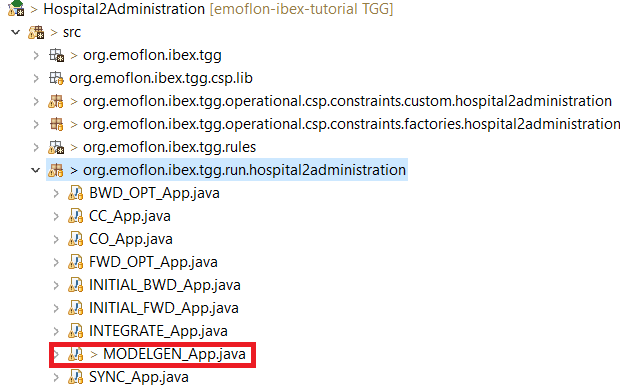
\includegraphics[scale=0.65 ]{pictures/modelGENApp.png}
    \caption{\centering{run.hospital2administration package}}
    \label{setDefaultNumber}
\end{figure}

The first operation we are interested in is the \textit{\textsf{MODELGEN\_APP.java}} which is marked above. Let us start exploring this feature by \textbf{running} it in our java project. Please \textbf{refresh} the project folder afterwards.\newline

Once you open the \textsf{instances} folder it should look like this:

\begin{figure}[h]
    \centering
    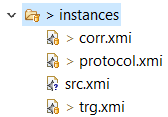
\includegraphics[scale=0.85 ]{pictures/instances.png}
    \caption{\centering{instances folder}}
    \label{setDefaultNumber}
\end{figure}

\textbf{Model generation via MODELGEN:}

The \textsf{MODELGEN\_APP} generates a consistent triple according to our rule sets without any preexisting models. It generates a hospital model, an administration target model, and the correspondence model for the connections between our source and target model.\newline

By opening the \textsf{src.xmi} you can take a look a the final model instance. You should see patients waiting in the reception or being assigned to their rooms as well as the staff members within their departments. Nurses for example which should be covering a room with patients. Look at the \textsf{trg.xmi} and you will notice that we have the same patients and staff members in this model instance. But here we focus on the shifts of the latter and treatments we assigned to their patients.

A model generator might also be helpful for testing purposes, especially scalability testing that requires large models. \newline

\textbf{Other running options:}

Let us explore the other run options as well. Although we are mainly interested in the synchronization function for our current example. It might be useful to take a step back and start with the forward and backward transformations as special cases of the general task of consistency management.\newline

\textbf{INITIAL\_FWD:}

This application requires a source model and can create or restore the target model instance in case it is given the correspondences. You might try it by deleting the \textsf{trg.xmi} in your instances folder and running the app.\newline

\textbf{INITIAL\_BWD:}

This works in the same way but requires the target side. Hence, the names \textsf{"fwd"} for forward synchronization and \textsf{"bwd"} for backward.\newline

\textbf{CC:}

Another option is the \textsf{CC\_App} which stands for consistency checking. It is used to compare the given source and target model instances by creating a respective correspondence model. \newline

\textbf{CO:}

If you want to check a complete triple of source, correspondence, and target models for consistency you can use the \textsf{CO\_App} which stands for check only. \newline

\textbf{Model synchronization via SYNC:}

Throughout the rest of this tutorial, we will be concentrating on model transformation via the \textbf{SYNC} operation. 

There are two reasons why initial forward and backward transformations are limited: First, they are not incremental and might incur loss of information if your bidirectional transformation is not bijective. Since both forward and backward transformation only translates the given side into a new model instance for the missing side. This can happen if one of the graphs doesn't have any correspondence for a specific node type on the other side, shifts for example.\newline

One possible solution would be to add such properties manually to the respective metamodels, but it should be clear that this defeats the purpose of having multiple metamodels for different domains or applications. The \textbf{SYNC} operation can deal with this problem because it is updating an existing output model \textbf{incrementally}. We are only adding what is necessary, missing or has changed. In this manner, unrelated parts of the model can be retained.\newline

Another reason to use \textbf{SYNC} is the improved performance. Since it works \textbf{incrementally}, the time required for an update of the current model triplet does not depend on its current size, but rather on the size of the update itself. 

Please note that you can only update either source or target model during one synchronization operation.If you changed the information on both sides of your model and want to propagate them to the respective side you should use the \textbf{integrate} operation via the \textsf{INTEGRATE\_APP} application. 

The \textbf{SYNC} operation is of course the best way to handle small updates when you are working on your eMoflon project. And henceforth we recommend using this option.\newline

\clearpage

\textbf{Pattern matcher configuration:}

Now let us take a closer look at these apps because there are some options to configure them.
The first line of interest is the definition of the registration helper in very application:\newline

20\hspace{0.5cm} \textcolor{Purple}{public static} IRegistrationHelper \textcolor{Blue}{\textit{registrationHelper}} = \textcolor{Purple}{new} HiPERegistrationHelper();\newline

As you can see in the package \textsf{hospital2administration.config} shown in the chart below you have the choice between the different registration helpers:\newline

\begin{figure}[h]
    \centering
    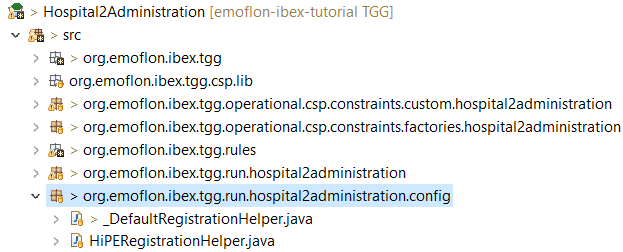
\includegraphics[scale=0.65 ]{pictures/registrationHelpers.png}
    \caption{\centering{Available registration helpers}}
    \label{setDefaultNumber}
\end{figure}

By default, a newly created project has the \textsf{\_DefaultRegistration} helper selected, but we recommend using the \textsf{HiPERegistrationHelper} for every application. \textbf{Exceptions} are the \textbf{BWD\_OPT} and the \textbf{FWD\_OPT} applications since both require the \textsf{DemoclesRegistrationHelper}.

The main difference between those two is the utilization of \textbf{different pattern matchers} which we have explained at the very beginning of our tutorial. 

\clearpage

\textbf{Saving and loading models:}

Let's look at further options within the applications:

\begin{figure}[h]
    \centering
    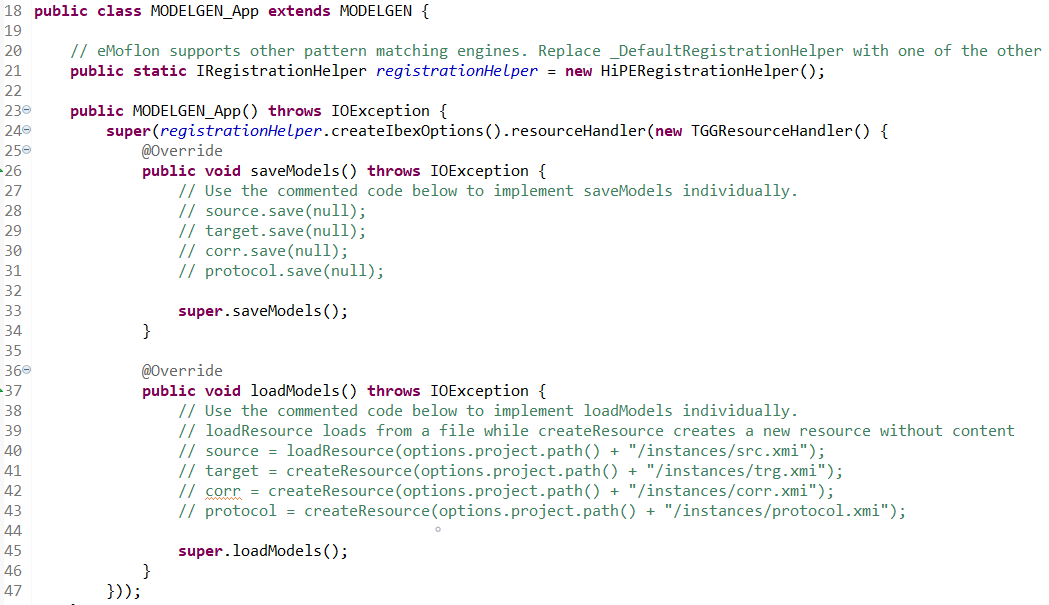
\includegraphics[scale=0.65 ]{pictures/application_MODELGEN.png}
    \caption{\centering{Example for loadModels() and saveModels() methods in the MODELGEN\_APP}}
    \label{setDefaultNumber}
\end{figure}

Depending on the operation you want to perform you can use the code which is commented out right now.\newline

\textbf{saveModels():}

This method is used to save specific components or the whole graph triplet. \textcolor{Purple}{super}.saveModels() saves all four files you can see in the instances folder. You can swap this out for one or multiple of the file specific save commands and insert a specific path for saving.\newline

\textbf{loadModels():}

This method is used to load specific components or a complete graph triplet.
For the individual load methods, we would load a model from the given path and create the corresponding resources.\newline

\textbf{Example:}

Let us walk through this exemplarily by modifying the \textsf{SYNC\_APP} to load the \textsf{hospital.xmi} we have created in the first part of this tutorial. First we want to modify the \textsf{loadModels} method to load the \textsf{hospital.xmi}.

You need to adjust the \textbf{path} to the source variable to access it. It should be saved in your workspace in the project folder of the \textsf{HospitalExample}. we will use a relative path to switch to the parent folder of our project directory then we navigate to the \textsf{hospital.xmi} which is stored in the project folder of our graph transformation project:\newline

39\hspace{0.5cm}\textcolor{Blue}{source} = loadResource(\textcolor{Blue}{options.project}.path() "\textcolor{Blue}{../HopsitalTransformationRules/hospital.xmi}");\newline

\clearpage

Since we want to synchronize our triple from the given source model, we have to create the other resources by using the \textsf{createResource} command which is commented out right now. Please remove the slash symbols for the following lines shown below:\newline

{\setstretch{1.2}

40\hspace{0.5cm}\textcolor{Blue}{target} = createResource(\textcolor{Blue}{options.project}.path() + "\textcolor{Blue}{/instances/trg.xmi}");

41\hspace{0.5cm}\textcolor{Blue}{corr} = createResource(\textcolor{Blue}{options.project}.path() + "\textcolor{Blue}{/instances/corr.xmi}");

42\hspace{0.5cm}\textcolor{Blue}{protocol} = createResource(\textcolor{Blue}{options.project}.path() + "\textcolor{Blue}{/instances/protocol.xmi}");\newline

}

After creating these resources, we still need to save them somewhere. Just uncomment the following lines in the \textsf{saveModels} method:\newline

{\setstretch{1.2}

40\hspace{0.5cm}\textcolor{Blue}{target}.save(\textcolor{Purple}{null});

41\hspace{0.5cm}\textcolor{Blue}{corr}.save(\textcolor{Purple}{null});

42\hspace{0.5cm}\textcolor{Blue}{protocol}.save(\textcolor{Purple}{null}); \newline

}

After you have saved your file and \textbf{ran} the \textbf{SYNC} application, look at the new instances. They should look different. If they are still the same, try deleting the files in the instances folder and rerun the App.

Now open up the \textsf{trg.xmi} and inspect it. The number of patients and staff members is much smaller now, but why?

In this case, we have loaded the \textsf{hospital.xmi} from our graph transformation project and in this model instance we have created the elements such as patients and staff members manually and the SYNC\_APP has generated our triple consisting of source, target, and correspondences according to the rules we defined in the TGG project. 

On the contrary, the MODELGEN\_APP created our consistent triple according to our TGG ruleset as well but \textbf{none of the values were bound} and hence the triple was created with random values as we defined it in the attribute conditions. Additionally, it would have done it \textbf{infinitely} if we had not defined the criteria to stop the execution of the application.\newline

You can find these criteria in the main method of the applications. For example, we set a stop criterion based on the runtime:\newline

\textcolor{Tan}{stop}.setTimeOutInMS(1000);\newline

For this example, we terminate our application after approximately \textsf{1000 ms}with the keyword \textcolor{Tan}{stop}. By using the auto-completion function you can see the other options you can set as \textbf{stop criteria}.

For example, if we want to execute a rule a certain number of times we can type:\newline

\textcolor{Tan}{stop}.setMaxRuleCount("HospitaltoAdministrationRule", 1); \newline

In this case, we limited the number of applications of the HospitalToAdministration to 1. You can find a list of possible stop criteria in the \textbf{appendix} below.

\clearpage

\subsection{ Debugging in TGGs}

A note on the debugging app you can find in the \textsf{.debug} package shown below:\newline

\begin{figure}[h]
    \centering
    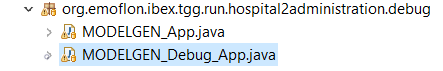
\includegraphics[scale=0.65 ]{pictures/debugPackage.png}
    \caption{\centering{\textsf{.debug} package}}
    \label{setDefaultNumber}
\end{figure}

There is no need for this when your set of triples is created without any errors. But when the rules or correspondences are not working in the way you want them to work you can run the generation in debug mode.

Once you run the \textsf{MODELGEN\_Debug\_App.java} a new window like the one in chart below pops up. On the top left, you can see the rules which have already been applied, the other rules are crossed out. On the right, you can see the respective visualization, and on the bottom left you can see the order in which the rules were applied. \newline

If you hit the \textbf{apply} button on the left now you will apply the next rule according to the way, we have defined it in the java files. This works like debugging in Java and leads you step by step through the application of our ruleset and updates of the visualization.

\begin{figure}[h]
    \centering
    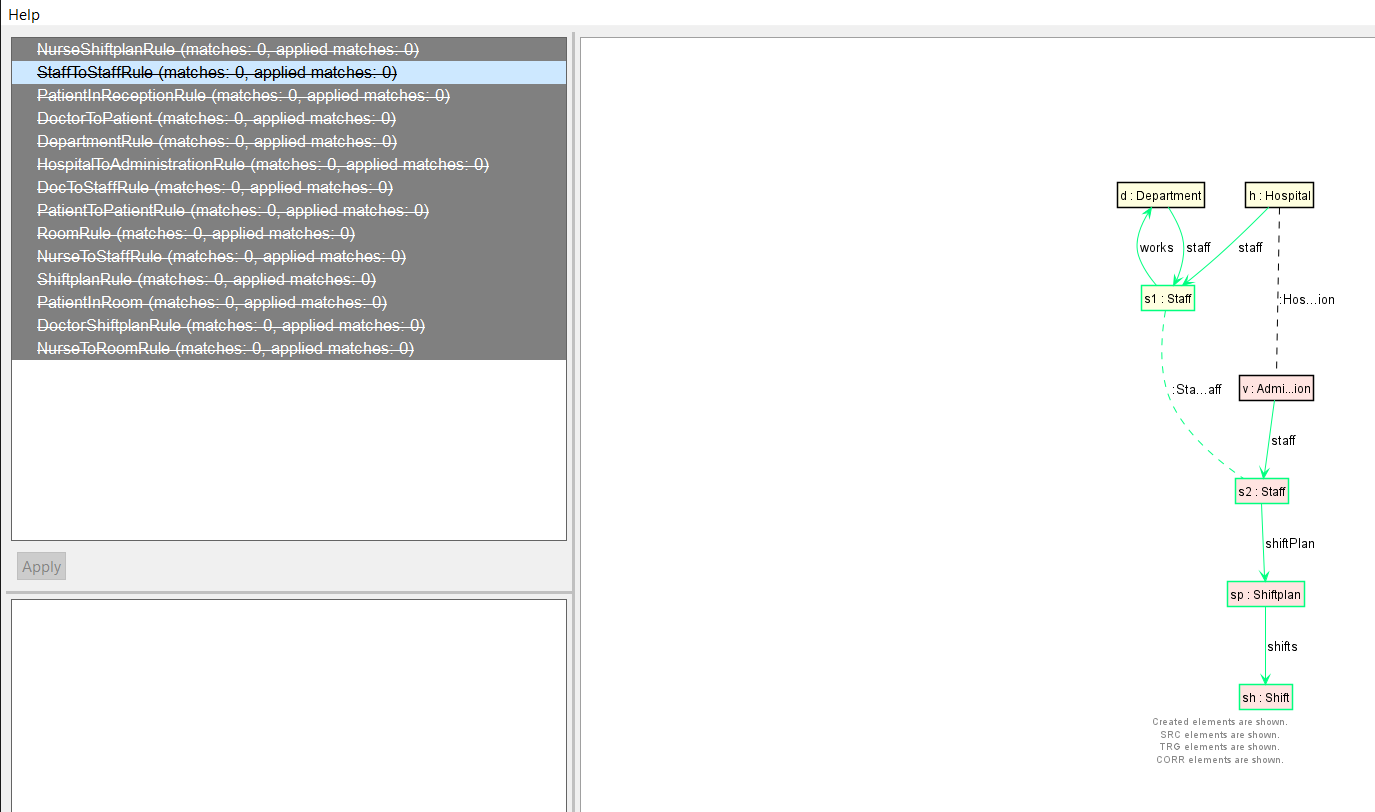
\includegraphics[scale=0.4 ]{pictures/debugWindow.png}
    \caption{\centering{Debugging window}}
    \label{setDefaultNumber}
\end{figure}


\clearpage
\section{Appendix for Triple Graph Grammars}

\subsection{Debugging the generated Pattern Invocation Networks (PIN):}

If you want to understand what is being provided as input to the underlying pattern matcher, or you are developing a new feature and need to “see” what is being passed as patterns, you can persist and visualize the so-called Pattern Invocation Network (PIN), which serves as input for the pattern matcher.

\begin{enumerate}

    \item In the app of your choice, e.g. MODELGEN\_App.java, locate the createIbexOptions method and append a debug(true) to the default statement in the method. This should return \_RegistrationHelper.createIbexOptions(). If you wish to switch on debug globally, you can change the value set in the \_RegistrationHelper
    
    \item Run the app with your change and refresh your TGG project. If you did things right, you should notice a newly created /debug folder in the project. If you open it,there should be two files: ibex-patterns.xmi and democles-patterns.xmi. These contain the same PIN but on different levels of abstraction: The former is independent of a specific pattern matcher, while the latter is precisely what Democles, the default pattern matcher, requires.
    
    \item In most cases, you will be interested in ibex-patterns.xmi. Opening this file will enable you to visualize the contained PIN in the PlantUML view. There is an overview visualization for the pattern set on the one hand and on the other is a visualization for individual context patterns.

\end{enumerate}

\clearpage

\subsection{Attribute conditions overview}

Here you can find a list of all default attribute conditions with a short description each. To look up all specific cases they cover take a look at the AttrCondDefLibrary.tgg in the org.emoflon.ibex.tgg.csp.lib package in your TGG project.\newline

{\setstretch{1.5}
\begin{center}
\begin{tabular}{ | m{6cm} | m{7cm} |  }
\hline
\textbf{Attribute condition} & \textbf{Description} \\
\hline
eq\_string(a: EString, b: EString)  & Ensures both given string variables are equal  \\
\hline
eq\_int(a: EInt, b: EInt)  & Ensures both given integer variables are equal  \\
\hline
eq\_float(a: EFloat, b: EFloat) & Ensures both given float variables are equal \\
\hline
eq\_double(a: EDouble, b: EDouble) & Ensures both given double variables are equal \\
\hline
eq\_long(a: ELong, b: ELong)  & Ensures both given long variables are equal \\
\hline
eq\_char(a: EChar, b: EChar) & Ensures both given char variables are equal \\
\hline
eq\_boolean(a: EBoolean, b: EBoolean) & Ensures both given boolean variables are equal \\
\hline
addPrefix(prefix:EString, word:EString, result:EString) & Adds a prefix to a given word variable and handing over the prefix plus the word as the result \\
\hline
addSuffix(suffix:EString, word:EString, result:EString)  & Adds a suffix to a given word variable and handing over the suffix plus the word as the result \\
\hline
concat(separator:EString, leftWord:EString, rightWord:EString, result:EString) & Combines a left word the separator and the right word in this order to a result \\
\hline
setDefaultString(variableString:EString, defaultString:EString) & Attribute condition which sets a variable string to the defaultString if it is free. \\
\hline
setDefaultNumber(variableNumber:EDouble, defaultNumber:EDouble) & Sets a variableNumber to the defaultNumber if it is free \\
\hline
stringToDouble(stringValue:EString, doubleValue:EDouble) & converts a stringValue into a double value \\
\hline
stringToInt(stringValue:EString, intValue:EInt) & Converts a stringValue into an int value \\
\hline
multiply(operand1:EDouble, operand2:EDouble, result:EDouble) & Multiplies both operands for the result \\
\hline
divide(numerator:EDouble, denominator:EDouble, result:EDouble)  & Divides the numerator by the denominator  and the result contains the solution of the operation \\
\hline
add(summand1:EDouble, summand2:EDouble, result:EDouble) & Adding both summands for the result \\
\hline
sub(minuend:EDouble, subtrahend:EDouble, result:EDouble)  & Subtracting the subtrahend from the minuend for the result \\
\hline
max(a:EDouble, b:EDouble, max:EDouble) & Selects the maximum value from the two given double variables \\
\hline
setRandomString(a:EString)  & Which sets a Variable to a random string. If it already has a value (B) then nothing is done and the condition is still satisfied \\
\hline

\end{tabular}
\end{center}
}

\clearpage

\subsection{Stop criterions overview}

{\setstretch{1.5}
\begin{center}
\begin{tabular}{ | m{6cm} | m{7cm} |  }
\hline
\textbf{Syntax} & \textbf{Description} \\
\hline
stop.setMaxElementCount(int maxElementCount) & Sets a stop criterion for the maximum number of elements allowed for the triple  \\
\hline
 stop.setMaxRuleCount(String ruleName, int maxNoOfApplications) & Sets a stop criterion for the defined number of applications for the named rule  \\
\hline
stop.setMaxSrcCount(int maxSrcCount) & Sets a stop criterion for the maximum number of elements allowed on the source side of a model instance \\
\hline
stop.setMaxTrgCount(int maxTrgCount) & Sets a stop criterion for the maximum number of elements allowed on the target side of a model instance \\
\hline
stop.setTimeOutInMs( long timeOutInMs) & Sets a stop criterion after the defined time in milliseconds has passed \\
\hline

\end{tabular}
\end{center}
}

\clearpage
\section{Troubleshooting}

\textbf{What are the best practices when specifying graph transformation rules?}

\begin{itemize}

    \item Use lowerCamelCase for patterns, rules, nodes, edges, and parameter names.
    
    \item Name the entities to methods and describe their purpose.
    
    \item Do not use node names like x, y, and z. Use descriptive names as you would do when writing a program. So, you do not lose track of their purpose. As the generated API uses the node names in methods this will lead to more traceable method names rather than getX().
    
    \item Try not to put everything into one file. You can reference patterns, rules, and conditions from other files within the same package.\newline
    
\end{itemize}

\textbf{I cannot specify a certain condition with the textual syntax. What can I do?}\newline

If your constraint cannot be expressed with eMoflon::IBeX application conditions, you can always apply additional arbitrary filtering conditions on the matches you get via the API using Java code.\newline\newline

\textbf{My meta-model code is not in a subpackage named the same as the metamodel. How can I fix the error in the generated API code?}\newline

By default, eMoflon::IBeX assumes that the code for your metamodel is in a package named like the package name in the Ecore file. If that is not the case for your metamodel, you can fix that with one of the following proposals:

\begin{itemize}

    \item Create a moflon.properties.xmi in the project’s root directory.
    
    \item Create a new “Import Mapping” within the “Moflon Properties Container”.
    
    \item Set the key to the URI as you reference your metamodel in the .gt files.
    
    \item Set the value to the name of the package containing generated code for your metamodel.\newline
    
\end{itemize}

\textbf{An EPackage seems to be in a different package. How can I fix such imports in the generated API code?}\newline

Similar to the question above, this problem can be resolved as follows:

\begin{itemize}

    \item Create a moflon.properties.xmi in the project’s root directory.
    
    \item Create a new “Import Mapping” within the “Moflon Properties Container”.
    
    \item Set the key to the error value of the EPackage import, which you would like to correct.
    
    \item Set the value to the corrected value of the import. Rebuild and check if the fix is as desired.\newline
    
\end{itemize}

\clearpage

\textbf{After the project build, errors the project has error markers. What do I have to do to resolve this issue?}

\begin{itemize}

    \item If the MANIFEST.MF is affected by the errors, try to build the project again and checks whether the error markers are removed. Try to build the project multiple times since some relations might not be built. Check for missing dependencies if rebuilding does not help. 
    
    \item If the plugin build creates the markers for missing packages before they are generated by the GT build, the error markers are removed as recently as the project is built again.
    
    \item If the errors are in generated code, check that you have added the metamodel project as a dependency of your project. Otherwise, Eclipse cannot find the metamodel classes on the build path of the GT project and reports errors.
    
    \item If none of the proposals above worked, you can try deleting the src-gen folder and building the whole project again. \newline

\end{itemize}

\textbf{I have switched to another branch of the repository for the tutorial, and I get error markers for my project?}

\begin{itemize}

    \item First, you should build your project. Try to build it multiple times if the errors persist.
    
    \item Secondly, you should look at the dependencies in the MANIFEST.MF, since the required bundles are not added automatically.
    
    \item If you still have errors in your project file you can try to delete the src-gen folder and rebuild the project.

\end{itemize}

\clearpage

%\bibliographystyle{plain}
%\bibliography{chapters/references}
	
\end{document}
